\documentclass[../vs-script-first-v01.tex]{subfiles}
\graphicspath{{\subfix{../}}}
\begin{document}


\section{Realisierung}
Bei der Implementierung von verteilten Systemen müssen mehrere Aspekte berücksichtigt werden, um sicherzustellen, dass das System effizient, zuverlässig und skalierbar ist. Eine umfassende Erörterung der Anforderungen in der Implementierung zu diskutieren ist aussichtslos, da eine nicht erfassbare Menge von Faktoren Einfluss haben. In den folgenden Punkten soll sich auf die grundsätzlichen Anforderungen an Prozesse und Kommunikation konzentriert werden. In den weiteren Kapiteln werden besondere Aspekte der Algorithmik, Koordination, Adressierung, wie auch Fehlertoleranz adressiert, bevor sich das Skript dem Testen und  dem Deployment zuwendet. 

\subsection{Prozesse und Threads}
Eine wesentliche Herausforderung ist die Organisation und die Strukturierung der Ablauffäden. Die kleinste, aus dem Modul Betriebssystemen, bekannte Struktur ist der Thread. Threads, implementiert auf einer node, bieten in verteilten Systemen mehrere Vorteile, die zu einer besseren Leistung, Ressourcennutzung und Reaktionsfähigkeit in einem verteilten System führen können:
\begin{itemize}
\item Parallelität: Threads ermöglichen die parallele Ausführung von Aufgaben innerhalb eines Prozesses, wodurch die Rechenressourcen (z.B. Mehrkernprozessoren) effizienter genutzt werden können. In verteilten Systemen kann dies dazu beitragen, dass mehrere Anfragen gleichzeitig auf einem Knoten verarbeitet werden, was zu einer schnelleren Reaktionszeit und einer besseren Leistung führt. Voraussetzung für die korrekte Einordnung des Mehrgewinns ist eine Unterscheidung in User- und Kernel-Threads.
\item Effiziente Ressourcennutzung: Da Threads innerhalb eines Prozesses ausgeführt werden, teilen sie sich den Speicher und andere Ressourcen. Dies ermöglicht eine effizientere Ressourcennutzung im Vergleich zur Verwendung von separaten Prozessen, die jeweils eigene Speicher- und Ressourcenbereiche haben. In verteilten Systemen kann dies dazu beitragen, den Gesamtressourcenverbrauch zu reduzieren. Hier liegt allerdings nicht der Fokus darauf die Threads über die gemeinsamen Ressourcen (z.B. Heap) zu koordinieren. Vielmehr verzichtet man vielmehr auf die Nutzung des gemeinsamen Speichers, um eine grundlegende Eigenschaft des verteilten Systems zu erhalten. Dies mag  im ersten Schritt merkwürdig klingen, erhält aber bei Einhaltung die Möglichkeit, die von den Threads umgesetzten Aufgaben auch auf Threads anderer Prozesse zu migrieren. Die Reduzierung liegt rein in der Reduzierung der Ressourcenverwwaltung, insbesondere auch dem Process Control Block.  

\item Reaktionsfähigkeit: Threads können unabhängig voneinander blockiert oder angehalten werden, während andere Threads im selben Prozess weiterlaufen. In verteilten Systemen kann dies dazu beitragen, die Reaktionsfähigkeit des Systems zu erhöhen, indem zeitaufwändige oder blockierende Aufgaben auf separate Threads ausgelagert werden, während andere Threads weiterhin Anfragen bedienen. Die Kontextwechsel sind im besten Fall leichter zu realisieren, als durch einen Prozess.

\item Granularität: Threads ermöglichen eine feinere Granularität bei der Parallelisierung von Aufgaben und können dazu beitragen, den Verwaltungsaufwand für die Verteilung von Aufgaben in verteilten Systemen zu reduzieren.
\end{itemize}
Trotz der Vorteile ist es wichtig, die Herausforderungen im Zusammenhang mit der Thread-Programmierung, wie z.B. Synchronisation, Deadlocks und Race Conditions, zu berücksichtigen und geeignete Techniken und Werkzeuge zur Bewältigung dieser Herausforderungen einzusetzen. Wichtig ist auch festzustellen, dass es für jede dieser Herausforderungen eine Lösung gibt, die aber verstanden und umgesetzt werden muss und jeweils mit negativen Eigenschaften belastet ist. Weiter kann auch auf besondere Eigenschaften der Threads verzichtet werden, um weiter die Defintion der verteilten Systemen zu erhalten um Mechanimsen, wie Skalierung, leichter zu etablieren.
\\\\
Die bereits angesprochene Abbildung der Threads im Betriebssystem ist weitere wesentliche Eigenschaft, die berücksichtigung finden muss. Es sollten hier zwei/drei Varianten unterschieden werden. Das \textbf{Many-to-One-Thread-Modell} ist ein Ansatz zur Verwaltung von Threads in einem Betriebssystem oder einer Anwendung, bei dem mehrere Benutzerthreads von einem einzigen Betriebssystem-Thread (\textbf{Kernel-Thread}) verwaltet werden. In diesem Modell werden die Benutzerthreads (\textbf{User-Threads})innerhalb der Anwendung geplant und ausgeführt, während der Kernel-Thread die Kommunikation und Interaktion mit dem Betriebssystem übernimmt. Vorteile und Nachteile des Many-to-One-Thread-Modells können wir beschreiben:
\begin{itemize}
\item Leichtgewicht: Da mehrere Benutzerthreads von einem einzigen Kernel-Thread verwaltet werden, sind die Ressourcenanforderungen für das System insgesamt geringer.
\item Portabilität: Da die Thread-Verwaltung auf Anwendungsebene erfolgt, ist das Many-to-One-Modell in der Regel unabhängig vom zugrunde liegenden Betriebssystem und daher portabeler zwischen verschiedenen Plattformen.
\item Skalierbarkeit: Da alle Benutzerthreads von einem einzigen Kernel-Thread verwaltet werden, kann das Modell nicht von Mehrkern- oder Mehrprozessorsystemen profitieren, da es keine echte Parallelität bietet.
\item Blockierung: Wenn ein Benutzerthread blockiert (z. B. aufgrund einer I/O-Operation), kann dies dazu führen, dass der gesamte Kernel-Thread blockiert wird und somit alle anderen Benutzerthreads zum Erliegen kommen.
\end{itemize}
Es existieren auch Alternativen zum Many-to-One-Thread-Modell, die wie folgt beschrieben werden können:
\begin{itemize}
\item \textbf{One-to-One-Thread-Modell}: In diesem Modell wird jedem Benutzerthread ein separater Kernel-Thread zugeordnet. Das One-to-One-Modell bietet bessere Skalierbarkeit und Parallelität, da mehrere Kernel-Threads gleichzeitig auf unterschiedlichen Kernen oder Prozessoren ausgeführt werden können. Allerdings kann es auch zu einer höheren Systembelastung führen, da mehr Ressourcen für die Verwaltung der Kernel-Threads benötigt werden.
\item \textbf{N:M-Thread-Modell} (auch bekannt als Many-to-Many-Thread-Modell): In diesem Modell gibt es eine variable Anzahl von Benutzerthreads und Kernel-Threads. Eine Gruppe von Benutzerthreads wird von einem oder mehreren Kernel-Threads verwaltet. Das N:M-Modell ermöglicht eine bessere Skalierbarkeit als das Many-to-One-Modell und kann bei der Ausnutzung von Mehrkern- oder Mehrprozessorsystemen effektiver sein. Es bietet auch eine gewisse Flexibilität bei der Zuordnung von Benutzerthreads zu Kernel-Threads, um den Anforderungen der Anwendung gerecht zu werden.
\end{itemize}
Jedes dieser Modelle hat seine Vor- und Nachteile. Die Wahl des am besten geeigneten Thread-Modells hängt von den Anforderungen der Anwendung, den verfügbaren Systemressourcen und der gewünschten Skalierbarkeit ab. Diese Aufzählung sollte auch primär der Auffrischung von Betriebssystemkenntnissen dienen. \\\\

\subsubsection{Threadpool}
Ein Threadpool ist ein Konzept in der Programmierung, bei dem eine bestimmte Anzahl von Threads im Voraus erstellt und verwaltet wird. Diese Threads werden zur parallelen Verarbeitung von Aufgaben in einer Warteschlange verwendet. Threadpools sind besonders nützlich, um die Systemressourcen effizient zu nutzen und die Leistung bei der Verarbeitung von vielen kleinen oder unabhängigen Aufgaben zu verbessern. Für parallele Aufgaben in einem homogenen und bekannten skalierenden System bietet dies ein breites Feld an Vorteilen. 
\begin{itemize}
\item Effiziente Ressourcennutzung: Da die Threads im Voraus erstellt und wiederverwendet werden, spart dies Zeit und Ressourcen, die sonst für das ständige Erstellen und Zerstören von Threads aufgewendet werden müssten.
\item Kontrolle über die Parallelität: Die Anzahl der Threads im Pool kann im Voraus festgelegt werden, um die Anzahl der gleichzeitig ausgeführten Aufgaben zu steuern und die Systemressourcen entsprechend zu nutzen.
\item Einfache Verwaltung: Ein Threadpool kümmert sich um die Verwaltung der Threads und die Zuweisung von Aufgaben, was die Komplexität bei der Verwaltung von Threads in der Anwendung reduziert.
\item Bessere Leistung: Threadpools können die Leistung verbessern, indem sie Wartezeiten reduzieren und die Reaktionsfähigkeit des Systems erhöhen.
\end{itemize}
Angenommen, es besteht eine Webanwendung, die eingehende Anfragen von Benutzern verarbeitet. Jede Anfrage kann unabhängig von den anderen bearbeitet werden und erfordert eine gewisse Rechenzeit. Anstatt für jede Anfrage einen neuen Thread zu erstellen, können Sie einen Threadpool verwenden. Hier ist ein einfaches Beispiel in Java, das einen Threadpool mit der ExecutorService-Klasse verwendet:\\\\

\begin{lstlisting}[caption={ExecutorService-Klasse},captionpos=b,label={lst:executor}]

import java.util.concurrent.ExecutorService;
import java.util.concurrent.Executors;

public class ThreadPoolExample {
    public static void main(String[] args) {
        int numThreads = 5;
        ExecutorService executor = Executors.newFixedThreadPool(numThreads);

        for (int i = 0; i < 10; i++) {
            Runnable task = new ExampleTask(i);
            executor.execute(task);
        }

        executor.shutdown();
    }
}

class ExampleTask implements Runnable {
    private int taskId;

    public ExampleTask(int taskId) {
        this.taskId = taskId;
    }

    @Override
    public void run() {
        System.out.println("Task " + taskId + " is running on thread: " + Thread.currentThread().getName());
    }
}
\end{lstlisting}
In diesem Beispiel erstellen wir einen Threadpool mit 5 Threads (numThreads). Der ExecutorService verwaltet den Threadpool und führt die ExampleTask-Instanzen aus. Da der Threadpool nur 5 Threads hat, werden maximal 5 Aufgaben (Tasks) gleichzeitig (im Zweifel nur Pseudoparallel) ausgeführt. Der ExecutorService sorgt dafür, dass alle Tasks in der Warteschlange abgearbeitet werden. Der Begriff des \textbf{Task} hat an dieser Stelle seinen Ursprung und findet in verteilten Systemen heute eine starke Nutzung.\\\\


Es gibt keine feste Regel für die maximale Auslastung eines Threadpools auf einer Node, da dies von der Anwendung und den Systemanforderungen abhängt. Ein allgemeiner Ansatz besteht darin, den Threadpool so zu konfigurieren, dass er die Anzahl der verfügbaren Prozessorkerne optimal nutzt. Als praktische Fausformel kann aber vielleicht mitgenommen werden, das ein Threadpool das gesamte System nicht mehr als 80 \% auslasten sollte.
Einige Empfehlungen für die Auslastung eines Threadpools auf einer Node sind:
\begin{itemize}
\item Berücksichtigen Sie die Art der Aufgaben, die der Threadpool ausführt. Bei rechenintensiven Aufgaben, die die CPU stark beanspruchen, ist es sinnvoll, die Anzahl der Threads auf die Anzahl der verfügbaren Prozessorkerne zu begrenzen. Bei Aufgaben, die auf I/O warten (z.B. Datei- oder Netzwerkzugriffe), kann es hilfreich sein, mehr Threads als Prozessorkerne zu verwenden, um die Wartezeiten besser auszugleichen.
\item Überwachen Sie die Systemauslastung und passen Sie die Größe des Threadpools bei Bedarf an. Wenn die CPU-Auslastung konstant hoch ist und die Anwendung langsamer wird, sollten Sie die Anzahl der Threads im Threadpool reduzieren. Wenn die CPU-Auslastung gering ist und viele Aufgaben auf I/O warten, können Sie die Anzahl der Threads im Threadpool erhöhen.
\end{itemize}
\paragraph{Task\\\\}

In verteilten Systemen bezieht sich der Begriff \enquote{Task} auf eine abstrakte Einheit von Arbeit oder eine Aufgabe, die von einem oder mehreren Komponenten innerhalb des Systems ausgeführt wird. Zur Wiederholung, ein verteiltes System besteht aus mehreren unabhängigen Rechnern oder Knoten, die zusammenarbeiten, um eine bestimmte Funktion oder einen bestimmten Prozess auszuführen. Wie festgestellt, ist das Worker-Thread-Pattern ein Entwurfsmuster, das häufig in verteilten Systemen verwendet wird, um die Verarbeitung von Tasks effizient zu handhaben. Ein gutes Design eines Tasks als Struktur zur Erfassung der Aufgabe sollte die folgenden Merkmale aufweisen:
\begin{itemize}
\item Modularität: Der Task sollte modular gestaltet sein, das heißt, er sollte in kleinere, unabhängige Einheiten zerlegt werden, die einzeln verarbeitet werden können. Dies ermöglicht eine einfachere Wiederverwendung von Code, erleichtert das Testen und ermöglicht es, das System bei Bedarf zu erweitern oder zu ändern.
\item Kapselung: Der Task sollte alle notwendigen Informationen und Ressourcen enthalten, um seine Arbeit auszuführen. Dies erleichtert das Verständnis der Task-Struktur, die Kommunikation zwischen den Systemkomponenten und die Fehlersuche im System.
\item Idempotenz: Wenn möglich, sollte der Task idempotent gestaltet sein, d.h. wenn er mehrmals mit den gleichen Eingaben ausgeführt wird, sollte er immer das gleiche Ergebnis liefern. Dies ist besonders wichtig in verteilten Systemen, in denen Fehler oder Netzwerkunterbrechungen dazu führen können, dass Tasks wiederholt oder neu gestartet werden müssen.
\item Zustandslosigkeit: Ein Task sollte zustandslos sein, das bedeutet, er sollte keine Informationen über frühere Ausführungen speichern. Zustandslose Tasks sind leichter zu verwalten und zu skalieren, da sie unabhängig voneinander auf verschiedenen Knoten ausgeführt werden können, ohne dass Informationen über den Zustand zwischen den Knoten synchronisiert werden müssen.
\item Fehlertoleranz: Der Task sollte so gestaltet sein, dass er bei Fehlern oder Ausfällen von Teilen des Systems weiterhin funktioniert. Dies kann durch Mechanismen wie Timeouts, Wiederholungsstrategien oder automatisches Failover erreicht werden.
\item Skalierbarkeit: Der Task sollte so gestaltet sein, dass er bei zunehmender Last oder Ressourcenanforderungen leicht skaliert werden kann. Das bedeutet, dass das System bei Bedarf einfach erweitert werden kann, indem zusätzliche Knoten oder Ressourcen hinzugefügt werden.
\item Kommunikation: Der Task sollte klar definierte Kommunikationsmechanismen und -protokolle verwenden, um Informationen zwischen den Systemkomponenten auszutauschen. Dies kann beispielsweise über Message Queues, Remote Procedure Calls (RPC) oder REST-APIs erfolgen.
\end{itemize}
Ein gut gestalteter Task bietet eine gute Grundlage für die Mechanismen der Skalierung. Hier sollte ausreichend Zeit in die Planung eingebracht werden.

\subsubsection{Multithreaded Clients}
In Multithreaded-Clients werden Threads häufig nicht nur zur Parallelisierung, sondern auch zur Organisation von Code und Aufgaben verwendet. Der Hauptgrund für diese Vorgehensweise ist, dass Multithreaded-Clients oft mit verschiedenen Arten von Aufgaben konfrontiert sind, die unabhängig voneinander und gleichzeitig ausgeführt werden müssen, um eine reibungslose Benutzererfahrung zu gewährleisten.
\\\\
Ein Webbrowser ist ein sehr gängiges Beispiel in diesem Kontext. Die Verwendung von Threads zur Organisation von Code und Aufgaben in solchen Fällen bietet mehrere Vorteile. Einige sollen beispielhaft diskutiert werden, die sich grundsätzlich über die Eigenschaften von Threads herleiten lassen:
\begin{itemize}
\item Reaktionsfähigkeit: Eine wichtige Anforderung für Client-Anwendungen ist, dass sie auf Benutzereingaben und Systemereignisse schnell reagieren können. Durch die Verwendung von Threads zur Organisation von Aufgaben können Benutzerinteraktionen und andere zeitkritische Prozesse unabhängig von zeitaufwändigen Hintergrundaufgaben (z. B. Dateioperationen, Netzwerkkommunikation) ausgeführt werden. Dies gewährleistet, dass die Anwendung auch während der Ausführung von langwierigen Aufgaben weiterhin reaktionsfähig bleibt.
\item Modularität und Wartbarkeit: Threads können verwendet werden, um Code und Aufgaben in logische, voneinander getrennte Einheiten zu organisieren. Dies verbessert die Lesbarkeit und Wartbarkeit des Codes, da jede Funktion oder Aufgabe innerhalb ihres eigenen Threads isoliert ist. Diese Modularität erleichtert auch das Debugging und die Fehlersuche in komplexen Anwendungen.
\item Bessere Ressourcennutzung: In einigen Fällen kann die Verwendung von Threads zur Organisation von Code und Aufgaben die Ressourcennutzung verbessern. Durch das Trennen von unabhängigen Aufgaben in separate Threads kann das System effizienter arbeiten, da es Ressourcen (z. B. Prozessorzeit) auf verschiedene Threads verteilt, anstatt sie einem einzigen, monolithischen Prozess zuzuweisen.
\item Vereinfachte Kommunikation: In Client-Anwendungen, die mit verschiedenen externen Diensten oder Datenquellen kommunizieren müssen, können Threads zur Organisation dieser Kommunikation verwendet werden. Indem jeder Kommunikationskanal in einem separaten Thread verwaltet wird, bleibt der Code für jeden Kanal sauber und leicht verständlich, während gleichzeitig das Risiko von Blockaden und Verzögerungen minimiert wird.
\end{itemize}
Ein einfaches Beispiel in Java, welches den Nutzen von Threads zur Organisation von Code und Aufgaben veranschaulicht, ist eine Anwendung, die eine Benutzerschnittstelle hat und gleichzeitig eine Datei herunterlädt. In diesem Beispiel bleiben die Benutzerschnittstelle und die Download-Aufgabe voneinander unabhängig, wodurch die Anwendung reaktionsfähig bleibt.\\\\
In diesem Beispiel des Listings~\ref{lst:down} wird ein separater Thread (downloadThread) erstellt, um den Download der Datei im Hintergrund durchzuführen. Während des Downloads kann der Hauptthread weiterhin Benutzereingaben über die Konsole akzeptieren und darauf reagieren, ohne von der Download-Aufgabe blockiert zu werden. Dies zeigt, wie Threads zur Organisation von Code und Aufgaben in einer Anwendung verwendet werden können, um eine bessere Reaktionsfähigkeit und Unabhängigkeit zwischen verschiedenen Aufgaben zu erreichen. Die Parallelisierung steht nicht immer im Vordergrund, obwohl die Erfassung nicht selten sinnvoll ist, dafür wird ein Maß eingeführt.

\paragraph{Thread-Level-Parallelism\\\\}
Thread-Level-Parallelism (TLP) ist ein Maß dafür, wie viele Threads in einer Anwendung gleichzeitig ausgeführt werden können. Eine Möglichkeit, TLP zu quantifizieren, besteht darin, den Speedup eines Programms zu berechnen, wenn es auf mehreren Threads parallel ausgeführt wird.\\\\

\noindent\begin{lstlisting}[caption={Threads zur Organisation},captionpos=b,label={lst:down}]
import java.io.BufferedInputStream;
import java.io.FileOutputStream;
import java.io.IOException;
import java.net.URL;
import java.util.Scanner;

public class DownloadExample {
    public static void main(String[] args) {
        Thread downloadThread = new Thread(() -> {
            System.out.println("Download-Thread gestartet");
            String fileUrl = "https://example.com/largefile.zip";
            String localFilename = "largefile.zip";

            try (BufferedInputStream in = new BufferedInputStream(new URL(fileUrl).openStream());
                 FileOutputStream fileOutputStream = new FileOutputStream(localFilename)) {
                byte[] dataBuffer = new byte[1024];
                int bytesRead;

                while ((bytesRead = in.read(dataBuffer, 0, 1024)) != -1) {
                    fileOutputStream.write(dataBuffer, 0, bytesRead);
                }
            } catch (IOException e) {
                e.printStackTrace();
            }

            System.out.println("Download abgeschlossen");
        });

        downloadThread.start();

        Scanner scanner = new Scanner(System.in);
        while (true) {
            System.out.println("Geben Sie 'exit' ein, um die Anwendung zu beenden");
            String input = scanner.nextLine();

            if (input.equalsIgnoreCase("exit")) {
                break;
            }

            System.out.println("Eingabe: " + input);
        }

        scanner.close();
    }
}
\end{lstlisting}

\begin{equation}
    Speedup = \frac{T_1}{T_p}
\end{equation}\\\\


Um TLP direkt zu berechnen, können wir den Speedup durch die Anzahl der Threads (p) teilen. Das Verhältnis gibt uns eine Idee davon, wie effektiv die parallele Ausführung auf mehreren Threads ist:

\begin{equation}
    TLP = \frac{Speedup}{p} = \frac{\frac{T_1}{T_p}}{p}
\end{equation}

Ein TLP von 1 würde bedeuten, dass das Programm perfekt parallelisiert ist, und jeder Thread gleichmäßig zur Reduzierung der Gesamtausführungszeit beiträgt. Ein TLP-Wert kleiner als 1 zeigt an, dass die parallele Ausführung weniger effektiv ist, da einige Threads möglicherweise auf Ressourcen warten oder es aufgrund von Synchronisationsproblemen zu Leistungsengpässen kommt.\\\\

Ein TLP von 1,5 bis 2 bedeutet, dass ein Webbrowser in der Lage ist, 1,5 bis 2 Threads gleichzeitig auszuführen, also einen Speedup unterstützt. Aber diese Zahl gibt auch an, dass ein Webbrowser nicht vollständig parallel ist. In diesem Beispiel können die Gründe dafür Vielfältig sein, Webbrowser müssen zahlreiche Aufgaben ausführen, wie das Laden und Darstellen von Webseiten, das Ausführen von JavaScript-Code, das Verarbeiten von Benutzereingaben und das Verwalten von Netzwerkanfragen. 
Webbrowser können somit eine gewisse Parallelität aufweisen, aber nicht extrem parallelisiert sein. Dies liegt daran, dass viele Aufgaben, die ein Browser ausführt, voneinander abhängig sind und eine gewisse Reihenfolge bei der Ausführung einhalten müssen. Zum Beispiel müssen HTML- und CSS-Ressourcen geladen und verarbeitet werden, bevor sie auf dem Bildschirm gerendert werden können, und JavaScript-Code kann die DOM-Struktur und das Erscheinungsbild einer Webseite verändern, was eine gewisse Synchronisation zwischen den Threads erfordert.
Ein TLP von 1,5 bis 2 bedeutet auch, dass Webbrowser die Ressourcen von modernen Multi-Core-Prozessoren nicht vollständig ausnutzen können. In vielen Fällen ist dies jedoch ausreichend, um eine gute Leistung und Benutzererfahrung zu gewährleisten.\\\\

Es ist wichtig zu beachten, dass der TLP-Wert von verschiedenen Faktoren abhängt, wie der Browserarchitektur, der verwendeten Webtechnologien und der Leistungsfähigkeit des zugrunde liegenden Systems. Daher kann der TLP-Wert für verschiedene Webbrowser und in verschiedenen Szenarien variieren.

\subsubsection{Single Threaded Process}
Ein Single-Threaded-Prozess ist ein Programm oder eine Anwendung, die nur einen einzigen Ausführungsstrang (Thread) verwendet, um Aufgaben nacheinander auszuführen. Dies steht im Gegensatz zu einem Multithreaded-Prozess, bei dem mehrere Threads parallel ausgeführt werden können, um gleichzeitig mehrere Aufgaben zu erledigen.

In einem Single-Threaded-Prozess werden die Aufgaben in einer sequenziellen Reihenfolge abgearbeitet, die durch den Programmfluss vorgegeben ist. Diese Art der Ausführung ist einfacher zu verstehen und zu programmieren, da keine Synchronisationsmechanismen oder Ressourcenschutzmaßnahmen erforderlich sind.\\\\

Ein Beispiel für die Umsetzung ist Node.js. Node.js ist eine serverseitige JavaScript-Laufzeitumgebung, die auf der V8-Engine von Google Chrome basiert. Eine der Hauptdesignphilosophien von Node.js ist die Verwendung eines Single-Threaded-Prozess, der asynchrone und ereignisgesteuerte I/O ermöglicht. Dies unterscheidet Node.js von vielen anderen serverseitigen Umgebungen, die auf Multithreading setzen, um mehrere gleichzeitige Anfragen zu verarbeiten. Der Single-Threaded-Prozess in Node.js bietet folgende Vorteile:
\begin{itemize}
\item Einfachheit: Da es nur einen Hauptthread gibt, entfallen die Probleme, die mit der Synchronisation von Threads, Deadlocks und Race Conditions verbunden sind. Dies vereinfacht den Programmieraufwand und reduziert die Wahrscheinlichkeit von schwer zu findenden Fehlern.
\item Skalierbarkeit: Node.js verwendet das ereignisgesteuerte Modell und asynchrone I/O-Aufrufe, um die Effizienz und Skalierbarkeit zu maximieren. Durch die Nichtblockierung von I/O-Aufrufen kann der Single-Threaded-Prozess eine große Anzahl gleichzeitiger Verbindungen effizient verwalten, ohne den Overhead, der durch das Erstellen und Verwalten mehrerer Threads entsteht.
\item Geringerer Ressourcenverbrauch: Da Node.js nur einen Thread verwendet, benötigt es weniger Systemressourcen wie Speicher und CPU im Vergleich zu serverseitigen Umgebungen, die mehrere Threads einsetzen. Dies kann insbesondere bei ressourcenbeschränkten Systemen von Vorteil sein. Es ist am Ende die einfachste Form einer Batch-Verarbeitung.
\end{itemize}
Ein einfaches Beispiel für einen Node.js-Server, der den Single-Threaded-Prozess verwendet, ist ein HTTP-Server, der Anfragen empfängt und verarbeitet:

\begin{lstlisting}[caption={Node.js Single Threaded},captionpos=b,label={lst:single}]
const http = require("http");
const server = http.createServer((req, res) => {
  console.log("Anfrage empfangen");

  // Simuliere eine zeitaufwaendige Operation
  setTimeout(() => {
    res.writeHead(200, { "Content-Type": "text/plain" });
    res.end("Hallo Welt!");
  }, 1000);
});
server.listen(3000, () => {
  console.log("Server laeuft auf Port 3000");
});
\end{lstlisting}
In diesem Beispiel erstellen wir einen einfachen HTTP-Server, der bei jeder Anfrage eine einsekündige Verzögerung simuliert. Da Node.js single-threaded ist, verwendet es asynchrone I/O-Aufrufe (in diesem Fall setTimeout), um die Verzögerung zu implementieren, ohne den Hauptthread zu blockieren. Während der Verzögerung kann der Hauptthread weiterhin neue Anfragen empfangen und verarbeiten.
\\\\
Acuh wenn der Single-Threaded-Prozess von Node.js in vielen Situationen Vorteile bietet, hat er auch seine Grenzen. Zum Beispiel kann der Single-Threaded-Prozess die Rechenleistung von Mehrkernprozessoren ohne weiteres nicht voll ausnutzen, und rechenintensive Aufgaben können die Leistungsfähigkeit des Servers beeinträchtigen. In solchen Fällen kann es sinnvoll sein, Techniken wie Clustering, Worker-Threads oder alternative Architekturen zu verwenden, um die Leistung und Skalierbarkeit der Anwendung zu verbessern.
\paragraph{Blocking vs non-blocking\\\\}
Parallelisierung und Blockierung (Blocking) sowie Nicht-Parallelisierung und Nicht-Blockierung (Non-blocking) sind zwei verschiedene Ansätze zur Programmierung und Systemgestaltung, die jeweils ihre eigenen Vor- und Nachteile haben, wobei die Non-Blocking Variante in Single-Threaded-Prozesse eine besondere Rolle haben, da sie viele Vorteile hat. 
\begin{itemize}
\item Höhere Skalierbarkeit: Non-Blocking I/O ermöglicht es, mehr gleichzeitige Verbindungen oder Anfragen mit weniger Ressourcen (z.B. Threads oder Prozesse) zu verwalten, was zu einer besseren Skalierbarkeit führt.
\item Bessere Leistung: Da Non-Blocking I/O Threads oder Prozesse nicht blockiert, können diese Ressourcen für andere Aufgaben verwendet werden, wodurch die Gesamtleistung des Systems verbessert wird.
\item Reduzierte Latenz: Non-Blocking I/O ermöglicht es, dass mehrere I/O-Operationen gleichzeitig ausgeführt werden, wodurch die Gesamtlatenz für das Abschließen einer Gruppe von Operationen reduziert wird.
\end{itemize}
Non-Blocking I/O-Techniken werden häufig in serverseitigen Anwendungen wie Webservern, Datenbanken und anderen Netzwerkdiensten eingesetzt, um eine höhere Skalierbarkeit und bessere Leistung zu erzielen. Es gibt verschiedene Ansätze, um Non-Blocking I/O im Netzwerkbereich zu implementieren:
\begin{itemize}
\item Asynchrone I/O (AIO): Asynchrone I/O-Operationen ermöglichen es, dass ein Thread oder Prozess eine I/O-Operation startet und sofort zur nächsten Anweisung übergeht, ohne auf das Ergebnis der Operation zu warten. Das Betriebssystem benachrichtigt den Thread oder Prozess, wenn die I/O-Operation abgeschlossen ist, normalerweise über Callback-Funktionen oder Ereignisse.
\item I/O-Multiplexing (auch bekannt als Event-Driven I/O): Bei dieser Technik wird ein zentrales Ereignishandling-System verwendet, um auf mehrere I/O-Operationen gleichzeitig zu warten und das Programm über abgeschlossene Operationen zu informieren. Beispiele für I/O-Multiplexing-APIs sind select, poll und epoll in Unix/Linux-Systemen.
\item Non-Blocking Sockets: Dieser Ansatz verwendet spezielle Socket-Optionen, um Netzwerkoperationen wie send und recv in einem Nicht-Blockiermodus auszuführen. Auch wenn die Operation nicht sofort abgeschlossen werden kann, gibt die Funktion sofort zurück und zeigt an, dass die Operation später erneut versucht werden sollte.
\end{itemize}
Trotz der Vorteile sollte verstanden sein, dass die Programmierung von Non-Blocking I/O im Netzwerkbereich komplexer sein wird, als die Verwendung von blockierenden I/O-Operationen, da Entwickler zusätzliche Mechanismen für das Ereignishandling und die Synchronisation implementieren müssen.
\\\\
Ein Beispiel für Non-Blocking I/O ist in Java die Verwendung von java.nio-Paketen, welche asynchrone und Non-Blocking I/O-Operationen unterstützen. In diesem Beispiel erstellen wir einen einfachen Echo-Server, der Non-Blocking I/O mit java.nio.channels verwendet:

\begin{lstlisting}[caption={Non-Blocking},captionpos=b,label={lst:nonb}]
import java.io.IOException;
import java.net.InetSocketAddress;
import java.nio.ByteBuffer;
import java.nio.channels.SelectionKey;
import java.nio.channels.Selector;
import java.nio.channels.ServerSocketChannel;
import java.nio.channels.SocketChannel;
import java.util.Iterator;
import java.util.Set;

public class NonBlockingEchoServer {
    public static void main(String[] args) throws IOException {
        // Create a new selector
        Selector selector = Selector.open();

        // Create a new server socket channel and bind it to a port
        ServerSocketChannel serverSocketChannel = ServerSocketChannel.open();
        serverSocketChannel.bind(new InetSocketAddress(8000));

        // Configure the server socket channel to be non-blocking
        serverSocketChannel.configureBlocking(false);

        // Register the server socket channel with the selector for accepting new connections
        serverSocketChannel.register(selector, SelectionKey.OP_ACCEPT);

        while (true) {
            // Wait for events
            int readyChannels = selector.select();

            if (readyChannels == 0) {
                continue;
            }

            Set<SelectionKey> selectedKeys = selector.selectedKeys();
            Iterator<SelectionKey> keyIterator = selectedKeys.iterator();

            while (keyIterator.hasNext()) {
                SelectionKey key = keyIterator.next();

                if (key.isAcceptable()) {
                    // Accept the new connection
                    ServerSocketChannel serverChannel = (ServerSocketChannel) key.channel();
                    SocketChannel socketChannel = serverChannel.accept();

                    // Configure the new socket channel to be non-blocking
                    socketChannel.configureBlocking(false);

                    // Register the new socket channel with the selector for reading data
                    socketChannel.register(selector, SelectionKey.OP_READ);
                } else if (key.isReadable()) {
                    // Read the data from the socket channel
                    SocketChannel socketChannel = (SocketChannel) key.channel();
                    ByteBuffer buffer = ByteBuffer.allocate(256);
                    int bytesRead = socketChannel.read(buffer);

                    if (bytesRead == -1) {
                        // Close the socket channel if the client has disconnected
                        socketChannel.close();
                    } else {
                        // Echo the data back to the client
                        buffer.flip();
                        socketChannel.write(buffer);
                    }
                }

                keyIterator.remove();
            }
        }
    }
}
\end{lstlisting}
Das Listing~\ref{lst:nonb} seigt einen Selector, um gleichzeitig mehrere Verbindungen zu verwalten. Der Echo-Server liest Daten von verbundenen Clients und sendet die empfangenen Daten sofort an den jeweiligen Client zurück.

\subsubsection{Serveranwendungen}
Bei der Entwicklung von Serveranwendungen kann die Architektur entweder auf einem iterativen (sequentiellen) oder einem nebenläufigen (Concurrent) Ansatz basieren. Beide Ansätze haben ihre eigenen Vor- und Nachteile, abhängig von den Anforderungen der Anwendung und den zugrunde liegenden Systemressourcen. 

Ein \textbf{iterativer Server} verarbeitet Anfragen sequenziell, d.h. er verarbeitet eine Anfrage vollständig, bevor er zur nächsten übergeht.  Durch die Verwendung des iterativen Servers ergeben sich Vorteile wie Nachteile:
\begin{itemize}
\item Einfache Implementierung: Iterative Server sind einfacher zu entwickeln und zu warten, da sie keine komplexen nebenläufigen Programmierkonzepte erfordern. Es müssen keine Nebenläufigkeitsprobleme, wie Synchronisation, Deadlocks oder Race Conditions, berücksichtigt werden.
\item Geringerer Ressourcenverbrauch: Da keine zusätzlichen Threads oder Prozesse erstellt werden, verbraucht ein iterativer Server in der Regel weniger Ressourcen wie Speicher und CPU.
\item Skalierbarkeit: Da ein iterativer Server Anfragen sequenziell verarbeitet, kann er bei einer großen Anzahl gleichzeitiger Anfragen schnell überlastet werden und zu einer schlechten Leistung führen. Das Warteschlangen-Modell kann auch hier Antworten bieten.
\item Reaktionsfähigkeit: Wenn eine Anfrage zeitaufwändige oder blockierende Operationen beinhaltet, werden nachfolgende Anfragen verzögert, was zu einer schlechteren Benutzererfahrung führen kann.
\end{itemize}
Ein \textbf{nebenläufiger Server} verwendet Threads oder Prozesse, um mehrere Anfragen gleichzeitig zu verarbeiten. Dadurch kann der Server eine größere Anzahl von Anfragen effizienter verarbeiten und eine bessere Reaktionsfähigkeit bieten. Auch Concurrent Server haben Vorteile wie Nachteile:

\begin{itemize}
\item Skalierbarkeit: Durch die Verwendung von Threads oder Prozessen zur gleichzeitigen Verarbeitung von Anfragen kann ein nebenläufiger Server eine größere Anzahl gleichzeitiger Verbindungen bewältigen und eine bessere Leistung bieten.
\item Reaktionsfähigkeit: Da jeder Thread oder Prozess unabhängig von den anderen arbeitet, können nebenläufige Server auch bei zeitaufwändigen oder blockierenden Operationen eine bessere Reaktionsfähigkeit bieten.
\item Komplexität: Die Implementierung eines nebenläufigen Servers erfordert ein besseres Verständnis von nebenläufigen Programmierkonzepten wie Synchronisation, Deadlocks und Race Conditions. Dies kann zu einer komplexeren und fehleranfälligeren Implementierung führen.
\end{itemize}
Die Wahl zwischen einem iterativen und einem nebenläufigen Server hängt von den Anforderungen der Anwendung und den Ressourcen des Systems ab. Für Anwendungen mit geringem Verkehrsaufkommen und einfachen Anforderungen kann ein iterativer Server ausreichend sein. Hier sind zwei einfache Beispiele in Listing~\ref{lst:iterativ} und Listing~\ref{lst:concurrent} für einen iterativen und einen nebenläufigen Server in Java unter Verwendung des java.net-Pakets:
\begin{lstlisting}[caption={Iterativer Server},captionpos=b,label={lst:iterativ}]
import java.io.IOException;
import java.io.InputStream;
import java.io.OutputStream;
import java.net.ServerSocket;
import java.net.Socket;

public class IterativeServer {
    public static void main(String[] args) throws IOException {
        int port = 1234;
        ServerSocket serverSocket = new ServerSocket(port);

        while (true) {
            Socket clientSocket = serverSocket.accept();
            handleClient(clientSocket);
            clientSocket.close();
        }
    }

    public static void handleClient(Socket clientSocket) throws IOException {
        InputStream input = clientSocket.getInputStream();
        byte[] buffer = new byte[1024];
        int bytesRead = input.read(buffer);
        System.out.println("Received: " + new String(buffer, 0, bytesRead));

        OutputStream output = clientSocket.getOutputStream();
        output.write("Hello, Client!".getBytes());
    }
}
\end{lstlisting}
In dem Listing des iterativen Serves erkennen wir einen einfachen Echo-Server, der die vom Client gesendeten Nachrichten empfängt und eine Antwort zurücksendet. Der iterative Server verarbeitet die Anfragen nacheinander, während der nebenläufige Server in Listing~\ref{lst:concurrent} für jede Anfrage einen neuen Thread erstellt, um sie gleichzeitig zu verarbeiten, dies ist im folgenden Beispiel erkennbar.

\begin{lstlisting}[caption={Concurrent Server},captionpos=b,label={lst:concurrent}]
import java.io.IOException;
import java.io.InputStream;
import java.io.OutputStream;
import java.net.ServerSocket;
import java.net.Socket;

public class ConcurrentServer {
    public static void main(String[] args) throws IOException {
        int port = 1234;
        ServerSocket serverSocket = new ServerSocket(port);

        while (true) {
            Socket clientSocket = serverSocket.accept();
            new Thread(() -> {
                try {
                    handleClient(clientSocket);
                } catch (IOException e) {
                    e.printStackTrace();
                } finally {
                    try {
                        clientSocket.close();
                    } catch (IOException ex) {
                        ex.printStackTrace();
                    }
                }
            }).start();
        }
    }

    public static void handleClient(Socket clientSocket) throws IOException {
        InputStream input = clientSocket.getInputStream();
        byte[] buffer = new byte[1024];
        int bytesRead = input.read(buffer);
        System.out.println("Received: " + new String(buffer, 0, bytesRead));

        OutputStream output = clientSocket.getOutputStream();
        output.write("Hello, Client!".getBytes());
    }
}
\end{lstlisting}

\subsubsection{Prozesse}

In verteilten Systemen spielen Prozesse eine entscheidende Rolle für die Organisation und Durchführung von Aufgaben. Im Kontext von verteilten Systemen bezieht sich der Begriff \enquote{Prozess} häufig auf einen laufenden Task oder eine Anwendung, die auf einem der Knoten im System ausgeführt wird oder, in einer groberen Granularität, einen Dienst (Service). In verteilten Systemen können mehrere Prozesse gleichzeitig auf verschiedenen Knoten (nodes) ausgeführt werden, um die Leistung und Effizienz des Systems zu steigern. Dies ermöglicht eine schnellere Verarbeitung von Aufgaben und eine bessere Auslastung der Ressourcen. 
Die Möglichkeit, Prozesse auf verschiedenen Knoten auszuführen, ermöglicht es verteilten Systemen, die Last auf die verfügbaren Ressourcen zu verteilen und bei Bedarf zu skalieren. Wenn die Systemlast zunimmt, können zusätzliche Knoten hinzugefügt werden, um die Leistung zu erhöhen und die Ausführung der Prozesse zu beschleunigen. Prozesse in verteilten Systemen können so konzipiert sein, dass sie bei Ausfällen oder Fehlern in anderen Teilen des Systems weiterhin funktionieren (Fehlertolerant). Dies kann durch redundante Prozesse, Replikation oder automatisches Failover erreicht werden. Diese Techniken werden im Folgenden noch besprochen. Ein weiterer Vorteil ist, Prozesse können unabhängig voneinander entwickelt, getestet und gewartet werden. Dies erleichtert die Implementierung von Änderungen und die Isolierung von Fehlern. \\\\

Eine wesentliche Herausforderung ist, dass in verteilten Systemen Prozesse miteinander kommunizieren müssen, um Informationen auszutauschen. Die Kommunikation zwischen Prozessen kann über verschiedene Mechanismen erfolgen, wie z. B. Message Passing, Remote Procedure Calls (RPC) oder REST-APIs. Grundlage ist aber meist die Interprocess-Kommunikation (IPC).
Neben der Kommunikation ist aber auch die Portierung der Prozesse auf verschiedene Orte eine besondere Herausforderung, auch um die Verteilungstransparenz und die Skalierung über die Problemgröße zu erreichen. \\\\
Selbst beterogene Systeme bestehen aus unterschiedlichen Hardware- und Softwarekomponenten, wie z. B. verschiedene Prozessorarchitekturen, Betriebssysteme oder Netzwerkprotokolle. Diese Unterschiede können zu Problemen bei der Portierung führen, darunter aus anderen Modulen bekannte Probleme:
\begin{itemize}
\item Unterschiedliche Prozessorarchitekturen: Verschiedene Systeme können unterschiedliche Prozessortypen verwenden (z. B. x86, ARM, MIPS), die jeweils eigene Befehlssätze und Spezifikationen haben. Bei der Portierung von Prozessen müssen diese Unterschiede berücksichtigt werden, und der Code muss möglicherweise angepasst oder neu kompiliert werden, um auf der Zielplattform korrekt zu funktionieren.
\item Betriebssystemabhängigkeiten: Prozesse können Funktionen oder APIs verwenden, die spezifisch für ein bestimmtes Betriebssystem sind. Bei der Portierung auf ein anderes Betriebssystem müssen diese Abhängigkeiten identifiziert und angepasst werden, um Inkompatibilitäten zu vermeiden.
\item Byte-Reihenfolge (Endianess): Unterschiedliche Systeme können unterschiedliche Byte-Reihenfolgen verwenden (Big-Endian oder Little-Endian). Dies kann zu Problemen bei der Interpretation von Daten führen, die zwischen Systemen ausgetauscht werden. Bei der Portierung von Prozessen muss die Byte-Reihenfolge berücksichtigt und möglicherweise konvertiert werden, um eine korrekte Kommunikation und Datenverarbeitung zu gewährleisten.
\item Speicherverwaltung: Verschiedene Systeme können unterschiedliche Speicherverwaltungsmechanismen verwenden, z. B. hinsichtlich der Speicherzuweisung, Freigabe oder Adressierung. Bei der Portierung von Prozessen müssen diese Unterschiede berücksichtigt werden, und der Code muss möglicherweise angepasst werden, um auf der Zielplattform korrekt zu funktionieren.
\item Kommunikationsprotokolle: In heterogenen Systemen können unterschiedliche Kommunikationsprotokolle oder Netzwerkstandards zum Einsatz kommen. Bei der Portierung von Prozessen müssen diese Unterschiede berücksichtigt werden, und es müssen möglicherweise Anpassungen an der Kommunikationsschnittstelle vorgenommen werden, um eine korrekte Interaktion zwischen den Komponenten zu ermöglichen.
\item Leistungsunterschiede: Unterschiedliche Hardwarekomponenten in heterogenen Systemen können zu unterschiedlichen Leistungsniveaus führen. Bei der Portierung von Prozessen sollten diese Unterschiede berücksichtigt werden, um sicherzustellen, dass die Anwendung auf der Zielplattform effizient und performant arbeitet.
\item Softwarebibliotheken und Frameworks: Prozesse können von externen Softwarebibliotheken oder Frameworks abhängig sein, die möglicherweise nicht auf der Zielplattform verfügbar sind oder unterschiedliche Versionen aufweisen. Bei der Portierung müssen solche Abhängigkeiten identifiziert und angepasst werden, um Inkompatibilitäten zu vermeiden.
\end{itemize}
Um die Portierung von Prozessen auf heterogenen Systemen erfolgreich durchzuführen, sind einige Strategien und Techniken hilfreich:
\begin{itemize}
\item Abstraktion: Verwenden Sie Abstraktionsschichten, um plattformspezifische Details zu kapseln und einen gemeinsamen Satz von Schnittstellen für die Anwendung bereitzustellen. Dadurch wird die Portierung erleichtert, da nur die plattformspezifischen Implementierungsdetails angepasst werden müssen.
\item Plattformunabhängige Programmiersprachen und Laufzeitumgebungen: Verwenden Sie plattformunabhängige Programmiersprachen (z. B. Java, Python) oder Laufzeitumgebungen (z. B. .NET Core), die auf verschiedenen Plattformen ausgeführt werden können. Diese Technologien ermöglichen es, den Code einmal zu schreiben und auf mehreren Plattformen auszuführen, was die Portierungsaufwände reduziert.
\item Standardbibliotheken und Protokolle: Nutzen Sie standardisierte Bibliotheken, Frameworks und Kommunikationsprotokolle, die auf verschiedenen Plattformen verfügbar und kompatibel sind. Dies erleichtert die Portierung, da die Abhängigkeiten und Schnittstellen zwischen den Systemkomponenten konsistent bleiben.
\item Cross-Kompilierung: Verwenden Sie Cross-Kompiler, um den Code für verschiedene Zielplattformen zu kompilieren. Dies ermöglicht eine bessere Kontrolle über die Erstellung von Binärdateien, die auf verschiedenen Prozessorarchitekturen ausgeführt werden können.
\item Automatisiertes Testen: Stellen Sie sicher, dass Sie umfangreiche Testsuiten haben, die alle wichtigen Funktionen Ihrer Anwendung abdecken. Automatisierte Tests sind besonders wichtig bei der Portierung von Prozessen, da sie dabei helfen, Fehler und Inkompatibilitäten schnell zu erkennen und zu beheben.
\item Dokumentation und Wissenstransfer: Eine gute Dokumentation der Anwendung, der verwendeten Technologien und der plattformspezifischen Details ist entscheidend für den Erfolg der Portierung. Der Wissenstransfer zwischen den Entwicklern, die an der Portierung beteiligt sind, hilft dabei, mögliche Probleme zu identifizieren und effizient zu lösen.
\end{itemize}
Indem diese Strategien und Techniken angewendet werden, können die Herausforderungen bei der Portierung von Prozessen auf heterogenen Systemen besser bewältigt werden, und die Wahrscheinlichkeit eines erfolgreichen Portierungsprojekts wird erhöht. Aber auch wenn selbst die Portierung und die Etablierung auf singulärer Hardware ausreicht, sind weitere Herausforderungen zu berücksichtigen. Beispielhaft, wenn mehrere Prozesse auf derselben Hardware ausgeführt werden, können Isolations- und Sicherheitsprobleme auftreten. Einige der häufigsten Probleme sind:
\begin{itemize}
\item Speicherzugriffsverletzungen: Wenn Prozesse auf demselben System ausgeführt werden, besteht das Risiko, dass sie auf den Speicherbereich eines anderen Prozesses zugreifen und somit Daten beschädigen oder korrumpieren. Moderne Betriebssysteme implementieren Speicherschutzmechanismen, um den Speicherbereich jedes Prozesses voneinander zu isolieren. Dennoch kann es aufgrund von Fehlern oder Schwachstellen in der Software zu unerwünschten Speicherzugriffen kommen.
\item Ressourcenkonflikte: Mehrere Prozesse, die auf derselben Hardware laufen, müssen sich die verfügbaren Ressourcen teilen, wie z. B. CPU, Speicher, I/O-Geräte und Netzwerkbandbreite. Ressourcenkonflikte können zu Leistungseinbußen, unvorhersehbarem Verhalten oder Systeminstabilität führen.
\item Nebenkanalangriffe: Bei Nebenkanalangriffen nutzt ein Angreifer Informationen, die durch die Ausführung von Prozessen auf derselben Hardware unbeabsichtigt preisgegeben werden, um vertrauliche Daten abzuleiten. Beispiele sind Cache-Timing-Angriffe oder die Spectre- und Meltdown-Schwachstellen, die aufgrund von Hardware-Designfehlern in modernen Prozessoren entstanden sind.
\item Privilegienerweiterung: Ein Prozess, der in der Lage ist, höhere Berechtigungen oder Systemressourcen zu erlangen, als ihm ursprünglich zugewiesen wurden, kann die Sicherheit und Isolation anderer Prozesse gefährden. Ein Angreifer kann solche Schwachstellen ausnutzen, um auf vertrauliche Daten zuzugreifen oder die Kontrolle über das System zu erlangen.
\item Prozess-Interaktionen: Wenn Prozesse auf demselben System interagieren, etwa über Interprozesskommunikation (IPC) oder gemeinsam genutzte Ressourcen, kann dies Sicherheitsrisiken bergen. Ein Angreifer kann versuchen, solche Interaktionen zu manipulieren, um Daten abzufangen oder Prozesse zu beeinflussen.
\end{itemize}
Um die Isolation und Sicherheit von Prozessen auf derselben Hardware zu gewährleisten, können verschiedene Maßnahmen ergriffen werden:
\begin{itemize}
\item Zugriffskontrolle: Implementierung strenger Zugriffskontrollmechanismen, um sicherzustellen, dass Prozesse nur auf die Ressourcen zugreifen können, die sie benötigen.
\item Sandboxen: Prozesse werden in isolierten Umgebungen ausgeführt, z. B. in Containern oder virtuellen Maschinen, um die Isolation zwischen Prozessen zu verbessern und die Angriffsfläche zu reduzieren.
\item Überwachung und Auditing: Überwachung der Aktivitäten von Prozessen, um verdächtiges Verhalten oder Sicherheitsverletzungen frühzeitig zu erkennen.
\item Sicherheitspatches: Betriebssystem und die Anwendungssoftware auf dem neuesten Stand halten, indem regelmäßig Sicherheitspatches und Updates installiert werden. Dies hilft, bekannte Schwachstellen zu beheben, die von Angreifern ausgenutzt werden könnten.
\item Prinzip der geringsten Privilegien: Prozesse nur die minimal erforderlichen Berechtigungen zuweisen. Dies reduziert das Risiko von Privilegienerweiterungsangriffen und minimiert die potenziellen Schäden, die ein kompromittierter Prozess verursachen kann.
\item Kryptografie: Nutzung von kryptografische Verfahren, um vertrauliche Daten in Speicher und während der Übertragung zu schützen. Dies verhindert, dass Angreifer auf sensible Informationen zugreifen können, selbst wenn sie Zugang zu einem kompromittierten Prozess erhalten.
\item Prozess-Isolation auf Hardware-Ebene: Einige Prozessoren und Plattformen bieten Hardware-unterstützte Funktionen zur Isolation von Prozessen, wie z. B. Intel's Software Guard Extensions (SGX) oder ARM's TrustZone. Durch die Nutzung dieser Funktionen kann die Isolation und Sicherheit von Prozessen auf derselben Hardware verbessert werden.
\item Sicherheitsbewusstes Design und Entwicklung: Sicherheit von Anfang an in den Entwicklungsprozess integrieren. Verwendung sicherer Programmierpraktiken und Durchführung regelmäßiger Sicherheitsanalysen und -prüfungen durch, um Schwachstellen frühzeitig zu identifizieren und zu beheben.
\end{itemize}
Indem diese Maßnahmen umgesetzt werden, können die Isolation und Sicherheit verbessert und potenzielle Sicherheitsrisiken minimiert werden. Es ist wichtig, einen mehrschichtigen Sicherheitsansatz zu verfolgen und auf allen Ebenen des Systems für eine robuste Verteidigung zu sorgen.

\subsubsection{Prozessverwaltung}
Distributed Operating Systems (DOS) und Network Operating Systems (NOS) sind zwei Ansätze zur Verwaltung von Prozessen in verteilten Systemen. Hier ist zunächst ein Überblick über die Hauptmerkmale von DOS, gefolgt von einem Beispiel aus der Praxis:
\begin{itemize}
\item Transparenz: DOS zielt darauf ab, die Verteilung der Ressourcen und Prozesse im System weitgehend zu verbergen. Das bedeutet, dass die Benutzer und Anwendungen das verteilte System als einen einzigen, kohärenten Computer wahrnehmen, obwohl es aus mehreren, vernetzten Knoten besteht.
\item Globale Ressourcenverwaltung: In einem DOS werden Ressourcen wie Speicher, Prozessorleistung und I/O-Geräte zentral verwaltet und den Prozessen im System zugewiesen. Dies ermöglicht eine effiziente Nutzung der verfügbaren Ressourcen und fördert Lastverteilung und Fehlertoleranz.
\item Prozessmigration: DOS ermöglicht die Migration von Prozessen zwischen verschiedenen Knoten im verteilten System. Dies kann dazu beitragen, die Ausführungsgeschwindigkeit zu verbessern, die Last im System auszugleichen oder die Verfügbarkeit von Anwendungen zu erhöhen.
\item Kommunikation: DOS stellt integrierte Kommunikationsmechanismen zur Verfügung, die es Prozessen ermöglichen, miteinander zu kommunizieren und auf verteilte Ressourcen zuzugreifen. Diese Mechanismen sind in das Betriebssystem eingebettet und bieten eine hohe Abstraktionsebene, um die Entwicklung von verteilten Anwendungen zu erleichtern.
\end{itemize}
Mesosphere, besser bekannt als das Datacenter Operating System (DC/OS)\footnote{\url{https://dcos.io/}}, kann als Beispiel für ein modernes Distributed Operating System (DOS) angesehen werden. Das Produkt DC/OS basiert weiter auf Apache Mesos, einem Cluster-Manager und Ressourcen-Orchestrierungs-Framework.
\\\\
DC/OS ist darauf ausgelegt, Ressourcen in einem verteilten System oder Rechenzentrum effizient zu verwalten und Anwendungen über mehrere Knoten hinweg zu betreiben. Es stellt Funktionen wie Ressourcenmanagement, Prozessverwaltung, Lastverteilung und Fehlertoleranz für Anwendungen bereit, die auf verteilten Knoten im Rechenzentrum laufen. Ein Beispiel für ein  älteres Distributed Operating System (DOS) ist Amoeba. Amoeba wurde in den 1980er und 1990er Jahren an der Vrije Universiteit in Amsterdam von Andrew S. Tanenbaum entwickelt und zeigt viele Basis-Elemente heutiger Architekturen für DOS auf. 
\\\\
Network Operating Systems (NOS) werden hauptsächlich in Umgebungen eingesetzt, in denen die Zusammenarbeit, gemeinsame Nutzung von Ressourcen und Kommunikation zwischen Computern und Benutzern im Vordergrund steht und ist mit folgenden Hauptmerkmalen belegt: 
\begin{itemize}
\item Verteilte Ressourcenverwaltung: Im Gegensatz zu DOS verwaltet NOS die Ressourcen dezentral auf jedem Knoten im Netzwerk. Jeder Knoten führt ein eigenes Betriebssystem aus und verwaltet seine eigenen Ressourcen, wie z.B. Speicher, Prozessorleistung und I/O-Geräte.
\item Datei- und Ressourcenteilung: NOS konzentriert sich darauf, Ressourcen wie Dateien, Drucker oder Anwendungen über das Netzwerk gemeinsam zu nutzen. Benutzer und Anwendungen können auf diese Ressourcen zugreifen, die auf verschiedenen Knoten im Netzwerk verfügbar sind.
\item Netzwerkprotokolle: NOS verwendet standardisierte Netzwerkprotokolle wie TCP/IP, um die Kommunikation und den Austausch von Daten zwischen den Knoten im Netzwerk zu ermöglichen.
\item Skalierbarkeit: Da jeder Knoten seine eigenen Ressourcen verwaltet, kann ein NOS leichter skaliert werden, indem einfach weitere Knoten zum Netzwerk hinzugefügt werden. Dies ermöglicht es, die Gesamtkapazität des Systems zu erhöhen, ohne dass eine zentrale Verwaltung erforderlich ist.
\end{itemize}
NOS ermöglichen es, Dateien und Drucker über das Netzwerk gemeinsam zu nutzen, sodass Benutzer auf aus ihrer Sicht zentral gespeicherte Dokumente und gemeinsame Drucker zugreifen können, um ihre Aufgaben effizienter zu erledigen. Auch können NOS als Plattform für Anwendungsserver dienen, die zentralisierte Software und Dienste für Clients im Netzwerk bereitstellen. Dies erleichtert die Verwaltung und Aktualisierung von Anwendungen, da sie nur auf dem Anwendungsserver installiert und gewartet werden müssen. In einigen Fällen werden NOS verwendet, um verteilte Datenbanksysteme zu verwalten, in denen Daten auf mehreren Knoten im Netzwerk gespeichert und verwaltet werden. Dies ermöglicht den Benutzern den Zugriff auf gemeinsame Daten und fördert die Zusammenarbeit. Klassische Beispiele sind für NOS auch Plattformen für E-Mail- und Kommunikationsserver.
\\\\
Ein konkretes Praxisbeispiel für ein Network Operating System ist Microsoft Windows Server. Windows Server bietet Funktionen wie Datei- und Druckerfreigabe, Anwendungsserver, Datenbankverwaltung, E-Mail- und Kommunikationsserver sowie Active Directory für die Verwaltung von Benutzerkonten und Zugriffsberechtigungen in einem Netzwerk. Diese Funktionen ermöglichen es Organisationen, ihre IT-Infrastruktur effizient zu verwalten und Benutzern einen einfachen Zugriff auf gemeinsame Ressourcen und Anwendungen zu ermöglichen.

\paragraph{Prozessfehler\\\\}
In einem verteilten System haben Prozesse die Möglichkeit, mithilfe von Distributed Operating Systems (DOS) oder Network Operating Systems (NOS) auf verschiedenen Knoten ausgeführt zu werden. Obwohl bei der Umsetzung  kooperative Varianten bevorzugt werden, bei der Prozesse selbst entscheiden, wann sie sich zu beenden haben, ist es notwendig, laufende Prozesse zu unterbrechen oder auf unerwartete Unterbrechungen wie beispielsweise Stromausfälle zu reagieren, um die Systemintegrität aufrechtzuerhalten. Allerdings können bei der Unterbrechung von Prozessen auf einem Server verschiedene Herausforderungen auftreten. Im Folgenden werden einige dieser Herausforderungen erläutert und mögliche Lösungen diskutiert:
\begin{itemize}
\item Lokalisierung des Prozesses: In einem verteilten System kann es schwierig sein, den genauen Ort eines laufenden Prozesses zu bestimmen. Eine noch in diesem Skritp diskutierte Lösung ist die Verwendung eines Prozessverfolgungs- oder Monitoring-Systems, das Informationen über den Standort und Zustand der Prozesse im verteilten System speichert und bereitstellt.
\item Kommunikation und Koordination: Die Unterbrechung eines Prozesses kann Auswirkungen auf andere Prozesse im verteilten System haben, insbesondere wenn sie miteinander kommunizieren oder koordiniert werden müssen. Lösung: Implementierung eines Kommunikationsprotokolls, das sicherstellt, dass alle beteiligten Prozesse und Knoten über den Unterbrechungsvorgang informiert sind und entsprechend reagieren können.
\item Konsistenz und Zustand: Bei der Unterbrechung eines Prozesses muss sichergestellt werden, dass der Zustand des Prozesses und die Konsistenz der Daten im System erhalten bleiben. Lösungen in diesem Kontext werden noch in einem späteren Kaptiel adressiert, mit der  Verwendung von Checkpointing- oder Transaktionsmechanismen.
\item Fehlertoleranz: In einem verteilten System kann die Unterbrechung eines Prozesses zu Ausfällen oder Fehlern in anderen Teilen des Systems führen. Die Implementierung von fehlertolerante Mechanismen wie Replikation, Redundanz oder Wiederherstellungspunkte ist auch ein wichtiger Teil dieses Scripts.
\item Sicherheit: Bei der Unterbrechung von Prozessen in einem verteilten System müssen Sicherheitsaspekte berücksichtigt werden, um unbefugten Zugriff oder Manipulationen zu verhindern. Eine Lösung kann die Verwendung von Authentifizierungs- und Autorisierungsmechanismen anbieten, um sicherzustellen, dass nur berechtigte Benutzer oder Systemkomponenten Prozesse unterbrechen können.
\item Zeitliche Aspekte: In einem verteilten System können Prozesse auf Knoten ausgeführt werden, die unterschiedliche Zeitquellen oder unterschiedliche Latenzen in der Kommunikation haben. Lösung: Verwendung von Zeitsynchronisationsprotokolle wie das Network Time Protocol (NTP), um sicherzustellen, dass die Knoten im verteilten System eine konsistente Zeitbasis haben und die Unterbrechung von Prozessen zeitlich korrekt abläuft. NTP wird auch nochmals in einem anderen Kontext intensiver beleuchtet.
\end{itemize}
Insgesamt erfordert das Unterbrechen von Prozessen in einem verteilten System die Berücksichtigung einer Reihe von Herausforderungen und die Implementierung geeigneter Lösungen, um die Zuverlässigkeit, Konsistenz und Sicherheit des Systems zu gewährleisten. Je mehr das verteilte System eine lose Kopplung aufzeigt, umso schwerer scheint die Identifikation. Die große Herausforderung der Identifikation ist auch eng mit dem Halteproblem verbunden.

\subsubsection{Halteproblem}

Das Halteproblem ist ein grundlegendes Problem in der theoretischen Informatik, das von Alan Turing in den 1930er Jahren formuliert wurde. Es besagt, dass es keine allgemeine Algorithmenlösung gibt, um vorherzusagen, ob ein gegebener Computerprozess oder -algorithmus anhalten (d. h. terminieren) oder unendlich weiterlaufen wird.\\\\

In verteilten Systemen sind die Herausforderungen, die das Halteproblem mit sich bringt, noch komplexer als in zentralisierten Systemen, da verschiedene Faktoren wie Kommunikation, Synchronisation und das Verhalten anderer Knoten im System eine Rolle spielen. Einige Aspekte des Halteproblems in verteilten Systemen sind:
\begin{itemize}
\item Zeitüberschreitung (Timeouts): Eine Möglichkeit, das Halteproblem zu umgehen, besteht darin, Zeitüberschreitungen für Prozesse oder Kommunikationen festzulegen. Es wird in diesem Skritp noch zu diskutieren sein, wie verlässlich diese Lösungsansätze der Fehlerdetektoren sind. Doch soll zunächst angenommen werden, dass wenn ein Prozess oder eine Kommunikation den Timeout überschreitet, dass etwas nicht wie erwartet funktioniert, und entsprechende Maßnahmen ergriffen werden sollten, z. B. den Prozess beenden oder alternativ einen anderen Knoten auszuprobieren.
\item Überwachung und Fehlererkennung: Implementieren Sie Monitoring-Systeme, um den Zustand von Knoten und Prozessen zu überwachen. Durch die kontinuierliche Überwachung des Systems können Anomalien oder potenzielle Probleme erkannt und behoben werden, bevor sie zu unkontrollierbaren Situationen führen.
\item Begrenzung der Ressourcennutzung: Legen Sie Beschränkungen für die Ressourcennutzung von Prozessen fest, z. B. maximale CPU-Zeit oder Speicherplatz. Durch die Begrenzung der Ressourcennutzung kann das System verhindern, dass ein Prozess unendlich lange läuft und andere Prozesse oder das gesamte System beeinträchtigt.
\item Deadlock-Erkennung und -Auflösung: Implementieren Sie Mechanismen zur Erkennung und Auflösung von Deadlocks, die möglicherweise auftreten, wenn mehrere Prozesse auf Ressourcen warten, die von anderen Prozessen belegt sind. Deadlock-Erkennungsalgorithmen können helfen, blockierte Prozesse zu identifizieren und geeignete Maßnahmen zur Freigabe der Ressourcen oder zum Beenden der beteiligten Prozesse zu ergreifen.
\item Modulare und robuste Software-Designs: Entwerfen Sie verteilte Anwendungen so, dass sie modular und fehlertolerant sind. Dies bedeutet, dass die Anwendung in kleinere, unabhängige Komponenten unterteilt ist, die isoliert voneinander arbeiten und deren Ausfälle nicht das gesamte System beeinträchtigen.
\item Testen und formale Verifikation: Führen Sie umfangreiche Tests und formale Verifikation durch, um das Verhalten der Anwendung unter verschiedenen Bedingungen und Szenarien zu überprüfen. Dies kann dazu beitragen, mögliche unendliche Schleifen, Deadlocks oder andere unerwünschte Verhaltensweisen frühzeitig aufzudecken und zu beheben.
\item Graceful Degradation und Selbstheilung: Entwerfen Sie das System so, dass es auch unter ungünstigen Bedingungen (z. B. bei Knotenausfällen oder Kommunikationsstörungen) weiterhin funktioniert und sich selbst heilen kann. Selbstheilungsmechanismen können dazu beitragen, dass das System seine Funktionalität wiederherstellt, ohne dass menschliches Eingreifen erforderlich ist, und somit die Wahrscheinlichkeit von unendlichen Ausführungen oder Blockaden verringert wird.
\end{itemize}
Obwohl das Halteproblem in verteilten Systemen inhärent unlösbar ist, können diese Strategien und Techniken dazu beitragen, das Problem besser zu handhaben und die Wahrscheinlichkeit von unendlichen Ausführungen, Blockaden oder Deadlocks reduzieren. 
Als wichtige Faustregel sollte mitgenommen werden, das in einem verteilten System kein Zustand akzeptiert werden sollte, der nicht gesichert festgestellt werden kann. Im Zweifel sollte man Mechanismen etablieren, die es erlauben Prozesse mit unsicherem Zustand kontrolliert zu beenden, um auf dieser Basis fortzufahren. 

\subsubsection{Virtualisierung}
Um die Virtualisierung zu motivieren, soll nochmal das Ziel der Isolation und Sicherheit aus dem vorherigen Kapitel mit optimaler Ressourcen-Nutzung verknüpft werden. Dies führt uns zur Strategie logische Anteile der physikalischen Systeme als eigene Systeme anzubieten. Anstatt jedem System eigene dedizierte Hardware zuzuweisen, können mehrere virtuelle Maschinen (VMs) auf einer einzigen physischen Maschine ausgeführt werden, wodurch die Hardwareauslastung verbessert wird. Dies führt zu einer besseren Ressourcenausnutzung und damit erreichen wir Kosteneinsparungen. Darüber hinaus bietet Virtualisierung eine hohe Flexibilität und Skalierbarkeit, da VMs mit den bestehenden Technologien einfach erstellt, gelöscht, migriert oder skaliert werden können. Das Hinzufügen oder Entfernen von Ressourcen für eine VM kann schnell und ohne Auswirkungen auf andere VMs oder das zugrunde liegende System erfolgen. Dies ermöglicht eine schnellere Reaktion auf Veränderungen in der Arbeitslast und erleichtert die Anpassung an unterschiedliche Anforderungen. Durch die Verwendung von VMs in verteilten Systemen kann die Verwaltung von Anwendungen und Infrastrukturen vereinfacht werden. Auch können Anwendungen unabhängig von der zugrunde liegenden Hardware entwickelt, getestet und bereitgestellt werden, was die Komplexität bei den einzelnen Schritten verringert und die Wartung erleichtert. 
\\\\
Auch wenn Begriffe wie Cloud oder VM recht modern erscheinen sind die Wurzeln der Virtualisierung bereits in den frühen Jahren der modernen Informatik zu suchen. Die Virtualisierung in verteilten Systemen begann in den 1960er Jahren, als IBM das Konzept der Zeit- und Ressourcenteilung einführte und die erste Virtualisierungsplattform, das CP-40-System, entwickelte. Dieses System wurde später zum CP/CMS-System weiterentwickelt. In den 1970er Jahren wurden UNIX und BSD entwickelt, welche die Ideen von Time-Sharing und Multi-User-Betriebssystemen weiter ausbauten.
\\\\
Mit der Einführung von Netzwerken in den 1980er Jahren und der Entstehung von verteilten Systemen (Forschung) wurden neue Möglichkeiten für die Virtualisierung erschlossen. In dieser Zeit entstanden auch Systeme wie Mach, Amoeba und Sprite, die sich auf verteilte Betriebssysteme und Kommunikation konzentrierten. Das Internet und das World Wide Web führten in den 1990er Jahren zu einer enormen Nachfrage nach verteilten Systemen und neuen Anwendungen. Technologien wie Java Virtual Machines (JVM) entstanden ebenfalls in dieser Zeit, wodurch Code auf unterschiedlichen Plattformen ausgeführt werden konnte, ohne dass Anpassungen erforderlich waren.
\\\\
Die Virtualisierung wurde in den 2000er Jahren durch Lösungen wie VMware und Xen in den Mainstream gebracht. Diese Technologien ermöglichten die Konsolidierung von Servern und eine bessere Auslastung von Ressourcen in verteilten Systemen. Die Verbreitung von Cloud Computing und die Entwicklung von Containertechnologien wie Docker in den 2010er Jahren führten zu einer weiteren Transformation der Virtualisierung in verteilten Systemen. Die Möglichkeit, Anwendungen in isolierten Containern auszuführen und dabei Ressourcen effizient zu nutzen, wurde zu einem wichtigen Aspekt moderner Verteilter Systeme.
\\\\
Heute ist die Virtualisierung in verteilten Systemen ein grundlegender Bestandteil vieler IT-Infrastrukturen und ermöglicht die effiziente Nutzung von Ressourcen, bessere Skalierbarkeit und Flexibilität sowie Kosteneinsparungen. Diese Ausarbeitung konzentriert sich auf Betriebssystem-, Anwendungs-, Speicher- und Netzwerk-Virtualisierung, beginnend mit der Hardware-Virtualisierung auch wenn der Begriff noch weiter diskutiert werden könnte. 
\\\\
Hardware-Virtualisierung ist ein Konzept, bei dem eine physische Hardware-Ressource in mehrere virtuelle Instanzen aufgeteilt wird. Dies ermöglicht die effiziente Nutzung von Ressourcen und die Isolierung verschiedener Systeme und Anwendungen auf derselben physischen Hardware. Hardware-Virtualisierung-technologien nutzen die Funktionen der CPU und anderer Komponenten, um diese Virtualisierung zu ermöglichen.
\\\\
Eine zentrale Herausforderung bei der Hardware-Virtualisierung ist die Leistung. Da mehrere virtuelle Instanzen auf derselben Hardware ausgeführt werden, kann es zu Leistungseinbußen kommen, insbesondere wenn die virtuellen Maschinen (VMs) rechenintensive Aufgaben ausführen.

Ein weiteres technisches Detail der Hardware-Virtualisierung ist die Isolation von Ressourcen. Bei der Virtualisierung ist es wichtig, sicherzustellen, dass die VMs voneinander isoliert sind und nicht in die Daten und Ressourcen anderer VMs eingreifen können. Dies ist insbesondere für sicherheitskritische Anwendungen von Bedeutung. Hypervisoren, die Software, die die Virtualisierung verwaltet, müssen sorgfältig entwickelt und getestet werden, um diese Isolation zu gewährleisten.
\\\\
Ein ungelöstes Problem in der Hardware-Virtualisierung ist das Management von Input/Output (I/O)-Operationen. I/O-intensive Anwendungen können die Leistung von VMs beeinträchtigen, wenn sie nicht richtig verwaltet werden. Um dieses Problem zu beheben, werden Technologien wie I/O-Virtualisierung und Direct Memory Access (DMA)-Remapping entwickelt. Diese ermöglichen es VMs, direkt auf die Hardware zuzugreifen und die Leistung zu erhöhen.
\\\\
Schließlich ist die Kompatibilität ein weiteres wichtiges technisches Detail. Die Hardware-Virtualisierung kann auf eine Vielzahl von Betriebssystemen und Hardwareplattformen angewendet werden. Damit dies reibungslos funktioniert, müssen Entwickler sicherstellen, dass die Virtualisierungssoftware und die zugrunde liegende Hardware zusammenarbeiten, um die beste Leistung und Stabilität zu erzielen. Dies erfordert die Zusammenarbeit von Hardwareherstellern, Softwareentwicklern und Hypervisor-Anbietern, um ein hohes Maß an Kompatibilität zu gewährleisten. 
\paragraph{Hypervisor\\\\}
Ein Hypervisor, auch als Virtual Machine Monitor (VMM) bezeichnet, ist eine Software, die die Erstellung und Verwaltung von virtuellen Maschinen (VMs) auf einer physischen Hardware ermöglicht. Hypervisoren können grob in zwei Typen unterteilt werden: Typ 1 und Typ 2.
\\\\
\textbf{Typ 1-Hypervisoren}, auch als Bare-Metal-Hypervisoren bezeichnet, laufen direkt auf der Hardware des Hostsystems und haben direkten Zugriff auf die physischen Ressourcen. Sie bieten im Allgemeinen eine bessere Leistung und Ressourcenverwaltung, da sie ohne zusätzliche Abstraktionsschicht zwischen Hypervisor und Hardware arbeiten. Typische Beispiele für Typ 1-Hypervisoren sind VMware ESXi und Microsoft Hyper-V.

Eine Herausforderung bei Typ 1-Hypervisoren besteht darin, dass sie eine spezielle Hardwarekompatibilität erfordern, um die beste Leistung zu erzielen. Hardwarehersteller müssen eng mit Hypervisor-Entwicklern zusammenarbeiten, um sicherzustellen, dass ihre Produkte gut miteinander funktionieren. Eine ungelöste Herausforderung ist die Notwendigkeit, die Sicherheit ständig zu verbessern, da Schwachstellen in der Virtualisierungsebene potenziell alle darauf ausgeführten VMs gefährden könnten.\footnote{\url{https://www.haw-hamburg.de/cyberangriff/}}
\\\\
\textbf{Typ 2-Hypervisoren} hingegen, auch als Hosted-Hypervisoren bezeichnet, laufen auf dem Betriebssystem, welches bereits auf der physischen Hardware installiert ist. Sie stellen eine Abstraktionsschicht zwischen den VMs und dem zugrunde liegenden Betriebssystem bereit. Beispiele für Typ 2-Hypervisoren sind VMware Workstation und Oracle VirtualBox.
Da sie auf einem Betriebssystem laufen und keine direkte Verbindung zur Hardware haben, kann dies zu einem zusätzlichen Overhead und potenziellen Leistungseinbußen führen. Ein ungelöstes Problem ist die Schwierigkeit, eine optimale Ressourcenverwaltung zu erreichen, da das zugrunde liegende Betriebssystem Ressourcenanforderungen mit dem Hypervisor konkurriert.
\\\\
Insgesamt bieten Typ 1- und Typ 2-Hypervisoren unterschiedliche Ansätze zur Virtualisierung, wobei jeder Ansatz seine eigenen technischen Herausforderungen und ungelösten Probleme hat. Während Typ 1-Hypervisoren eine bessere Leistung und Ressourcenverwaltung bieten, erfordern sie auch eine spezielle Hardwarekompatibilität und stellen höhere Sicherheitsanforderungen. Typ 2-Hypervisoren sind einfacher zu implementieren und haben weniger Hardwareanforderungen, leiden jedoch unter möglichen Leistungseinbußen und schwierigerer Ressourcenverwaltung.

\paragraph{Vollvirtualisierung\\\\}
Bei der Vollvirtualisierung wird eine vollständige Emulation der zugrunde liegenden Hardware bereitgestellt, sodass Gastbetriebssysteme und -anwendungen ohne Änderungen in einer virtuellen Umgebung ausgeführt werden können. Der Hypervisor, die Software, die die Virtualisierung verwaltet, erstellt eine abstrakte Ebene zwischen der Hardware und den virtuellen Maschinen (VMs). Dadurch können verschiedene Betriebssysteme und Anwendungen gleichzeitig auf der gleichen physischen Hardware ausgeführt werden.

Eine Herausforderung bei der Vollvirtualisierung ist die Leistung. Da der Hypervisor alle Hardwarezugriffe emuliert, kann dies zu Leistungseinbußen führen. Um dieses Problem zu beheben, entwickeln Entwickler kontinuierlich Optimierungen, um die Leistung zu verbessern, und Hardwarehersteller integrieren Virtualisierungsunterstützung direkt in ihre Produkte, um den Overhead zu reduzieren.
\paragraph{Paravirtualisierung\\\\}
Paravirtualisierung hingegen erfordert, dass das Gastbetriebssystem angepasst wird, um in einer virtualisierten Umgebung ausgeführt zu werden. Im Gegensatz zur Vollvirtualisierung, bei der die Hardware vollständig emuliert wird, erlaubt die Paravirtualisierung dem Gastbetriebssystem, direkt mit dem Hypervisor zu kommunizieren und bestimmte Hardwarefunktionen auszuführen. Dies führt zu einer höheren Leistung und einer besseren Skalierbarkeit.

Eine der Herausforderungen bei der Paravirtualisierung besteht darin, dass das Gastbetriebssystem modifiziert werden muss, um mit dem Hypervisor zu interagieren. Dies kann dazu führen, dass einige Betriebssysteme und Anwendungen in einer paravirtualisierten Umgebung nicht unterstützt werden. Zudem ist die Wartung und Aktualisierung von modifizierten Betriebssystemen aufwändiger, da spezifische Anpassungen vorgenommen werden müssen.
\paragraph{Betriebssystemvirtualisierung\\\\}
Bei der Betriebssystemvirtualisierung, auch als containerbasierte Virtualisierung bezeichnet, handelt es sich um eine Virtualisierungstechnik, bei der mehrere isolierte Benutzerbereiche, sogenannte Container, auf einem einzigen Betriebssystemkern laufen. Im Gegensatz zur vollständigen oder paravirtualisierten Virtualisierung, bei der jede virtuelle Maschine (VM) ein eigenständiges Betriebssystem ausführt, teilen sich bei der Betriebssystemvirtualisierung alle Container den gleichen Kernel und die gleichen Systemressourcen.
\\\\
Bei der Betriebssystemvirtualisierung ist der Hauptbestandteil der Container-Technologie, der dafür verantwortlich ist, die Ressourcen und Prozesse der verschiedenen Container zu isolieren und zu verwalten. Diese Technologie ermöglicht eine hohe Effizienz und Dichte, da weniger Ressourcen für den Betrieb der Container im Vergleich zu traditionellen VMs benötigt werden. Beispiele für Betriebssystemvirtualisierung sind Docker und Linux Containers (LXC).
\\\\
Eine der Herausforderungen bei der Betriebssystemvirtualisierung besteht darin, dass alle logischen Einheiten (Container) den gleichen Kernel und die gleichen Systembibliotheken verwenden müssen. Dies bedeutet, dass die Anwendungen und Dienste innerhalb der Container auf die gleiche Betriebssystemversion und -architektur beschränkt sind, mindestens aber auf eine gleiche API\footnote{Beispiel POSIX API}. Das kann zu Kompatibilitätsproblemen führen, insbesondere wenn ältere oder speziell angepasste Anwendungen betrieben werden sollen.
\\\\
Ein weiteres Problem ist die Isolierung der Container. Da sie den gleichen Kernel teilen, besteht ein erhöhtes Sicherheitsrisiko, da ein Angreifer, der in einem Container erfolgreich ist, möglicherweise auf den Kernel oder andere Container zugreifen kann. Die Trennung zwischen den Containern ist nicht so stark wie bei VMs, die auf Hypervisoren basieren.

Eine ungelöste Herausforderung in der Betriebssystemvirtualisierung ist die Verbesserung der Sicherheit und Isolation zwischen Containern. Zwar gibt es Technologien wie AppArmor, SELinux und Seccomp, die dazu beitragen, die Container-Isolierung zu erhöhen, dennoch sind weitere Forschungen und Entwicklungen notwendig, um das Sicherheitsniveau von containerbasierten Umgebungen weiter zu erhöhen.
\\\\
\textbf{Kubernetes} ist ein Open-Source-Orchestrierungssystem für die Automatisierung der Bereitstellung, Skalierung und Verwaltung von containerisierten Anwendungen. Es wurde ursprünglich von Google entwickelt und ist nun Teil der Cloud Native Computing Foundation (CNCF). Google Borg\footnote{\url{https://research.google/pubs/pub43438/}} war einer der Vorläufer der containerbasierten Technologien und hat stark zur Entwicklung von Kubernetes beigetragen.  Google Borg war ein internes Cluster-Management-System, das von Google entwickelt wurde, um seine eigenen groß angelegten Rechenzentren effizient zu verwalten und Anwendungen darauf auszuführen. 

Kubernetes ermöglicht es, Anwendungen in Clustern aus physischen oder virtuellen Maschinen zu betreiben, wodurch eine hohe Verfügbarkeit, Skalierbarkeit und Fehlertoleranz erreicht wird. Viele Betreiber verteilter Systeme halten dieses Werkzeug für eine Schlüsseltechnologie zum Betrieb und Test verteilter Anwendungen.

Technische Herausforderungen bei Kubernetes sind unter anderem die Komplexität des Systems, das Einrichten und Verwalten von Clustern, das Netzwerkmanagement und die Sicherheit. Eine wichtige Herausforderung in diesem Bereich ist die ständige Verbesserung der Benutzerfreundlichkeit und der Sicherheitsfunktionen, um die Einführung und den Einsatz von Kubernetes für verschiedene Benutzer und Organisationen zu erleichtern.
\\\\
\textbf{Docker} ist eine Open-Source-Plattform für die Containerisierung von Anwendungen, die es ermöglicht, Anwendungen und ihre Abhängigkeiten in isolierten Containern auszuführen. Docker bietet eine leichtgewichtige Virtualisierung, bei der Container den gleichen Kernel und die gleichen Systemressourcen des Host-Betriebssystems teilen. Docker-Container sind plattformübergreifend und können auf verschiedenen Betriebssystemen und Infrastrukturen ausgeführt werden. Die Begrifflichkeit Docker kommt mit verschiedenen Ideen und Ansätzen daher. Zweit wesentliche sind Docker-Runtimer, Docker-Images und der Docker-CLI.
\\\\
Der Docker-Daemon ist ein zentraler Prozess im Docker-System, der für die Verwaltung und Ausführung von Docker-Containern auf einem Host-System verantwortlich ist. Er kommuniziert mit der Docker-Client-Anwendung über eine REST-API und nimmt Befehle zum Starten, Stoppen, Erstellen und Löschen von Containern entgegen.
\\\\
Docker-CLI (Command Line Interface) ist eine Befehlszeilenschnittstelle für Docker, eine Container-Plattform, die es Entwicklern ermöglicht, Anwendungen in Containern zu erstellen, bereitzustellen und auszuführen. Die Docker-CLI bietet eine Reihe von Befehlen, mit denen Entwickler Docker-Container erstellen, verwalten und bereitstellen können.
\\\\
Ein Docker-Image ist ein Paket oder ein Template, das alle erforderlichen Komponenten und Anwendungen enthält, um eine Anwendung in einem Docker-Container auszuführen. Docker-Images sind eine wichtige Komponente von Docker, da sie die Portabilität und Skalierbarkeit von Anwendungen in Containern ermöglichen. Docker-Images können über eine Dockerfile-Datei erstellt werden, die eine Liste von Anweisungen enthält, die Docker ausführen soll, um das Image zu erstellen.
\\\\
Es gibt verschiedene Alternativen zu Docker, die auch containerbasierte Lösungen für die Bereitstellung und Verwaltung von Anwendungen bieten. Einige der bekanntesten Alternativen sind:
\begin{itemize}
\item Podman: Podman ist eine Open-Source-Container-Engine, die eine ähnliche Funktionalität wie Docker bietet, aber ohne den Bedarf an einen zentralen Daemon. Podman ist kompatibel mit der Docker-CLI und den Docker-Images und fügt zusätzliche Sicherheitsfunktionen hinzu, indem es auf Rootless-Con-tainern aufbaut. Dadurch wird das Sicherheitsrisiko durch den Einsatz von Root-Privilegien in Containern verringert.
\item Buildah: Buildah ist ein Open-Source-Tool zur Erstellung von OCI-kompatiblen\footnote{\url{https://opencontainers.org/}} Container-Images. Es konzentriert sich auf die einfache und flexible Erstellung von Container-Images und ermöglicht es Benutzern, Container ohne die Notwendigkeit einer Container-Laufzeit oder eines Daemons wie Docker zu erstellen.
\item LXC (Linux Containers): LXC ist eine ältere containerbasierte Virtualisierungstechnologie, die auf Linux-Cgroups und Namespaces aufbaut. LXC bietet eine ähnliche Funktionalität wie Docker, konzentriert sich aber stärker auf die Bereitstellung von systemnahen Containern, die wie vollwertige Linux-Systeme agieren. LXC kann für Anwendungsfälle geeignet sein, bei denen mehr Betriebssystemfunktionalität in einem Container benötigt wird.
\item rkt (ausgesprochen \enquote{Rocket}): rkt war eine Open-Source-Container-Engine, die von CoreOS entwickelt wurde und eine alternative Container-Laufzeit zu Docker darstellte. rkt legte großen Wert auf Sicherheit und Einfachheit und implementierte die App Container Specification (AppC). Allerdings wurde die Entwicklung von rkt 2019 eingestellt, und es wird empfohlen, andere Lösungen wie Podman oder containerd zu verwenden.
\item containerd: containerd ist ein Open-Source-Container-Runtime, der als Grundlage für die Docker-Engine dient. Es bietet eine leichtgewichtige, schnelle und zuverlässige Container-Laufzeit und ist direkt in Kubernetes integriert. containerd kann unabhängig von Docker eingesetzt werden, wenn eine schlanke Container-Laufzeit ohne den gesamten Funktionsumfang von Docker benötigt wird.
\item CRI-O: CRI-O ist ein leichtgewichtiger Container Runtime für Kubernetes, der speziell entwickelt wurde, um die Container Runtime Interface (CRI)-Spezifikation von Kubernetes zu erfüllen. CRI-O ermöglicht es Kubernetes, Container direkt in den OCI-kompatiblen Runtimes zu starten, ohne die Notwendigkeit für eine zusätzliche Abstraktionsschicht oder die Verwendung von Docker als Container Runtime. Das Hauptziel von CRI-O ist es, eine schlanke und sichere Container-Verwaltungslösung für Kubernetes-Umgebungen bereitzustellen.
\end{itemize}  

\textbf{OpenStack} ist eine Open-Source-Cloud-Computing-Plattform, die Infrastruktur als Service (IaaS) bietet. Es ermöglicht Unternehmen und Organisationen, ihre eigene Cloud-Infrastruktur mit verschiedenen Komponenten für die Verwaltung von Rechen-, Speicher- und Netzwerkressourcen aufzubauen. OpenStack kann sowohl mit traditionellen Virtualisierungstechnologien als auch mit containerbasierten Lösungen wie Docker und Kubernetes integriert werden. Zu den technischen Herausforderungen bei der Verwendung von OpenStack gehören die Komplexität des Systems, die Integration mit bestehenden Infrastrukturen, das Management von Ressourcen und die Sicherheit.
\\\\
Soweit die wichtigsten Virtualisierungslösunggen. Neben den bereits besprochenen existieren weitere bekannte Technologien, beispielhaft die kernelbasierte Virtualisierung und den damit häufigsten Vertreter bekannt als Kernel-based Virtual Machine (KVM) Hypervisor, der in den Linux-Kernel integriert ist. KVM ermöglicht es, VMs als reguläre Prozesse innerhalb des Linux-Betriebssystems zu behandeln, wodurch die Leistung und Skalierbarkeit verbessert werden. Einige Vorteile und Nachteile der Kernelbasierten Virtualisierung sind:
\begin{itemize}
\item Leistung: Da VMs direkt auf den Kernel zugreifen, sind sie in der Lage, Hardware-Ressourcen effizienter zu nutzen, was zu einer besseren Leistung führt.
\item Skalierbarkeit: Da die Virtualisierung im Kernel integriert ist, kann sie leicht auf verschiedene Hardware-Plattformen portiert und skaliert werden.
\item Kosteneffizienz: Durch die gemeinsame Nutzung des Kernels und der Ressourcen wird der Overhead reduziert, der normalerweise mit der Verwaltung mehrerer vollständiger Betriebssysteme und ihrer Ressourcen verbunden ist.
\item Sicherheit: Da alle VMs den gleichen Kernel verwenden, kann ein Fehler oder eine Sicherheitslücke in einer VM möglicherweise andere VMs beeinflussen.
\item Kompatibilität: Kernelbasierte Virtualisierung funktioniert am besten mit Betriebssystemen, die den gleichen Kernel verwenden. Das Ausführen von VMs mit unterschiedlichen Kernels kann zu Kompatibilitätsproblemen führen.
\end{itemize}
Trotz der aufgeführten Nachteile ist die kernelbasierte Virtualisierung eine weit verbreitete und effiziente Virtualisierungsmethode, insbesondere in Linux-basierten Umgebungen.
\paragraph{Speichervirtualisierung\\\\}
Weiter sollte die Speichervirtualisierung diskutiert werden. Sie bezieht sich auf die Technik, bei der physische Speicherressourcen, wie Festplatten oder Solid-State-Drives, zu einem logischen Pool zusammengefasst werden. Diese Ressourcen können dann dynamisch und flexibel zwischen verschiedenen Systemen und Anwendungen zugewiesen werden. Die Speichervirtualisierung vereinfacht die Verwaltung von Speicherressourcen und erhöht die Effizienz und Flexibilität.

Ein Beispiel für Speichervirtualisierung ist die Verwendung von Storage Area Networks (SANs). Ein SAN ist ein dediziertes Hochgeschwindigkeitsnetzwerk, das verschiedene Speichergeräte verbindet und sie den angeschlossenen Servern als zentralisierten Speicherpool zur Verfügung stellt. Die Server können dann auf diesen Pool zugreifen und Speicherressourcen bei Bedarf zuweisen oder freigeben.

Durch die Konsolidierung von Speicherressourcen in einem zentralisierten Pool bei SAN können Administratoren die Speicherbelegung besser verwalten und optimieren, was zu einer besseren Auslastung der verfügbaren Speicherkapazität führt. Außerdem ermöglicht die Speichervirtualisierung eine einfachere Skalierung und Erweiterung, da zusätzliche Ressourcen problemlos zum Pool hinzugefügt werden können, ohne die bestehenden Systeme und Anwendungen zu beeinträchtigen.

Einige Nachteile der Speichervirtualisierung sind jedoch die mögliche Komplexität und die Kosten, die mit der Implementierung und Verwaltung eines solchen Systems verbunden sind. Die Einrichtung und Verwaltung eines SAN oder eines anderen Speichervirtualisierungssystems kann kompliziert sein und erfordert möglicherweise spezielle Hardware, Software und Fachwissen. Darüber hinaus kann die Leistung bei der Speichervirtualisierung in einigen Fällen beeinträchtigt werden, insbesondere wenn es zu Engpässen bei der Netzwerkanbindung oder den Speicherressourcen kommt.
\paragraph{Netzwerkvirtualisierung\\\\}
Netzwerkvirtualisierung bezieht sich auf die Technik, bei der physische Netzwerkressourcen, wie Switches, Router und Netzwerkverbindungen, in logische Einheiten abstrahiert und kombiniert werden. Diese logischen Einheiten, auch virtuelle Netzwerke genannt, können unabhängig von der zugrunde liegenden physischen Netzwerkinfrastruktur konfiguriert, verwaltet und optimiert werden. 

Ein Beispiel für Netzwerkvirtualisierung ist die Verwendung von \textbf{Software-Defined Networking} (SDN). SDN trennt die Steuerungsebene (Control Plane), die für die Entscheidungsfindung und das Routing verantwortlich ist, von der Datenebene (Data Plane), die den eigentlichen Datenverkehr überträgt. Die zentrale Steuerungsebene ermöglicht es Administratoren, Netzwerkressourcen und -richtlinien dynamisch und programmatisch zu verwalten und anzupassen.

\paragraph{Desktopvirtualisierung\\\\}
Zuletzt soll die Desktopvirtualisierung eingeführt werden, da diese insbesondere im Home Office Kontext immer mehr Interesse erzeugen. Auch Microsoft hat in ein Produkt investiert das ihr eigenes Betriebssystem als Windows 365 anbietet. Desktopvirtualisierung bezieht sich auf den Prozess, bei dem ein zentralisierter Server verwendet wird, um Desktop-Betriebssysteme und -Anwendungen für mehrere Benutzer bereitzustellen. Anstatt auf jedem einzelnen physischen Computer installiert zu sein, werden die Betriebssysteme und Anwendungen zentral gehostet und den Benutzern über das Netzwerk zugänglich gemacht. Dies kann in Form von Virtual Desktop Infrastructures (VDI) oder Remote Desktop Services (RDS) erfolgen.
\\\\
Ein Beispiel für Desktopvirtualisierung ist die Verwendung von VMware Horizon. VMware Horizon ist eine VDI-Lösung, die es ermöglicht, virtuelle Desktops und Anwendungen zentral zu verwalten und über das Netzwerk an Benutzer zu verteilen. Benutzer können dann von verschiedenen Geräten aus auf ihre virtuellen Desktops zugreifen, unabhängig von ihrem Standort.
\\\\
Die Vorteile der Desktopvirtualisierung umfassen eine verbesserte Verwaltung und Wartung von Desktop-Betriebssystemen und Anwendungen. Da die Desktops zentral verwaltet werden, können IT-Administratoren Betriebssystem-Updates, Patches und Anwendungsinstallationen zentral steuern, wodurch die Wartungs- und Supportanforderungen reduziert werden. Desktopvirtualisierung ermöglicht auch eine höhere Sicherheit und Datenschutz, da Benutzerdaten und -anwendungen auf einem zentralen Server gespeichert werden und nicht auf den Endgeräten der Benutzer. Dies kann dazu beitragen, das Risiko von Datenverlust oder Diebstahl zu verringern.
\\\\
Einige Nachteile der Desktopvirtualisierung sind die Kosten und die Komplexität, die mit der Implementierung und Verwaltung einer solchen Lösung verbunden sind. Die Bereitstellung einer VDI- oder RDS-Infrastruktur erfordert spezielle Hardware, Software und Fachwissen, was zu höheren Anfangsinvestitionen und laufenden Kosten führen kann. Zudem kann die Leistung in Desktopvirtualisierungsumgebungen von der Netzwerkverbindung und der Serverkapazität abhängen, wodurch die Benutzererfahrung beeinträchtigt werden kann, insbesondere bei schlechten Verbindungen oder hohem Netzwerkverkehr.
\paragraph{Bekannte Virtualisierungslösungen\\\\}
Bei der Auswahl einer Virtualisierungsplattform oder eines Tools ist es wichtig, die wesentlichen Eigenschaften und Unterschiede der verschiedenen Produkte zu betrachten. Hier ist eine Diskussion der wichtigsten Produkte und ihrer wichtigsten Merkmale:
\begin{itemize}
\item VMware vSphere: VMware vSphere ist eine marktführende Virtualisierungsplattform, die auf dem VMware ESXi Hypervisor basiert. Sie bietet eine umfassende Management-Suite, hohe Leistung und Stabilität sowie umfangreiche Funktionen für Hochverfügbarkeit und Lastverteilung. VMware vSphere ist jedoch eine proprietäre Lösung, und die Kosten für Lizenzen und Support können für einige Unternehmen ein Hindernis sein.
\item Microsoft Hyper-V: Hyper-V ist Microsofts Hypervisor für die Virtualisierung von Windows- und Linux-Systemen. Es ist in Windows Server integriert und bietet eine enge Integration mit anderen Microsoft-Produkten und -Diensten. Hyper-V bietet eine gute Leistung und Skalierbarkeit sowie Unterstützung für Hochverfügbarkeit und Live-Migration. Die Kosten für Lizenzen und Support können jedoch auch hier für einige Organisationen ein Faktor sein.
\item Xen Project: Das Xen Project ist ein Open-Source-Hypervisor, der ursprünglich von der University of Cambridge entwickelt wurde. Xen bietet eine hohe Leistung und Skalierbarkeit sowie eine breite Unterstützung für verschiedene Gastbetriebssysteme. Die Xen-Community bietet eine gute Unterstützung, aber die Verwaltung und Konfiguration von Xen kann komplexer sein als bei einigen anderen Lösungen.
\item Oracle VM VirtualBox: VirtualBox ist eine kostenlose, plattformübergreifende Virtualisierungslösung von Oracle, die sich hervorragend für Test- und Entwicklungsumgebungen eignet. Es bietet eine einfache Benutzeroberfläche und unterstützt eine Vielzahl von Gastbetriebssystemen. VirtualBox ist jedoch möglicherweise nicht für den Einsatz in produktiven Umgebungen geeignet, da es nicht die gleiche Leistung und Skalierbarkeit wie einige der anderen Lösungen bietet.
\end{itemize}

Unabhängig von der gewählten Virtualisierungslösung stellt die Virtualisierung selbst eine essentielle Methode für die technologische Implementierung eines Nodes dar und bestimmt oft die Rahmenbedingungen der Laufzeitumgebung. Insbesondere ermöglicht sie, mit Technologien wie Kubernetes, einfache Schnittstellen für eine problemlose Skalierung über verschiedene Hardware-Instanzen hinweg.

\subsubsection{Virtualisierung als Dienst}

In verteilten Systemen spielen Cloud-Computing-Modelle wie Software as a Service (SaaS), Platform as a Service (PaaS) und Infrastructure as a Service (IaaS) eine wichtige Rolle bei der Bereitstellung von Ressourcen und Anwendungen. Diese Modelle helfen Unternehmen und Entwicklern, ihre IT-Infrastruktur und Anwendungen effizienter und kostengünstiger zu verwalten.
\\\\
\textbf{SaaS} ist ein Modell, bei dem Softwareanwendungen über das Internet bereitgestellt werden. Dabei müssen sich die Endbenutzer nicht um die Installation, Aktualisierung oder Wartung der Software kümmern, da dies vom Anbieter übernommen wird. SaaS-Anwendungen decken eine breite Palette von Einsatzschwerpunkten ab, darunter Customer Relationship Management, E-Mail, Zusammenarbeitstools und spezialisierte Geschäftsanwendungen. Beispiele für bekannte SaaS-Lösungen sind Salesforce, Google Workspace und Microsoft Office 365.
\\\\
\textbf{PaaS} bietet Entwicklern eine Plattform, um Anwendungen zu erstellen, zu testen und bereitzustellen, ohne sich um die zugrunde liegende Infrastruktur kümmern zu müssen. Dies umfasst die Bereitstellung von Entwicklungsumgebungen, Datenbanken, Middleware und anderen Ressourcen, die für die Anwendungsentwicklung erforderlich sind. PaaS-Angebote finden ihren Einsatzschwerpunkt in der Softwareentwicklung, insbesondere bei der Erstellung von Webanwendungen und Microservices. Bekannte PaaS-Anbieter sind zum Beispiel Heroku, Google App Engine und Microsoft Azure App Service.
\\\\
\textbf{IaaS} stellt die grundlegende Infrastruktur für das Cloud-Computing bereit, indem sie Rechenleistung, Speicherplatz und Netzwerkressourcen als Dienstleistung anbietet. Unternehmen können diese Ressourcen nutzen, um ihre eigenen Anwendungen und Dienste bereitzustellen, ohne in die Hardware investieren zu müssen. IaaS ermöglicht es Unternehmen, ihre IT-Infrastruktur nach Bedarf zu skalieren und dabei die Kosten zu optimieren. Zu den typischen Einsatzschwerpunkten von IaaS zählen die Bereitstellung von virtuellen Maschinen, Speicherplatz, Datenbanken und Netzwerkressourcen. Amazon Web Services, Google Compute Engine und Microsoft Azure sind Beispiele für große IaaS-Anbieter.
\\\\
Im Laufe der Jahre hat sich die Cloud-Computing-Technologie stetig weiterentwickelt, um den Anforderungen von Unternehmen und Entwicklern gerecht zu werden. Die Schlüsselkonzepte Infrastructure as a Service (IaaS), Platform as a Service (PaaS) und Software as a Service (SaaS) haben ihre Ursprünge in der Entwicklung von Container- und Hardware-Virtualisierungstechnologien.
\\\\
Die Entwicklungen um den Begriff der Cloud sind auch zeitlich eng mit dem Einsatz der Containervirtualisierung verbunden. Zu Beginn der 2000er Jahre kamen Virtualisierungstechnologien wie VMWare, Xen und später KVM auf den Markt, die es ermöglichten, mehrere Betriebssysteminstanzen auf derselben Hardware auszuführen. 2006 startete Amazon Web Services (AWS) mit dem Angebot der Elastic Compute Cloud (EC2), die als erste groß angelegte IaaS-Plattform gilt. In den folgenden Jahren traten weitere Anbieter wie Google mit der Einführung von Google Compute Engine (GCE) und Microsoft mit Azure in den IaaS-Markt ein.
\\\\
Parallel dazu wurde 2007 die Google App Engine als erste PaaS-Lösung vorgestellt, die Entwicklern ermöglichte, Webanwendungen in der Google-Infrastruktur auszuführen, ohne sich um die Bereitstellung und Skalierung der Infrastruktur kümmern zu müssen. Im Jahr darauf wurde Heroku eingeführt, das eine PaaS-Plattform für Ruby-Entwickler anbot. Zwischen 2010 und 2012 diversifizierten sich die PaaS-Angebote, und es entstanden spezialisierte PaaS-Anbieter für unterschiedliche Programmiersprachen und Anwendungsfälle.
\\\\
Im Bereich der SaaS-Anwendungen wurde 1999 Salesforce.com gegründet und bot die erste weit verbreitete SaaS-Anwendung, ein CRM-System, an. Im Laufe der 2000er Jahre wurden weitere SaaS-Anwendungen eingeführt, wie zum Beispiel Google Apps (heute Google Workspace) und Microsoft Office 365, die Cloud-basierte Produktivitäts- und Kollaborationstools anboten. In den 2010er Jahren nahmen SaaS-Angebote in vielen Bereichen zu, darunter Unternehmenslösungen, Kommunikation und spezialisierte Anwendungen.
\\\\
Die Einführung von Container-Technologien wie Docker und die Orchestrierungsplattform Kubernetes  vereinfachte und beschleunigte die Entwicklung und Bereitstellung von Anwendungen auf IaaS- und PaaS-Plattformen weiter. Dies führte dazu, dass Cloud-Lösungen immer mehr an Bedeutung gewannen und heute in vielen Unternehmen und Organisationen zum Standard geworden sind.
\\\\
Die Nutzung einer Cloud-Lösung ist aber kein Selbstläufer. Die Entscheidung zwischen einer eigenen Server- und Virtualisierungslösung und den bestehenden Cloud-Computing-Lösungen wie PaaS, SaaS und IaaS hängt von verschiedenen Faktoren ab, einschließlich Kosten, Risiken und betrieblichen Anforderungen. Im Folgenden werden die Kostenaspekte und die Risiken der Kostenentwicklung für beide Ansätze diskutiert.
\\\\
Bei der Einrichtung eines eigenen Rechenzentrums und einer Virtualisierungslösung fallen erhebliche Anfangsinvestitionen in Hardware, Software und Netzwerkinfrastruktur an. Hinzu kommen Betriebskosten, die Stromkosten, Kühlung, Wartung, physische Sicherheit, Personal und Softwarelizenzen umfassen. Die Skalierbarkeit kann auch zu Kostensteigerungen führen, da bei steigendem Bedarf zusätzliche Hardware und Ressourcen beschafft werden müssen. Darüber hinaus verliert die Hardware im Laufe der Zeit an Wert, und es entstehen Kosten für den Austausch oder die Aktualisierung von veralteten Systemen. In Bezug auf die Kostenentwicklung können unvorhergesehene Ausfälle oder die Notwendigkeit, die Infrastruktur rasch aufgrund von Sicherheits- oder Leistungsproblemen zu aktualisieren, zu unerwarteten und sehr hohen Kosten führen, die das Geschäftsmodell gefährden können.
\\\\
Im Gegensatz dazu bieten PaaS, SaaS und IaaS-Lösungen einen nutzungsabhängigen Ansatz, bei dem Unternehmen nur für die tatsächlich genutzten Ressourcen bezahlen. Dies führt zu geringeren Anfangsinvestitionen und ermöglicht es, die Kosten im Einklang mit dem Geschäftswachstum zu skalieren. Allerdings können die Gesamtkosten im Laufe der Zeit steigen, insbesondere wenn der Bedarf an Ressourcen zunimmt oder wenn zusätzliche Funktionen und Dienstleistungen erforderlich sind.
\\\\
Ein weiterer Aspekt, der bei der Kostenentwicklung zu berücksichtigen ist, ist die Abhängigkeit von Cloud-Anbietern. Unternehmen können sich in einer Situation befinden, in der sie aufgrund von Vertragsbedingungen oder technischen Einschränkungen Schwierigkeiten haben, zu einem anderen Anbieter zu wechseln oder ihre Dienste wieder intern zu betreiben. Dies kann dazu führen, dass sie höheren Kosten ausgesetzt sind, als ursprünglich erwartet und die Einhaltung der Verträge dennoch faktisch nicht gekündigt werden können.
\\\\
Im folgenden Beispiel konzentrieren wir uns auf eine einfache Stückkostenkalkulation für eine SaaS-Anwendung, die eine Pay-per-Click (PPC)-Werbung auf einer Webseite anzeigt. Ziel ist es, zu demonstrieren, dass die Kosten pro Klick höher sein können als die durch den Anwendungsfall generierten Einnahmen.
\\\\
Angenommen, die SaaS-Anwendung stellt einen Service bereit, der Webseitenbetreibern ermöglicht, PPC-Werbung auf ihren Seiten zu schalten. In diesem Szenario erhalten die Webseitenbetreiber einen Anteil der Einnahmen, während der Rest an den SaaS-Anbieter geht. Die Kosten entstehen hauptsächlich durch die Nutzung der Cloud-Infrastruktur und den Traffic, der durch die Klicks auf die Anzeigen generiert wird.
\\\\
Nehmen wir an, der SaaS-Anbieter verwendet eine IaaS-Lösung, um die benötigte Infrastruktur bereitzustellen. Die Kosten setzen sich aus verschiedenen Komponenten zusammen:
\begin{itemize}
\item Rechenleistung (z.B. virtuelle Maschinen): 0,10 € pro Stunde
\item Speicherplatz (z.B. Objektspeicher): 0,02 € pro GB pro Monat
\item Datenübertragung (z.B. ausgehender Traffic): 0,08 € pro GB
\end{itemize}
Angenommen, der durchschnittliche Traffic pro Klick beträgt 10 KB. Um die Kosten pro Klick zu berechnen, können wir die Datenübertragungskosten verwenden:
\\\\
Kosten pro Klick = $(10 KB / 1024 KB) * 0,08 $€$ = 0,00078125$ €
\\\\
Nehmen wir weiter an, dass die durchschnittlichen Einnahmen pro Klick für den Webseitenbetreiber und den SaaS-Anbieter bei 0,0005 € liegen. In diesem Fall entsteht ein Verlust von:
\\\\
Verlust = Kosten - Einnahmen (Alles je Klick) \\
= $0,00078125 $€$ - 0,0005 $€$ = 0,00028125$ €
\\\\
Dieses Beispiel zeigt, dass die Kosten pro Klick höher sind als die Einnahmen, die durch den Anwendungsfall generiert werden. Dies kann dazu führen, dass der SaaS-Anbieter Verluste erleidet, wenn die Kosten für die Cloud-Infrastruktur und den Traffic nicht durch die Einnahmen aus der PPC-Werbung gedeckt werden können.
\\\\
Es ist wichtig zu beachten, dass dies ein vereinfachtes Beispiel ist und die tatsächlichen Kosten und Einnahmen von verschiedenen Faktoren abhängen, wie z.B. der Skalierung der Infrastruktur, Vertragsbedingungen mit den Cloud-Anbietern und den spezifischen Anforderungen der SaaS-Anwendung.
\\\\
Der Wechsel zwischen PaaS, IaaS oder SaaS-Anbietern kann mit verschiedenen Schwierigkeiten verbunden sein. Diese Herausforderungen hängen unter anderem mit der technischen Kompatibilität, der Datenmigration und der fehlenden Regulierung im Cloud-Computing-Bereich zusammen.
\begin{itemize}
\item Technische Kompatibilität: Unterschiedliche Cloud-Anbieter haben oft ihre eigenen proprietären Technologien, APIs und Konfigurationen. Bei einem Wechsel kann es zu Inkompatibilitätsproblemen kommen, die eine Anpassung der Anwendungen und Systeme erfordern. Dies kann zu erhöhtem Aufwand und Kosten führen, um sicherzustellen, dass die Anwendungen auf der neuen Plattform reibungslos funktionieren.

\item Datenmigration: Der Umzug großer Datenmengen zwischen Anbietern kann zeitaufwendig und komplex sein, insbesondere wenn es um die Einhaltung von Datenschutz- und Sicherheitsstandards geht. Es besteht auch die Gefahr des Datenverlusts oder der Datenbeschädigung während des Migrationsprozesses, was zu zusätzlichen Kosten und betrieblichen Herausforderungen führen kann.

\item Fehlende Regulierung: Der Cloud-Computing-Markt ist im Vergleich zu anderen Branchen relativ unreguliert. Obwohl es einige branchenübergreifende Standards und Best Practices gibt, gibt es noch keinen umfassenden regulatorischen Rahmen. Dies kann dazu führen, dass Unternehmen Schwierigkeiten haben, die Qualität, Sicherheit und Zuverlässigkeit der angebotenen Dienstleistungen zu bewerten. Zudem kann es zu Unsicherheiten bei der Einhaltung von Compliance-Anforderungen und bei der Handhabung von Datenschutzfragen kommen.
\end{itemize}
Die fehlende Regulierung kann auch zu einer eingeschränkten Wahlfreiheit und zu Monopol- oder Oligopolstrukturen auf dem Markt führen. Große Anbieter wie Amazon Web Services, Microsoft Azure und Google Cloud Platform dominieren den Cloud-Computing-Markt und setzen die Standards für die Branche. Dies kann dazu führen, dass kleinere Anbieter Schwierigkeiten haben, mit den großen Anbietern zu konkurrieren, und es kann zu einer geringeren Vielfalt an Lösungen und Dienstleistungen für Unternehmen führen.
\\\\
Um diese Herausforderungen zu bewältigen, sollten Unternehmen bei der Auswahl von Cloud-Anbietern sorgfältig vorgehen und eine ausführliche Analyse der technischen Kompatibilität, Migrationskosten und regulatorischen Anforderungen durchführen. Darüber hinaus sollte der Markt für Cloud-Computing-Lösungen weiterhin beobachtet werden, um aufkommende regulatorische Entwicklungen und branchenübergreifende Standards zu berücksichtigen.
\\\\
Cloud-Plattformen haben einen signifikanten Einfluss auf die Umsetzung von einer Vielzahl von verteilten Systemen, da sie die Art und Weise, wie Anwendungen und Dienste entwickelt, bereitgestellt und verwaltet werden, grundlegend verändert haben. Die folgenden Aspekte veranschaulichen, wie Cloud-Plattformen die Umsetzung von verteilten Systemen beeinflusst haben:
\begin{itemize}
\item Einfachere Bereitstellung und Skalierung: Cloud-Plattformen bieten flexible und einfach skalierbare Ressourcen, die es Unternehmen und Entwicklern ermöglichen, ihre Anwendungen und Dienste schnell und effizient bereitzustellen und zu skalieren. Dies führt zu einer schnelleren Markteinführung und ermöglicht es, Ressourcen nach Bedarf anzupassen, um die Leistung und Verfügbarkeit der verteilten Systeme zu optimieren. Unternehmen mit optimierter Expertise bieten abstrahierte Schnittstellen mit hohen Funktionsumfang. 
\item Kosteneffizienz: Durch die Nutzung von Cloud-Plattformen können Unternehmen ihre IT-Infrastrukturkosten mehr an den Bedarf orientieren, da sie keine eigenen Rechenzentren betreiben und verwalten müssen. Stattdessen zahlen sie nur für die tatsächlich genutzten Ressourcen, wodurch die Kosten besser kontrolliert und optimiert werden können.
\item Fokus auf Kernkompetenzen: Mit Cloud-Plattformen können sich Unternehmen und Entwickler stärker auf ihre Kernkompetenzen konzentrieren, da die Verwaltung der zugrunde liegenden Infrastruktur von den Cloud-Anbietern übernommen wird. Dies ermöglicht es ihnen, sich auf die Entwicklung und Verbesserung ihrer Anwendungen und Dienste zu konzentrieren, anstatt Zeit und Ressourcen für die Wartung der Infrastruktur aufzuwenden.
\item Globale Präsenz und Leistung: Cloud-Anbieter verfügen über Rechenzentren auf der ganzen Welt, was es Unternehmen ermöglicht, ihre verteilten Systeme geografisch näher an ihre Kunden und Nutzer zu bringen. Dies verbessert die Leistung und Verfügbarkeit der Anwendungen und Dienste und reduziert die Latenz für Endbenutzer.
\item Erleichterte Integration und Zusammenarbeit: Cloud-Plattformen fördern die Integration und Zusammenarbeit zwischen verschiedenen Anwendungen und Diensten. Durch die Nutzung von APIs und standardisierten Schnittstellen können verteilte Systeme einfacher miteinander kommunizieren und Daten austauschen, was zu einer besseren Interoperabilität und Flexibilität führt.
\item Erhöhte Sicherheit und Compliance: Cloud-Anbieter investieren in die Sicherheit ihrer Plattformen und bieten Funktionen wie Verschlüsselung, Authentifizierung und Zugriffskontrolle, um die Daten und Anwendungen ihrer Kunden zu schützen. Darüber hinaus arbeiten sie daran, Compliance-Anforderungen zu erfüllen, die für Unternehmen in regulierten Branchen relevant sind.
\end{itemize}
Es ist möglich, dass Content Provider auch ohne Cloud-Dienstanbieter konkurrenzfähige Produkte entwickeln, die den gleichen QoS (Quality of Service) für ihre Kunden bieten. Allerdings erfordert dies zusätzliche Anstrengungen und Ressourcen, um die gleiche Skalierbarkeit, Verfügbarkeit und Leistung zu erreichen, die Cloud-Plattformen bieten. Hier sind einige Schritte, die Content Provider ergreifen können, um wettbewerbsfähig zu bleiben:
\begin{itemize}
\item Investition in eigene Infrastruktur: Content Provider müssen in ihre eigene IT-Infrastruktur investieren, um eine leistungsfähige und zuverlässige Plattform für ihre Anwendungen und Dienste bereitzustellen. Dies beinhaltet den Kauf und die Wartung von Hardware, Software und Netzwerkinfrastruktur sowie die Einrichtung von Rechenzentren an verschiedenen geografischen Standorten, um die Latenz für ihre Kunden zu reduzieren.
\item Skalierbarkeit und Verfügbarkeit sicherstellen: Content Provider müssen sicherstellen, dass ihre Systeme und Anwendungen flexibel genug sind, um schnell auf Veränderungen der Nutzeranforderungen reagieren zu können. Dies erfordert die Implementierung von Lastverteilung, Failover-Mechanismen und automatisierten Skalierungslösungen, um die Verfügbarkeit und Leistung des Systems auch bei hohem Traffic aufrechtzuerhalten.
\item Sicherheit und Datenschutz: Content Provider müssen in die Sicherheit ihrer Infrastruktur und Anwendungen investieren, um Kundendaten zu schützen und Compliance-Anforderungen zu erfüllen. Dies beinhaltet die Implementierung von Verschlüsselung, Zugriffskontrolle, Sicherheitsüberwachung und regelmäßigen Sicherheitsüberprüfungen.
\item Optimierung der Anwendungsleistung: Content Provider müssen ihre Anwendungen und Dienste kontinuierlich optimieren, um die bestmögliche Leistung für ihre Kunden zu gewährleisten. Dies kann durch die Nutzung von Caching, Datenkompression und anderen Techniken zur Reduzierung der Latenz und Verbesserung der Nutzererfahrung erreicht werden.
\item Kundensupport und Service Level Agreements (SLAs): Um ohne Cloud-Dienst-anbieter wettbewerbsfähig zu bleiben, müssen Content Provider ihren Kunden erstklassigen Support und SLAs bieten, die vergleichbar oder besser sind als die der Cloud-Anbieter. Dies erfordert die Einrichtung eines effektiven Kundensupport-Teams und die kontinuierliche Überwachung der Systemleistung, um Probleme schnell zu erkennen und zu beheben.
\end{itemize}
Tatsächlich zeigt sich aber mehr, dass die Abkehr von Cloud Anbietern immer schwieriger wird. Selbst große Content Provider entscheiden sich immer häufiger für bestehende Cloud Ressourcen. Auch ein Unternehmen wie Netflix setzt auf AWS-Dienste (Amazon Web Services) anstelle einer eigenen Infrastruktur aus verschiedenen Gründen. Diese Entscheidung basiert auf einer Kombination aus technischen und geschäftlichen Vorteilen, die AWS bietet. Tatsächlich hat Netflix im Jahr 2016 die Migration auf die AWS-Infrastruktur abgeschlossen, nachdem es zuvor seine eigene Infrastruktur verwendet hatte. 
\\\\
Die Architektur von Netflix auf AWS ist hochgradig verteilt, skalierbar und fehlertolerant, um den Anforderungen von Millionen von Nutzern weltweit gerecht zu werden. Die folgenden Informationen bieten einen detaillierten Überblick über einige der Hauptkomponenten und Dienste, die in der Netflix-Architektur auf AWS verwendet werden:
\begin{itemize}
\item Frontend und API: Netflix verwendet Amazon Route 53 für DNS-Verwaltung und -Routing sowie Elastic Load Balancing (ELB) für das Load Balancing von Client-Anfragen. Netflix nutzt auch Amazon API Gateway für das Erstellen, Veröffentlichen, Verwalten und Sichern von RESTful-APIs.
\item Microservices: Netflix hat sich für eine Microservices-Architektur entschieden, bei der jede Funktion als eigenständiger Service ausgeführt wird. Diese Services kommunizieren miteinander über APIs. Die Microservices laufen auf Amazon Elastic Compute Cloud (EC2) Instanzen innerhalb von Amazon Virtual Private Cloud (VPC) für Netzwerkisolierung und Sicherheit.
\item Container-Orchestrierung: Netflix verwendet den hauseigenen Container-Orches-trierungs-Service \enquote{Titus} für das Management und die Skalierung von Container-basierten Anwendungen. Titus ist eng mit AWS-Diensten wie EC2 und Amazon ECS (Elastic Container Service) integriert.
\item Datenbanken und Caching: Netflix verwendet eine Vielzahl von AWS-Datenbank-diensten für verschiedene Anwendungsfälle. Für relationale Datenbanken nutzt das Unternehmen Amazon RDS (Relational Database Service). Für NoSQL-Datenbanken verwendet Netflix Amazon DynamoDB, und für die Suche und Analyse von großen Datenmengen setzt das Unternehmen auf Amazon Elasticsearch. Netflix nutzt außerdem Amazon ElastiCache, um die Leistung und Skalierbarkeit durch das Caching von häufig verwendeten Daten zu verbessern.
\item Datenspeicherung: Für die Speicherung von Medieninhalten, Metadaten und Logdaten verwendet Netflix Amazon S3 (Simple Storage Service), ein hochverfügbarer, skalierbarer und kostengünstiger Objektspeicher. Für das Speichern und Abrufen von Streaming-Manifesten und anderen wichtigen Daten setzt Netflix auf Amazon DynamoDB.
\item Content Delivery: Netflix verwendet das eigene Content Delivery Network (CDN) namens Open Connect, das jedoch eng mit AWS-Diensten wie Amazon Route 53 und Amazon CloudFront integriert ist. Open Connect besteht aus einer Vielzahl von Servern, die in Internet-Exchange-Punkten und Rechenzentren weltweit verteilt sind, um Inhalte effizient an Nutzer zu liefern.
\item Big Data und Analyse: Netflix verwendet eine Vielzahl von AWS Big Data-Diensten wie Amazon EMR (Elastic MapReduce) für das Verarbeiten und Analysieren von großen Datenmengen, Amazon Kinesis für das Sammeln, Verarbeiten und Analysieren von Echtzeit-Streaming-Daten sowie Amazon Redshift für das Speichern und Analysieren von großen Mengen strukturierter Daten.
\item Monitoring und Logging: Für das Überwachen der Anwendungen und Infrastruktur verwendet Netflix Amazon CloudWatch, einen Monitoring-Service, der Metriken, Alarme und Logdaten bereitstellt. Zusätzlich nutzen sie AWS X-Ray zur Analyse und Debugging von verteilten Anwendungen.
\item Sicherheit: Netflix setzt auf AWS Identity and Access Management (IAM) für die Verwaltung von Benutzeridentitäten und Zugriffsrechten. Darüber hinaus verwendet Netflix AWS Key Management Service (KMS) für die Verwaltung von Verschlüsselungsschlüsseln und Amazon GuardDuty für die kontinuierliche Überwachung von Bedrohungen und verdächtigen Aktivitäten.
\item Automatisierung und Infrastruktur als Code: Netflix nutzt AWS CloudFormation, um Infrastrukturressourcen als Code zu definieren und zu verwalten. Dies ermöglicht es dem Unternehmen, seine AWS-Ressourcen auf reproduzierbare, automatisierte Weise zu erstellen, aktualisieren und löschen.
\item CI/CD (Continuous Integration und Continuous Deployment): Um eine schnelle Iteration und Bereitstellung von Änderungen an ihrer Software sicherzustellen, verwendet Netflix AWS-Dienste wie AWS CodeCommit für das Source-Code-Management, AWS CodeBuild für das Bauen und Testen von Anwendungen sowie AWS CodeDeploy für das automatische Bereitstellen von Anwendungen auf EC2-Instanzen.
\item Resilienz und Fehlertoleranz: Netflix hat die \enquote{Chaos Engineering}-Prinzipien eingeführt, um seine Systeme kontinuierlich auf Schwachstellen und Fehlertoleranz zu testen. Dazu gehört der Einsatz von Tools wie Chaos Monkey, das automatisch EC2-Instanzen in der Produktionsumgebung terminiert, um sicherzustellen, dass das System auch bei Ausfällen von Komponenten weiterhin funktioniert. Netflix verwendet außerdem AWS Auto Scaling und mehrere AWS-Regionen und -Verfügbarkeitszonen, um seine Systeme widerstandsfähig gegen Ausfälle zu gestalten.
\end{itemize}
Die Netflix-Architektur auf AWS ist somit ein komplexes Ökosystem aus verteilter Infrastruktur, Microservices, Datenbanken und anderen Diensten, die alle auf AWS-Diensten aufbauen. Diese Architektur bietet Netflix Skalierbarkeit, Flexibilität, Sicherheit und Fehlertoleranz, um die Anforderungen seiner wachsenden Nutzerbasis zu erfüllen und kontinuierlich innovative Funktionen bereitzustellen.
Netflix kann aber auch als Beispiel gesehen werden, wie versucht wird neben der extremen Nähe zu AWS Produkten auch eine breite Lösungsstrategie auf Open Source Lösungen aufzubauen. 
\\\\
\textbf{Netflix OSS} (Open Source Software) ist eine Sammlung von Open-Source-Projekten, die von Netflix entwickelt und bereitgestellt wurden, um den Aufbau, die Bereitstellung und das Management von Cloud-basierten Anwendungen zu unterstützen. Diese Projekte sind das Ergebnis von Netflix Erfahrungen bei der Skalierung ihrer eigenen Architektur und Dienste auf AWS. Durch die Freigabe dieser Tools als Open-Source-Projekte möchte Netflix die Entwicklergemeinschaft einbinden, was nicht zwingend uneigennützig ist.
\\\\
Der Aufbau von Netflix OSS kann in verschiedene Kategorien unterteilt werden, je nachdem, welche Aspekte des Systemdesigns und der Infrastruktur sie unterstützen. Die folgenden Ausführungen sollen nur als Best Practise angesehen werden, um ein Gefühl für große verteilte Systemlösungen zu erhalten:
\begin{itemize}
\item Service-Architektur: Netflix OSS bietet mehrere Projekte, die dabei helfen, Microservices und verteilte Systeme zu entwerfen und bereitzustellen. Beispiele hierfür sind:
\begin{itemize}
\item Eureka: Ein Service-Discovery-System, das die Registrierung und Auffindung von Microservices in einer verteilten Architektur ermöglicht.
\item Ribbon: Ein Client-seitiges Load-Balancer, das dynamisches Routing, Lastausgleich und Failover für Microservices unterstützt.
\end{itemize}
\item Resilienz und Fehlertoleranz: Netflix OSS bietet Tools, die die Erstellung von widerstandsfähigen und fehlertoleranten Systemen unterstützen, wie:
\begin{itemize}
\item Hystrix: Eine Latenz- und Fehler-Toleranz-Bibliothek, die es ermöglicht, Remote-Aufrufe zwischen Diensten abzusichern, um das System vor Ausfällen einzelner Komponenten zu schützen.
\item Chaos Monkey: Ein Tool zur Überprüfung der Fehlertoleranz von verteilten Systemen, indem es absichtlich Ausfälle von Instanzen oder Diensten in der Produktionsumgebung herbeiführt.
\end{itemize}
\item Datenmanagement: Netflix OSS bietet Lösungen für das Datenmanagement in Cloud-basierten Anwendungen, wie:
\begin{itemize}
\item Dynomite: Eine hochverfügbare, verteilte und skalierbare Datenbank-Engine, die auf Amazon DynamoDB aufbaut und eine Vielzahl von Datenbanken unterstützt.
\item Cassandra: Eine hochverfügbare, verteilte NoSQL-Datenbank, die von Netflix für ihre eigenen Backend-Dienste verwendet wird.
\end{itemize}
\item Bereitstellung und Monitoring: Netflix OSS bietet Tools zur Automatisierung der Anwendungsbereitstellung und Überwachung der Systemleistung, wie:
\begin{itemize}
\item Spinnaker: Eine Multi-Cloud-Continuous-Delivery-Plattform, die die Automatisierung von Software-Bereitstellungen unterstützt.
\item Atlas: Ein skalierbares und erweiterbares Monitoring-System, das Echtzeit-Visualisierung, Alarmierung und historische Datenanalyse bietet.
\end{itemize}
\item Sicherheit: Netflix OSS bietet Projekte, die dabei helfen, die Sicherheit von Cloud-Anwendungen zu gewährleisten, wie:
\begin{itemize}
\item Lemur: Ein Tool zur Verwaltung von TLS-Zertifikaten, das die Bereitstellung und Verwaltung von Zertifikaten in verteilten Systemen vereinfacht.
\item Repokid: Ein Least-Privilege-Tool, das AWS-IAM-Rollen auf minimale Berechtigungen reduziert, um das Risiko von unberechtigten Zugriffen zu minimieren.
\end{itemize}
\item Container-Orchestrierung und -Management: Netflix OSS bietet auch Projekte zur Verwaltung von Container-basierten Anwendungen, wie:
\begin{itemize}
\item Titus: Netflix' hauseigener Container-Orchestrierungs-Service, der das Management und die Skalierung von Container-basierten Anwendungen unterstützt. Titus ist eng mit AWS-Diensten wie EC2 und Amazon ECS (Elastic Container Service) integriert.
\end{itemize}
\item Big Data und Analyse: Netflix OSS beinhaltet auch Projekte, die sich auf die Verarbeitung und Analyse von Big Data konzentrieren, wie:
\begin{itemize}
\item Genie: Eine Plattform für die Verwaltung und Ausführung von Big Data-Jobs in der Cloud, die verschiedene Big Data-Technologien wie Hadoop, Spark und Presto unterstützt.
\end{itemize}
\item Client-Bibliotheken und SDKs: Netflix OSS bietet auch clientseitige Bibliotheken und Software Development Kits (SDKs), die Entwicklern helfen, ihre Anwendungen mit den Netflix OSS-Projekten zu integrieren.
\end{itemize}
Insgesamt bietet Netflix OSS eine umfassende Sammlung von Open-Source-Projekten, die darauf abzielen, die Erstellung, Bereitstellung und Verwaltung von Cloud-basierten Anwendungen zu erleichtern. Diese Projekte basieren auf den Erfahrungen von Netflix bei der Skalierung ihrer eigenen Cloud-Infrastruktur und bieten Entwicklern und Organisationen bewährte Praktiken und Lösungen für die Bewältigung von Herausforderungen bei der Umsetzung von verteilten Systemen in der Cloud. Sie können als ein Beispiel wahrgenommen werden, das die Vielzahl und die Komplexität der Architekturen demonstrieren sollen. Jede einzelne Komponente aber, wäre ein eigenes Buch wert. 

\subsubsection{Cluster und Grid}

Cluster und Grid sind zwei Konzepte in der Welt der verteilten Systeme, die dazu dienen, Rechenressourcen effizienter zu nutzen und die Leistung und Skalierbarkeit von Anwendungen zu verbessern. Obwohl sie einige Gemeinsamkeiten aufweisen, unterscheiden sie sich in ihren Zielen, ihrer Architektur und ihren Anwendungsfällen.
\\\\
Ein Cluster bezieht sich auf eine Gruppe von Computern oder Servern, die eng miteinander verbunden sind und als ein einzelnes System arbeiten. Die Hauptziele eines Clusters sind Hochverfügbarkeit, Fehlertoleranz und Leistungsverbesserung. Die Computer in einem Cluster sind in der Regel homogen, das heißt, sie haben ähnliche Hardware- und Softwarekonfigurationen. Sie sind über ein schnelles Netzwerk, wie zum Beispiel ein Local Area Network (LAN), verbunden und verwenden spezielle Software, um ihre Ressourcen gemeinsam zu nutzen und die Last auszugleichen.

Ein Cluster stellt seinen Nutzern eine einheitliche Sicht auf die Ressourcen zur Verfügung, sodass sie sich nicht um die Verteilung der Arbeit auf die einzelnen Knoten kümmern müssen. Clustering wird häufig in High-Performance-Computing, Web-Hosting, Datenbank-Management und anderen Bereichen eingesetzt, in denen Zuverlässigkeit und Leistung von entscheidender Bedeutung sind.
\\\\
\textbf{Beowulf} und \textbf{Wolfpack} sind Begriffe, die sich auf bestimmte Arten von Cluster-Computing beziehen. Beide Ansätze zielen darauf ab, kostengünstige, skalierbare und leistungsfähige Cluster-Systeme auf Basis von handelsüblicher Hardware und Open-Source-Software zu schaffen.
\\\\
Beowulf ist ein Cluster-Computing-Konzept, das in den 1990er Jahren von Thomas Sterling und Donald Becker entwickelt wurde. Beowulf-Cluster bestehen aus einer Gruppe von Computern oder Servern, die gewöhnlich mit handelsüblicher Hardware und Open-Source-Software wie dem Linux-Betriebssystem ausgestattet sind. Die Computer in einem Beowulf-Cluster sind über ein dediziertes Netzwerk, in der Regel Ethernet, miteinander verbunden. Die Hauptanwendung von Beowulf-Clustern liegt im Bereich des High-Performance-Computing (HPC), insbesondere in wissenschaftlichen und technischen Berechnungen.

Die Idee hinter Beowulf-Clustern besteht darin, die Rechenleistung mehrerer kostengünstiger Computer zu bündeln, um ein leistungsfähiges und skalierbares System zu schaffen, das mit teureren Supercomputern konkurrieren kann. Beowulf-Cluster nutzen Message Passing Interface (MPI) oder Parallel Virtual Machine (PVM) zur Kommunikation und Koordination zwischen den Knoten im Cluster. Durch die Verwendung von Standardhardware und Open-Source-Software können Beowulf-Cluster kosteneffizient gebaut und gewartet werden, während sie dennoch eine hohe Rechenleistung bieten.
\\\\
Wolfpack hingegen ist ein Cluster-Computing-Konzept, das ursprünglich von Microsoft entwickelt wurde. Es wurde in den späten 1990er Jahren als Teil der Windows NT Server-Produktlinie eingeführt. Im Gegensatz zu Beowulf-Clustern, die auf Linux und Open-Source-Software basieren, wurde Wolfpack speziell für Windows-Server-Umgebungen entwickelt.

Wolfpack bietet Hochverfügbarkeit und Fehlertoleranz durch die Implementierung von Failover-Clustering. In einem Wolfpack-Cluster sind zwei oder mehr Server so konfiguriert, dass sie die gleiche Anwendung oder denselben Dienst ausführen. Wenn einer der Server ausfällt, übernimmt ein anderer Server im Cluster automatisch die Aufgaben des ausgefallenen Servers, ohne dass es zu einem signifikanten Dienstausfall kommt. Diese Fähigkeit, nahtlos zwischen Servern zu wechseln, wird als Failover bezeichnet.
\\\\
Seit der Einführung von Beowulf- und Wolfpack-Clustern haben sich die Technologien und Ansätze im Cluster-Computing weiterentwickelt, um den wachsenden Anforderungen an Leistung, Skalierbarkeit und Zuverlässigkeit gerecht zu werden.
\\\\
Für Beowulf-Cluster sind die Weiterentwicklungen hauptsächlich auf die Verbesserung von Hardware, Kommunikationsprotokollen und Software-Tools ausgerichtet. Moderne Beowulf-Cluster können von einer breiteren Palette von Hochgeschwindigkeitsnetzwerken profitieren, wie InfiniBand oder 10/40/100 Gigabit Ethernet, die eine höhere Bandbreite und niedrigere Latenz bieten als frühere Netzwerktechnologien. Es gibt auch eine wachsende Anzahl von Open-Source-Tools und -Bibliotheken, die speziell für High-Performance-Computing und Cluster-Computing entwickelt wurden, wie OpenMPI, Slurm Workload Manager und Lustre, um nur einige zu nennen. Diese Tools ermöglichen es, Beowulf-Cluster besser zu verwalten, zu überwachen und die Leistung zu optimieren.

Zusätzlich zu den hardware- und softwareseitigen Verbesserungen haben sich auch die Anwendungsfälle für Beowulf-Cluster erweitert. Ursprünglich hauptsächlich für wissenschaftliche Berechnungen verwendet, finden sie nun auch Einsatz in kommerziellen Umgebungen und in der Verarbeitung von Big Data und künstlicher Intelligenz.
\\\\
In Bezug auf Wolfpack hat Microsoft seine Cluster-Technologie weiterentwickelt und in die Windows Server-Produktlinie integriert. In neueren Versionen von Windows Server wurde die Cluster-Technologie unter dem Namen \enquote{Failover Clustering} weiterentwickelt und verbessert. Zu den Verbesserungen zählen die Unterstützung für die Skalierung von Dateisystemen, die Integration von Virtualisierungstechnologien wie Hyper-V und die Verbesserung der Verwaltung und Überwachung von Cluster-Ressourcen.
\\\\
Es ist auch erwähnenswert, dass Cluster-Computing inzwischen weit über die ursprünglichen Beowulf- und Wolfpack-Ansätze hinausgewachsen ist. Moderne Cluster-Technologien wie Kubernetes und Apache Mesos haben die Art und Weise, wie verteilte Systeme entwickelt, bereitgestellt und verwaltet werden, weiter revolutioniert. Diese Technologien bieten erweiterte Funktionen für Container-Orchestrierung, Service-Discovery, Load-Balancing und automatische Skalierung, die es ermöglichen, Anwendungen auf einer größeren Anzahl von Knoten zu verteilen und die Ressourcenauslastung weiter zu optimieren.
\\\\
Als ein ausgewähltes Beispiel für besondere Technologien in diesem Kontext soll \textbf{InfiniBand} nochmals die Tiefe jedes einzelnen hier genannten Begriffes verdeutlichen und die Tragweite technologischer Entwicklungen deutlich machen. InfiniBand ist, als Konkurrenz zu klassischen Ethernet Strukturen, eine leistungsfähige Netzwerkarchitektur, die entwickelt wurde, um die Anforderungen von Hochgeschwindigkeitskommunikation, geringer Latenz und hoher Bandbreite in High-Performance-Computing (HPC), Rechenzentren und Enterprise-Umgebungen zu erfüllen. Es wurde in den frühen 2000er Jahren von der InfiniBand Trade Association (IBTA) als Standard definiert und hat sich seitdem zu einer weit verbreiteten Netzwerktechnologie in diesen Bereichen entwickelt.
\\\
Im Kern ist InfiniBand ein serielles, punkt-zu-punkt Kommunikationsprotokoll, das die Kommunikation zwischen Prozessoren, Speichersystemen, Eingabe-Ausgabe-Geräten und anderen Ressourcen in einem verteilten System ermöglicht. Es nutzt eine Switched-Fabric-Architektur, bei der Datenpakete über einen oder mehrere Switches zwischen den Endpunkten, den sogenannten Host Channel Adapters (HCAs) und Target Channel Adapters (TCAs), weitergeleitet werden. Diese Architektur ermöglicht hohe Datentransferraten, geringe Latenz und Fehlertoleranz.

Eine der Hauptstärken von InfiniBand ist seine hohe Bandbreite. Je nach Implementierung kann InfiniBand Datenraten von bis zu mehreren hundert Gigabit pro Sekunde (Gbit/s) erreichen. Diese hohe Bandbreite ermöglicht es InfiniBand, große Datenmengen schnell und effizient zu übertragen und ist somit ideal für datenintensive Anwendungen wie HPC, Big Data und maschinelles Lernen.

Ein weiterer wichtiger Aspekt von InfiniBand ist seine geringe Latenz. InfiniBand verwendet Remote Direct Memory Access (RDMA), um den direkten Zugriff auf den Speicher eines anderen Knotens im Netzwerk zu ermöglichen, ohne dabei den Prozessor, den Arbeitsspeicher oder das Betriebssystem des sendenden oder empfangenden Knotens zu belasten. Dieser Ansatz führt zu einer erheblichen Reduzierung der Latenz im Vergleich zu anderen Netzwerkprotokollen und ermöglicht eine effizientere Kommunikation zwischen Knoten.

InfiniBand bietet auch Qualitätsmerkmale wie Quality of Service (QoS) und Fehlervermeidung. QoS ermöglicht es, den Datenverkehr im Netzwerk zu priorisieren und sicherzustellen, dass wichtige Datenpakete schneller und zuverlässiger übertragen werden. Fehlervermeidungsmechanismen wie automatische Wiederholung von fehlgeschlagenen Übertragungen und Routing-Optimierung sorgen für eine hohe Zuverlässigkeit der Datenübertragung.
\\\\
Eines der Beispiele, in dem InfiniBand in Frankfurt eingesetzt wird, ist der Handelsplatz der Deutschen Börse, der zu den größten Börsenplätzen weltweit zählt.

Die Deutsche Börse betreibt ein Rechenzentrum in der Nähe von Frankfurt, in dem sie Handels- und Marktdateninfrastrukturen für ihre Kunden bereitstellt. In dieser Umgebung ist InfiniBand von großer Bedeutung, da es ultraniedrige Latenzzeiten und hohe Datenübertragungsraten bietet. Diese Merkmale sind entscheidend für Hochfrequenzhändler, die auf blitzschnelle Ausführung ihrer Transaktionen angewiesen sind, um Wettbewerbsvorteile zu erzielen.

Die InfiniBand-Technologie ermöglicht es den Handelsteilnehmern, ihre Handelsstrategien schnell zu implementieren und Marktdaten in Echtzeit zu verarbeiten. Durch die Nutzung von InfiniBand kann die Deutsche Börse ihren Kunden ein leistungsfähiges und zuverlässiges Handelsumfeld bieten, das auf den schnelllebigen und wettbewerbsintensiven Finanzmärkten von entscheidender Bedeutung ist.
\\\\
In einem verteilten System gibt es verschiedene Ansätze, um Prozesse zu adressieren und auf effiziente Weise miteinander kommunizieren zu lassen. Zunächst sei der Ansatz der Prozess-IDs erwähnt. Hierbei erhält jeder Prozess eine eindeutige Identifikationsnummer, welche den Prozessen ermöglicht, einander gezielt anzusprechen und Botschaften zu übermitteln. Beispielsweise kann ein Master-Slave-System, bei dem ein zentraler Prozess die Koordination und Kommunikation mit den untergeordneten Prozessen vornimmt, von dieser Adressierungsart profitieren.

Ein anderer Ansatz ist das sogenannte Namensraum-Modell. Bei diesem Modell werden Prozesse über ihren Namen und die Struktur des zugrunde liegenden Namensraums identifiziert. Die Hierarchie des Namensraums ermöglicht eine systematische Organisation der Prozesse, was wiederum die Kommunikation zwischen ihnen erleichtert. Ein Beispiel hierfür ist das Domain Name System (DNS), welches die Zuordnung von Domain-Namen zu IP-Adressen vornimmt und somit als Namensraum für die Adressierung von Internet-Hosts dient.

Schließlich sei noch das Modell der logischen Adressierung erwähnt. In diesem Fall werden Prozesse durch logische Adressen, wie beispielsweise URLs oder URIs, identifiziert. Hierbei kommt häufig eine Middleware zum Einsatz, welche die Kommunikation zwischen den Prozessen abstrahiert und vereinfacht. Ein praxisrelevantes Beispiel hierfür ist die Verwendung von RESTful-APIs in Webanwendungen, bei denen Prozesse über einheitliche URLs angesprochen werden und über standardisierte Methoden miteinander kommunizieren können.

An diesen Punkten ist erkennbar, das es einer detaillierten Diskussion bedarf, bezüglich der Adressierung, Kommunikation und Zugriffsprotokolle.
\\\\
Grid-Computing hingegen ist ein Konzept, bei dem geografisch verteilte und heterogene Computerressourcen über ein Netzwerk, wie das Internet, miteinander verbunden sind, um gemeinsam an komplexen Aufgaben zu arbeiten. Die Hauptziele von Grid-Computing sind Ressourcenteilung, Zusammenarbeit und Skalierbarkeit. Im Gegensatz zu Clustern besteht ein Grid aus Computern mit unterschiedlichen Hardware- und Softwarekonfigurationen, die möglicherweise von verschiedenen Organisationen betrieben werden.

Im Grid-Computing sind die Ressourcen in der Regel autonom und können unabhängig voneinander arbeiten. Sie werden jedoch durch Middleware koordiniert, die den Zugriff auf Ressourcen und die Verteilung von Aufgaben über das Grid ermöglicht. Grid-Computing wird häufig in wissenschaftlichen, technischen und kommerziellen Anwendungen eingesetzt, bei denen der Zugriff auf eine große Menge an Rechenleistung und Ressourcen erforderlich ist.

\label{Woche07}

\newpage
\subsection{Kommunikation}

In verteilten Systemen ergeben sich zahlreiche Herausforderungen bei der Kommunikation, die einen entscheidenden Einfluss auf den Erfolg von Lösungen in Big Data, Echtzeitsystemen oder auch Cloud-Anwendungen haben. Zu diesen Herausforderungen gehören insbesondere die Latenz und Bandbreite, die sich auf die Kommunikationsgeschwindigkeit und die Datenübertragungsraten auswirken. Insbesondere bei Echtzeitsystemen und Big-Data-Anwendungen ist eine geringe Latenz und eine hohe Bandbreite von entscheidender Bedeutung, um zeitnahe und datenintensive Analysen durchzuführen.
\subsubsection{Topologien der Kommunikation}
Die Wahl der richtigen Kommunikationsart in einem verteilten System hat einen entscheidenden Einfluss auf das Design des Protokolls. Im Folgenden diskutieren wir die verschiedenen Kommunikationsarten One-to-All, Spanning Tree, Flooding und Gossip und ihren Einfluss auf das Protokolldesign.
\\\\
\textbf{One-to-All} ist eine einfache Kommunikationsart, bei der eine Nachricht von einem Knoten an alle anderen Knoten im System gesendet wird. Diese Art der Kommunikation wird beispielhaft bei der Systeminitialisierung eingesetzt, wenn alle Knoten eine Konfiguration von einem zentralen Server abrufen müssen. Alle Knoten haben somit eine physische oder logische Verbindung mit dem Server. Protokolle, die One-to-All-Kommunikation verwenden, müssen so konzipiert sein, dass die Nachrichtenübertragung effizient ist und sicherstellt, dass alle Knoten die Nachricht erhalten haben.
\\\\
\textbf{Spanning Tree} ist eine Kommunikationsart, die häufig bei der Datenreplikation eingesetzt wird. Hierbei sendet jeder Knoten die empfangene Nachricht an alle anderen Knoten im System weiter, mit Ausnahme des Knotens, von dem er die Nachricht erhalten hat. Diese Art der Kommunikation muss so konzipiert sein, dass keine Schleifen entstehen, die den Systembetrieb beeinträchtigen. Wichtig ist das der Graph aller Knoten stabil ist, damit ausreichend Zeit ist, um den Baum zu etablieren und den Vorteil des Baums zu nutzen. Die Knoten brauchen keine direkte Verbindung zum Ursprung der Quelle.
\\\\
\textbf{Flooding} ist eine Kommunikationsart, bei der jeder Knoten die empfangene Nachricht an alle anderen Knoten im System weiterleitet. Diese Art der Kommunikation wird häufig verwendet, um Informationen schnell in einem verteilten System zu verbreiten. Das Protokolldesign muss sicherstellen, dass die Nachrichtenübertragung effizient ist und keine Schleifen entstehen, die den Systembetrieb beeinträchtigen. Protokolle, die Flooding verwenden, müssen auch sicherstellen, dass jeder Knoten die Nachricht nur einmal erhält, um den Datenverkehr im System zu minimieren.
Auch hier ist ein stabiler Graph von Vorteil, wenngleich die Knoten nur ein feste Struktur über die Laufzeit der Algorithmen halten müssen.
\\\\
\textbf{Gossip} ist eine Kommunikationsart, bei der jeder Knoten die Nachricht nur an einige wenige Nachbarn weiterleitet. Diese Art der Kommunikation kann sehr effizient sein, da jeder Knoten nur mit einer kleinen Anzahl von Nachbarn kommunizieren muss. Gossip wird oft in verteilten Systemen eingesetzt, in denen Aktualisierungen und Änderungen häufig vorkommen. Protokolle, die Gossip verwenden, müssen robust gegenüber fehlerhaften Knoten und Netzwerkstörungen sein und sicherstellen, dass alle Knoten dieselben Informationen haben.
\\\\
Hier sind einige Beispiele für produktive Protokolle, die in realen Implementierungen eingesetzt werden. Ein Entwickler hat häufig eine Wahl in der Kommunikation, die aber nicht selten mit Technologien, Pattern und Kommunikationsarten verknüpft sind:
 \begin{itemize}
\item \textbf{TCP/IP}: Dies ist das Standardprotokoll für die Übertragung von Daten im Internet. TCP/IP ist ein zuverlässiges Protokoll, das sicherstellt, dass alle Datenpakete am Ziel ankommen. Es wird in einer Vielzahl von Anwendungen wie E-Mail, Web-Browsing, Dateiübertragung und Streaming eingesetzt.

\item  \textbf{MQTT}: Dies ist ein leichtgewichtiges Protokoll für die Übertragung von Nachrichten zwischen Geräten in einem IoT-System. MQTT ist aufgrund seiner geringen Größe und Bandbreitenanforderungen ideal für den Einsatz auf IoT-Geräten mit begrenzter Ressourcen. Es wird oft in Anwendungen wie Smart Homes, Industrieautomatisierung und Gebäudemanagement eingesetzt.

\item \textbf{HTTP}: Dies ist das Standardprotokoll für die Übertragung von Webseiten im Internet. HTTP ist ein zustandsloses Protokoll, das sicherstellt, dass alle Webseitenressourcen wie Bilder, Videos und Texte effizient und zuverlässig übertragen werden. Es wird in einer Vielzahl von Anwendungen wie Web-Browsing, E-Commerce und sozialen Netzwerken eingesetzt.
 \end{itemize}
Diese Protokolle sind nur einige Beispiele für die vielen Alternativen, die in realen Implementierungen eingesetzt werden. Je nach Anwendungsfall gibt es eine Vielzahl von Protokollstacks zur Auswahl, und die Wahl des richtigen Protokollstacks ist entscheidend für die Effektivität und den Erfolg eines verteilten Systems.
\\\\
Generell kann man den Protokollstack zwei Protokollebenen unterscheiden, die in verteilten Systemen eine Rolle spielen. \textbf{Low-Level}- und \textbf{High-Level}-Network-Programming. Dies sind zwei Ansätze zur Programmierung von Netzwerk-Anwendungen, die sich in ihrer Abstraktionsebene unterscheiden.
\\\\
Low-Level-Network-Programming bezieht sich auf die direkte Manipulation von Netzwerk-Protokollen und Netzwerk-Verbindungen und dies auf einer niedrigen Abstraktionsebene, sprich mit einer Nähe zur Hardware. Hierbei müssen Entwickler die Interaktion zwischen Netzwerk-Protokollen/ -Dienste und Hardware im Detail verstehen, um eine effektive Netzwerk-Programmierung durchzuführen. Dies erfordert Zum Beispiel eine tiefe Kenntnis von TCP/IP, UDP, Sockets und anderen Netzwerk-Protokollen, wie auch von Netzwerkkarten, Middleboxen und Sicherheitsmechnismen wie Firewalls. Es ist auch erforderlich, auf Fehler und Probleme wie Paketverluste, Verbindungsabbrüche und Latenzzeiten zu achten und entsprechende Lösungen zu implementieren. Low-Level-Network-Programming wird oft in allgemeinen Frameworks oder sehr spezialisierten Anwendungen eingesetzt, die sehr spezifische Anforderungen haben und eine hohe Performance und Skalierbarkeit erfordern, wie z.B. in der Finanzbranche oder in Online-Spielen.
\\\\
High-Level-Network-Programming bezieht sich auf die Abstraktion von Netzwerk-Protokollen und -Diensten auf einer höheren Ebene der Abstraktion. Um diesen Bereich der Netzwerk-Programmierung einfacher und schneller zu gestalten, gibt es verschiedene Frameworks und Bibliotheken, die diese höhere Abstraktionsebene bereitstellen, wie z.B. HTTP-Bibliotheken, WebSocket-Bibliotheken oder Cloud-Plattform-Anbindungen. Durch diese Abstraktionsebene muss der (Applikations-)Entwickler nicht mehr alle Details der Netzwerk-Protokolle und -Dienste verstehen. Stattdessen kann er sich auf die Implementierung der Anwendungslogik konzentrieren. High-Level-Network-Programming wird oft in Anwendungen eingesetzt, bei denen die Performance und Skalierbarkeit nicht die Hauptanforderungen sind und mit generischen Lösungsansätzen erfüllt werden können.  
\\\\
In der aktuellen Entwicklung von Systmen kommen auch mehr und mehr neuronale Netze zum Einsatz, welche die Abstraktion nochmals erhöhen, jedoch können sie zum jetzigen Zeitpunkt das Protocol Engineering nicht vollständig übernehmen. Dennoch, Neuronale Netze können beispielsweise bei der Analyse von Protokollen eingesetzt werden, um Anomalien, Muster und Trends zu identifizieren. Durch die Analyse großer Datenmengen können neue Werrkzeuge Einblicke in die Leistung und die Effektivität von Protokollen liefern und helfen, Schwachstellen und Verbesserungsmöglichkeiten aufzudecken. Darüber hinaus sind neuronale Netze auch bei der Optimierung von Protokollen nützlich. Beispielsweise kann ein neuronales Netz trainiert werden, um eine Optimierung des Datenflusses oder der Paketübertragung in einem Protokoll zu erreichen.
\\\\
Jedoch gibt es einen breiten Diskurs, wie unwahrscheinlich es ist, ob neuronale Netze das Protocol Engineering vollständig übernehmen können, da Protocol-Engineering auch eine Vielzahl von Faktoren beinhaltet, die über die Analyse von Daten und die Optimierung von Algorithmen hinausgehen. Dazu gehören auch die Definition von Zielvorgaben, die Berücksichtigung von Sicherheits- und Datenschutzbedenken, die Einhaltung von Standards und Richtlinien sowie die Zusammenarbeit mit anderen Teams und Anwendungen. Ein erfolgreicher Protokolldesignprozess erfordert ein gewisses Talent zur Interpretation und dem Ausgleich unterschiedlicher Interessen.

\subsubsection{Eigenschaften der Kommunikation}
Ein weiterer wichtiger Aspekt in der Kommunikation ist die Skalierbarkeit der Systeme. In verteilten Systemen kann es erforderlich sein, die Anzahl der beteiligten Knoten oder Prozesse flexibel zu erhöhen oder zu reduzieren, um den wechselnden Anforderungen gerecht zu werden. Bei Cloud-Anwendungen ist dies besonders relevant, da sie häufig darauf abzielen, Ressourcen dynamisch bereitzustellen und zu verwalten.
\\\\
Auch die Fehlertoleranz und Ausfallsicherheit sind ebenfalls zentrale Herausforderungen in verteilten Systemen. Hier müssen Prozesse in der Lage sein, auf mögliche Ausfälle anderer Prozesse oder Knoten zu reagieren und entsprechende Gegenmaßnahmen zu ergreifen. In Big Data und Cloud-Anwendungen sind Fehlertoleranz und Ausfallsicherheit in Teilen unerlässlich, um Datenverluste und Betriebsunterbrechungen zu vermeiden.
\\\\
Weiter sind Synchronisation und Konsistenz ebenfalls von großer Bedeutung. Die verschiedenen Prozesse und Knoten müssen ihre Aktionen und den Zugriff auf gemeinsam genutzte Ressourcen koordinieren, um Inkonsistenzen und Konflikte zu vermeiden. In Big-Data-Anwendungen, Echtzeitsystemen und Cloud-Anwendungen ist die Gewährleistung von Konsistenz und die effektive Synchronisation entscheidend für die Integrität und Zuverlässigkeit der bereitgestellten Dienste.
\\\\
Für alles spielen auch die Faktoren Bandbreite und Latenz bei der Gestaltung eine entscheidende Rolle. Auch Volatilität in der Latenz sowie Ausfälle und das Versagen der Qualität von Diensten (QoS) beeinflussen das Design, die Architektur- und Verhaltensmuster solcher Systeme. Bei niedriger Bandbreite und hoher Latenz sind die Möglichkeiten für die Kommunikation eingeschränkt. Daher sollten verteilte Systeme in solchen Szenarien auf \textbf{asynchrone Kommunikationsmuster setzen}. Zum Beispiel könnte ein verteiltes System, das in einer Umgebung mit eingeschränkten Netzwerkressourcen arbeitet, das Publish-Subscribe-Muster (Beispiel MQTT) verwenden. Auch kann beispielsweise ein System, das auf Microservices basiert, flexibler auf wechselnde Latenzbedingungen reagieren, indem es einzelne Dienste unabhängig voneinander skaliert oder die Last auf mehrere Instanzen verteilt.
\paragraph{Load-Balancer \\\\}
Ausfälle und das Versagen der QoS bei Latenz und Bandbreite erfordern eine robuste Systemarchitektur, die Redundanz und Wiederherstellungsfähigkeit berücksichtigt. Ein Beispiel hierfür ist der Einsatz eines Load-Balancer in Kombination mit einem mehrschichtigen Caching-Ansatz. So kann ein verteiltes System auch bei Ausfällen einzelner Komponenten oder QoS-Problemen weiterhin verfügbar und leistungsfähig bleiben.
\paragraph{Pipelining \\\\}
Bei hoher Bandbreite und niedriger Latenz können verteilte Systeme stärker auf Echtzeitkommunikation und datenintensive Verarbeitungsabläufe setzen. Hier bieten sich beispielsweise Architektur- und Verhaltensmuster wie die Pipeline-Parallelisierung an, bei der die Verarbeitung von Datenströmen auf mehrere parallelen Stufen verteilt wird, um die Gesamtleistung des Systems zu steigern.

\paragraph{Auswahlhilfe Transportprotokolle \\\\}
Wenn die Latenz stark schwankt, kann es vorteilhaft sein, auf Protokolle zurückzugreifen, die eine adaptive Verbindungsgeschwindigkeit und Wiederherstellungsfunktionen bieten. Das \textbf{Stream Control Transmission Protocol} (SCTP) ist ein Beispiel für ein solches Protokoll, das sowohl zuverlässige als auch teilweise zuverlässige Datenübertragungsdienste bereitstellt und die Möglichkeit bietet, die Übertragungsparameter dynamisch anzupassen.
\\\\
Im Falle von Ausfällen und QoS-Problemen sind Protokolle, die Redundanz und Fehlererkennungsmechanismen unterstützen, von Vorteil. Das \textbf{Transmission Control Protocol} (TCP) ist ein weit verbreitetes Protokoll, das eine zuverlässige Kommunikation zwischen den Prozessen gewährleistet, indem es Mechanismen wie Bestätigungen, Zeitgeber und erneutes Senden von Paketen bei Verlusten einsetzt.
\\\\
Bei hoher Bandbreite und niedriger Latenz können Protokolle, die (Weiche und harte) Echtzeitkommunikation und parallele Datenübertragungen ermöglichen, effektiv eingesetzt werden. Das \textbf{User Datagram Protocol} (UDP) kann in solchen Umgebungen zur schnellen Datenübertragung verwendet werden, insbesondere wenn geringe Latenz und hohe Durchsatzraten wichtiger sind als die Zuverlässigkeit der Übertragung.
\\\\
Aktuell sind Protokolle en vogue die den Fokus auf Delayoptimierung legen. Hier sind \textbf{QUIC} oder in der Anwendung \textbf{HTTP3} sehr interessant. 
\\\\
Soweit ist die Besprochene Situation trivial diskutiert worden, wobei  reale Projekte die Auswahl von Protokollen sehr viel komplexer führen. Beispielhaft sind neben der Netzwerkeigenschaften auch die zeitliche oder architekturelle Kopplung sehr wichtig. 
In verteilten Systemen bezieht sich die Defintion eines verbindungslosen Dienstes auf Kommunikationsprotokolle und -methoden, die den Austausch von Informationen zwischen voneinander getrennten, verteilten Systemkomponenten ermöglichen, ohne dass eine dauerhafte Verbindung zwischen ihnen hergestellt werden muss. So kann UDP für diese Entkopplung sorgen, muss dann aber um weitere Mechanismen erweitert werden, die eine reihenfolge gesicherte, vollständige Übertragung realisieren. So besteht auch eine zeitliche Kopplung in dem beide Kommunikationspartner erreichbar sein müssen, aber keine architekturelle. 

Weiter ermöglicht UDP  den schnellen und effizienten Austausch von Datenpaketen, indem es den Overhead reduziert, der normalerweise bei der Herstellung einer dauerhaften Verbindung entsteht. Aufgrund seiner Einfachheit und der Fähigkeit, Daten rasch auszutauschen, wird UDP häufig in zeitkritischen Anwendungen, wie der Übertragung von Multimediadaten oder in Echtzeit-Online-Gaming, eingesetzt. Dahingehend sieht man bei dem Transport von Youtube Videos kaum UDP Verkehr, da hier die Option TCP mit PUSH Flags gewählt wurde. PUSH Flags, werden hier neu interpretiert, in einer Weise, das beispielhaft dem Brwoser alle Daten bei Erhalt direkt ausgeliefert werden, um ein beinah Echtzeit Verhalten zu erreichen. Diesen Umweg bei TCP wählt man, da die Erreichbarkeit der Endkunden bei TCP höher ist als bei UDP.
\\\\
Neben den in der IETF definierten Protokollen, gibt es eine Vielzahl von Anwendungsprotokollen. Ein Beispiel, das für zeitlich entkoppelte und verbindungslose Dienste geeignet ist, ist Apache Kafka. Es bietet eine hoch skalierbare und zuverlässige Messaging-Plattform, die in der Lage ist, große Datenmengen über lange Zeiträume zu verarbeiten. Es bietet auch eine Integration mit einer Vielzahl von Technologien und Plattformen, was es zu einer beliebten Wahl für zeitlich entkoppelte Dienste in verteilten Systemen macht.
\\\\
Alternativ zu verbindungslosen Diensten gibt es in verteilten Systemen auch verbindungsorientierte Dienste, bei denen eine dauerhafte Verbindung zwischen den beteiligten Komponenten hergestellt wird, bevor die Kommunikation stattfindet. Es ist trivial anzunehmen, das die meisten Dienste hier auf Transmission Control Protocol (TCP) basieren, das zuverlässige, geordnete und fehlerfreie Datenübertragungen gewährleistet, indem es eine Verbindung zwischen den Kommunikationspartnern herstellt und aufrechterhält. Dieser Ansatz eignet sich für Anwendungen, bei denen die Datenintegrität und -konsistenz von höherer Priorität sind als Geschwindigkeit und Effizienz. Tatsächlich wird für viele Dienste, die insbesondere über ReSTful API miteinander kommunizieren die Schnittstelle HTTP immer wichtiger, und das darunterliegende Transportprotokoll wird den Anforderungen nach ausgetauscht. Hier lohnt im Vergleich eine Blick auf HTTP2 und HHTP3.
\\\\
HTTP kann daher als ein Protokoll interpretiert werden, das die ressourcen-orientierte Zerlegung adressiert, wobei es damit in Konkurrenz steht mit Protokollen die primär die funktionale Zerlegung aufnehmen. Für letzteres nehmen wir in diesem Skript das SOAP auf. 
\paragraph{Ressourcen: Beispiel HTTP (CRUD)\\\\}
HTTP ermöglicht das Abrufen von Ressourcen über eine eindeutige URI und bietet eine standardisierte Möglichkeit zur Übertragung von Daten und Funktionen im Sinne von CRUD, der Transport kann aber mittels QUIC oder TCP relaisiert werden. HTTP ist nicht CRUD, ist nicht REST und soll in der nächsten Sektion diskutiert werden. Hier soll erstmal festgehalten werden, das die Verwendung von ReSTful APIs, bei denen die Daten im Vordergrund stehen ein angemessenes Ziel sein können und damit CRUD motivieren. Festgehalten werden soll aber auch, das CRUD zum Anti-Pattern werden kann, wenn mit der Schnittstelle eine andere Abstraktion adressiert wird. Einfach gesprochen, die ReSTful APIs können auf Datenschicht  oder States abbilden, sie müssen es aber nicht.\\\\ 
ReSTful API ist per se keine Abstraktion für den Datenbankzugriff, auch wenn es sehr stark den Ressourcencharakter der REST Architektur aufnehmen kann.\\\\
Wie auch immer, bevor ReSTful APIs mehr im Detail diskutiert werden, soll im ersten Schritt die Ressource als zentrales Element der API angesehen werden.\\\\
Um eine Ressource anzulegen, zu lesen, zu verändern und zu löschen, verwendet HTTP die entsprechenden HTTP-Methoden: POST, GET, PUT und DELETE. Hier ist ein minimales Beispiel für jeden dieser Vorgänge:\\\\

\noindent\begin{minipage}{\textwidth}
\begin{lstlisting}[caption={Ressource anlegen (POST)},captionpos=b,label={lst:post}]
POST /ressource HTTP/1.1
Host: beispiel.com
Content-Type: application/json
Content-Length: 25

{
  "name": "Beispielname"
}
.
\end{lstlisting}
\end{minipage}

\noindent\begin{minipage}{\textwidth}
\begin{lstlisting}[caption={Ressource lesen (GET)},captionpos=b,label={lst:get}]
GET /ressource/1 HTTP/1.1
Host: beispiel.com
\end{lstlisting}
\end{minipage}

\noindent\begin{minipage}{\textwidth}
\begin{lstlisting}[caption={Ressource updaten (Put)},captionpos=b,label={lst:update}]
PUT /ressource/1 HTTP/1.1
Host: beispiel.com
Content-Type: application/json
Content-Length: 37


{
  "name": "Neuer Name"
}

\end{lstlisting}
\end{minipage}

\noindent\begin{minipage}{\textwidth}
\begin{lstlisting}[caption={Ressource löschen (delete)},captionpos=b,label={lst:delete}]
DELETE /ressource/1 HTTP/1.1
Host: beispiel.com

\end{lstlisting}
\end{minipage}

\paragraph{Funktional: Beispiel SOAP\\\\}
Als eine Alternative der funktionalen Zerlegung kann Simple Object Access Protocol (SOAP) eingesetzt werden, da es eine Möglichkeit bietet, komplexe Datenstrukturen und Methodenaufrufe über das Netzwerk zu übertragen.
\\\\
SOAP (Simple Object Access Protocol) ist ein XML-basiertes Protokoll, das verwendet wird, um Webdienste aufzurufen. In diesem Beispiel wird ein minimaler SOAP-Service erstellt, der zum besseren Vergleich grundlegende CRUD-Operationen (Erstellen, Lesen, Aktualisieren und Löschen) auf einem Personenobjekt ermöglicht. Man sollte hier beachten, dass in einem realen Anwendungsfall die tatsächliche Implementierung von der Programmiersprache, dem Framework und dem verwendeten Webdienst abhängt.
\\\\
Nun kann man behaupten das die Protokolle auf der Anwendungsebene mit sehr ähnlichen Implementierungen einhergehen, aber dies soll an dem folgenden Beispiel in Java deutlich gemacht werden, wo SOAP genutzt wird um eine CRUD Schnittstelle  zu realisieren. 
Schauen wir zunächst auf die SOAP Implementierung in Java. \\\\
\noindent\begin{minipage}{\textwidth}
\begin{lstlisting}[caption={SOAP create},captionpos=b,label={lst:s_create}]
<soapenv:Envelope xmlns:soapenv="http://schemas.xmlsoap.org/soap/envelope/" xmlns:per="http://example.com/person">
   <soapenv:Header/>
   <soapenv:Body>
      <per:CreatePersonRequest>
         <per:firstName>John</per:firstName>
         <per:lastName>Doe</per:lastName>
      </per:CreatePersonRequest>
   </soapenv:Body>
</soapenv:Envelope>
\end{lstlisting}
\end{minipage}
\noindent\begin{minipage}{\textwidth}
\begin{lstlisting}[caption={SOAP update},captionpos=b,label={lst:s_update}]
<soapenv:Envelope xmlns:soapenv="http://schemas.xmlsoap.org/soap/envelope/" xmlns:per="http://example.com/person">
   <soapenv:Header/>
   <soapenv:Body>
      <per:UpdatePersonRequest>
         <per:personId>1</per:personId>
         <per:firstName>Jane</per:firstName>
         <per:lastName>Doe</per:lastName>
      </per:UpdatePersonRequest>
   </soapenv:Body>
</soapenv:Envelope>
\end{lstlisting}
\end{minipage}
\noindent\begin{minipage}{\textwidth}
\begin{lstlisting}[caption={SOAP read },captionpos=b,label={lst:s_read}]
<soapenv:Envelope xmlns:soapenv="http://schemas.xmlsoap.org/soap/envelope/" xmlns:per="http://example.com/person">
   <soapenv:Header/>
   <soapenv:Body>
      <per:UpdatePersonRequest>
         <per:personId>1</per:personId>
         <per:firstName>Jane</per:firstName>
         <per:lastName>Doe</per:lastName>
      </per:UpdatePersonRequest>
   </soapenv:Body>
</soapenv:Envelope>
\end{lstlisting}
\end{minipage}
\noindent\begin{minipage}{\textwidth}
\begin{lstlisting}[caption={SOAP delete},captionpos=b,label={lst:s_delete}]
<soapenv:Envelope xmlns:soapenv="http://schemas.xmlsoap.org/soap/envelope/" xmlns:per="http://example.com/person">
   <soapenv:Header/>
   <soapenv:Body>
      <per:DeletePersonRequest>
         <per:personId>1</per:personId>
      </per:DeletePersonRequest>
   </soapenv:Body>
</soapenv:Envelope>
\end{lstlisting}
\end{minipage}
\noindent\begin{minipage}{\textwidth}
\begin{lstlisting}[caption={SOAP Class Person},captionpos=b,label={lst:soap_person}]
package com.example.soap;

import javax.xml.bind.annotation.XmlAccessType;
import javax.xml.bind.annotation.XmlAccessorType;
import javax.xml.bind.annotation.XmlType;

@XmlAccessorType(XmlAccessType.FIELD)
@XmlType(name = "person", propOrder = { "id", "firstName", "lastName" })
public class Person {

    private int id;
    private String firstName;
    private String lastName;

    public int getId() {
        return id;
    }

    public void setId(int id) {
        this.id = id;
    }

    public String getFirstName() {
        return firstName;
    }

    public void setFirstName(String firstName) {
        this.firstName = firstName;
    }

    public String getLastName() {
        return lastName;
    }

    public void setLastName(String lastName) {
        this.lastName = lastName;
    }
}
\end{lstlisting}
\end{minipage}


\begin{minipage}{\textwidth}
\begin{lstlisting}[caption={SOAP Person Service Interface},captionpos=b,label={lst:soap_person_inter}]
package com.example.soap;

import javax.jws.WebMethod;
import javax.jws.WebParam;
import javax.jws.WebResult;
import javax.jws.WebService;

@WebService(name = "PersonService", targetNamespace = "http://example.com/person")
public interface PersonService {

    @WebMethod(operationName = "createPerson")
    @WebResult(name = "personId")
    int createPerson(@WebParam(name = "firstName") String firstName, @WebParam(name = "lastName") String lastName);

    @WebMethod(operationName = "updatePerson")
    @WebResult(name = "status")
    String updatePerson(@WebParam(name = "personId") int id, @WebParam(name = "firstName") String firstName,
            @WebParam(name = "lastName") String lastName);

    @WebMethod(operationName = "getPerson")
    @WebResult(name = "person")
    Person getPerson(@WebParam(name = "personId") int id);

    @WebMethod(operationName = "deletePerson")
    @WebResult(name = "status")
    String deletePerson(@WebParam(name = "personId") int id);
}
\end{lstlisting}
\end{minipage}

%\begin{minipage}{\textwidth}
\begin{lstlisting}[caption={SOAP Person Service Implementierung},captionpos=b,label={lst:soap_person_impl}]
package com.example.soap;

import java.util.HashMap;
import java.util.Map;
import java.util.concurrent.atomic.AtomicInteger;
import javax.jws.WebService;

@WebService(endpointInterface = "com.example.soap.PersonService", serviceName = "PersonService")
public class PersonServiceImpl implements PersonService {

    private final Map<Integer, Person> personMap = new HashMap<>();
    private final AtomicInteger idCounter = new AtomicInteger();

    @Override
    public int createPerson(String firstName, String lastName) {
        int id = idCounter.incrementAndGet();
        Person person = new Person();
        person.setId(id);
        person.setFirstName(firstName);
        person.setLastName(lastName);
        personMap.put(id, person);
        return id;
    }

    @Override
    public String updatePerson(int id, String firstName, String lastName) {
        Person person = personMap.get(id);
        if (person != null) {
            person.setFirstName(firstName);
            person.setLastName(lastName);
            return "success";
        }
        return "failure";
    }

    @Override
    public Person getPerson(int id) {
        return personMap.get(id);
    }

    @Override
    public String deletePerson(int id) {
        if (personMap.remove(id) != null) {
            return "
            success";
        }
        return "failure";
    }
}
\end{lstlisting}
%\end{minipage}

\noindent\begin{minipage}{\textwidth}
\begin{lstlisting}[caption={SOAP Person Service Publisher},captionpos=b,label={lst:soap_person_publish}]
package com.example.soap;

import javax.xml.ws.Endpoint;

public class PersonServicePublisher {

    public static void main(String[] args) {
        String serviceUrl = "http://localhost:8080/PersonService";
        Endpoint.publish(serviceUrl, new PersonServiceImpl());
        System.out.println("PersonService is running at " + serviceUrl);
    }
}
\end{lstlisting}
\end{minipage}
Ein SOAP-Server in Java kann mit JAX-WS (Java API for XML Web Services) erstellt werden. In diesem Beispiel erstellen wir einen einfachen SOAP-Server, der die im vorherigen Beispiel beschriebenen CRUD-Operationen für Personenobjekte unterstützt.\\\\
An diesem Punkt existiert ein funktionierender SOAP-Server in Java, der die CRUD-Operationen für Personenobjekte unterstützt, auch wenn die notwendigen Informationen in der pom Datei noch fehlen. Nun kann noch ein SOAP-Client erstellt werden, um diesen Webdienst aufzurufen, oder vorhandene Tools wie SoapUI verwenden, um Anfragen an den Server zu senden und die Antworten zu überprüfen. Natürlich wirkt dieses ungewöhnlich, wenngleich bei Restful API es selten zu Berührungsprobleme bei der Mischung gibt. 
\\\\
Um denselben Dienst mit einer auf HTTP basierenden RESTful API in Java zu erstellen, wird zunächst eine Diskussion über RESTful API geführt. 

\subsubsection{RESTful API}

Die RESTful API bezieht sich auf eine Anwendungsprogrammierschnittstelle, die den Prinzipien der REST-Architektur folgt. REST, das für \enquote{Representational State Transfer} steht, ist ein Architekturstil für verteilte Systeme wie das World Wide Web. RESTful APIs nutzen HTTP-Methoden und Ressourcen, um Create-Read-Update-Delete (CRUD)-Operationen in einem leichtgewichtigen, skalierbaren und verständlichen Format durchzuführen.
\\\\
Die REST-Architektur definiert grundlegende Prinzipien und Einschränkungen, während RESTful APIs diese Prinzipien konkret in der Praxis anwenden, um Anwendungen und Dienste bereitzustellen. RESTful APIs sind eine spezielle Art von APIs, die sich an die in der REST-Architektur festgelegten Regeln halten.
\\\\
Der Einsatz von RESTful APIs wird aus verschiedenen Gründen motiviert:
\begin{itemize}
\item Einfachheit: RESTful APIs sind leicht verständlich und einfach zu verwenden, da sie auf bekannten Webstandards wie HTTP, URIs und JSON basieren.
\item Skalierbarkeit: Die stateless Natur von RESTful APIs ermöglicht es, den Server und die Client-Anwendung unabhängig voneinander zu skalieren und zu erweitern.
\item Interoperabilität: RESTful APIs ermöglichen die Kommunikation zwischen unterschiedlichen Systemen und Technologien, da sie auf standardisierten Protokollen und Datenformaten basieren.
\item Flexibilität: Die Ressourcenorientierung von RESTful APIs fördert eine modulare und flexible Systemarchitektur, die leicht erweitert und angepasst werden kann.
\item Cachefähig: Diese Fähigkeit der API führt zu einer besseren Leistung und schnelleren Antwortzeiten, indem häufig angeforderte Daten zwischengespeichert werden.
\end{itemize}
Eine RESTful API sollte bestimmte Eigenschaften aufweisen, um den Prinzipien der REST-Architektur gerecht zu werden und den Entwicklern eine effiziente, leicht verständliche und skalierbare Schnittstelle zu bieten. Die notwendigen Eigenschaften einer RESTful API sind:
\begin{itemize}
\item  \textbf{Stateless}: Jede Anfrage an den Server sollte alle notwendigen Informationen enthalten, um die Anfrage zu verstehen und zu verarbeiten. Der Server sollte keine Informationen über den aktuellen Zustand des Clients speichern, und der Client sollte sich nicht auf den Zustand des Servers verlassen.
\item  \textbf{Client-Server-Architektur}: Die Trennung von Client und Server ermöglicht eine unabhängige Entwicklung und Skalierung der beiden Komponenten. Der Client ist für die Benutzeroberfläche verantwortlich, während der Server die Datenverarbeitung und -speicherung übernimmt.
\item  \textbf{Cachefähig}: Die Antworten des Servers sollten, wenn möglich, cachebar sein, um die Leistung zu verbessern und die Serverlast zu reduzieren. Dies kann durch die Verwendung von HTTP-Cache-Headern wie \enquote{Cache-Control} und \enquote{ETag} erreicht werden.
\item  \textbf{Einheitliche Schnittstelle}: Die API sollte eine konsistente und einheitliche Schnittstelle für alle Ressourcen und Endpunkte bieten. Dies erleichtert den Entwicklern das Verständnis und die Verwendung der API. Die einheitliche Schnittstelle umfasst Identifikation von Ressourcen, Manipulation von Ressourcen durch Repräsentationen, selbstbeschreibende Nachrichten und Hypermedia als Anwendungsstatus-Engine (HATEOAS).
\item  \textbf{Ressourcenorientierung}: Die API sollte auf Ressourcen basieren, die über eindeutige URIs identifiziert werden. Die Interaktion mit den Ressourcen erfolgt über standardisierte HTTP-Methoden (z. B. GET, POST, PUT, DELETE), und die Ressourcenrepräsentationen werden in leicht verständlichen und weit verbreiteten Formaten wie JSON oder XML ausgetauscht.
\end{itemize}
Insbesondere \textbf{HATEOAS} wird von der Entwicklergemeinschaft nicht immer korrekt verstanden und umgesetzt. HATEOAS steht für \enquote{Hypermedia as the Engine of Application State} und ist eines der Hauptprinzipien der REST-Architektur. HATEOAS bedeutet, dass eine RESTful API nicht nur Ressourcen und deren Repräsentationen bereitstellen sollte, sondern auch Hypermedia-Links, die die verfügbaren Aktionen und Verknüpfungen zu verwandten Ressourcen beschreiben. Diese Links ermöglichen es den Clients, die API dynamisch und entdeckend zu nutzen, ohne vorheriges Wissen über die spezifischen Endpunkte und Aktionen.
HATEOAS wird wie angesprochen in der Entwicklergemeinschaft häufig falsch verstanden oder missachtet werden, und es gibt mehrere Gründe dafür:
\begin{itemize}
\item Unklare Dokumentation: Die Konzepte hinter HATEOAS und seine Vorteile können für Entwickler, die zum ersten Mal auf RESTful APIs stoßen, schwer zu verstehen sein. Die Dokumentation und Erklärungen zum Thema sind oft nicht ausreichend oder klar genug, um den Entwicklern eine echte Entscheidungshilfe zu sein.
\item  Mehr Aufwand für die Implementierung: Die Implementierung von HATEOAS erfordert zusätzlichen Aufwand im Vergleich zu einer API ohne HATEOAS, da Entwickler Hypermedia-Links in den Ressourcenrepräsentationen bereitstellen und verwalten müssen. Dies kann als unnötige Komplexität angesehen werden, besonders wenn der wahrgenommene Nutzen nicht offensichtlich ist.
\item  Fehlende Standardisierung: Obwohl es einige Vorschläge für Standardformate zur Implementierung von HATEOAS gibt (z. B. HAL, JSON-LD, JSON API), gibt es noch keinen allgemein akzeptierten Standard. Dies führt zu Inkonsistenzen in der Umsetzung und macht es schwieriger, Best Practices zu etablieren.
\item  Begrenzter Einsatz in bekannten APIs: Viele bekannte APIs, die als RESTful bezeichnet werden, implementieren HATEOAS nicht vollständig oder gar nicht. Dies kann dazu führen, dass Entwickler das Prinzip als optional oder weniger wichtig betrachten.
\item  Frontend-Technologien und Frameworks: Einige gängige Frontend-Technologien und Frameworks sind nicht darauf ausgelegt, dynamische Hypermedia-Links in der API-Antwort zu verarbeiten. Dies kann dazu führen, dass Entwickler die Vorteile von HATEOAS nicht vollständig nutzen können.
\end{itemize}
Trotz dieser Herausforderungen bietet HATEOAS einige Vorteile, wie z. B. eine bessere Anpassungsfähigkeit und losere Kopplung zwischen Client und Server. Es ist wichtig, dass Entwickler ein besseres Verständnis von HATEOAS entwickeln und die Gründe für seine Verwendung in RESTful APIs erkennen, um die volle Leistungsfähigkeit und Flexibilität der REST-Architektur zu nutzen.
\\\\
Hier ist ein Beispiel für ein Lampen-Ressourcenobjekt mit HATEOAS-Links, die verschiedene Aktionen ermöglichen:\\\\
\noindent\begin{minipage}{\textwidth}
\begin{lstlisting}[caption={HATEOAS Lampe},captionpos=b,label={lst:hateoas}]
{
  "id": 1,
  "status": "off",
  "_links": {
    "self": {
      "href": "https://api.example.com/lamps/1"
    },
    "turnOn": {
      "href": "https://api.example.com/lamps/1/actions/turnOn",
      "method": "PUT"
    },
    "setBrightness": {
      "href": "https://api.example.com/lamps/1/actions/setBrightness",
      "method": "PUT"
    },
    "setColor": {
      "href": "https://api.example.com/lamps/1/actions/setColor",
      "method": "PUT"
    }
  }
}
\end{lstlisting}
\end{minipage}
In diesem Beispiel enthält das Lampen-Ressourcenobjekt Attribute wie \enquote{id} und \enquote{status}, die die Lampe identifizieren und ihren aktuellen Zustand beschreiben. Zusätzlich enthält es Hypermedia-Links (im \_links-Objekt), die verschiedene Aktionen repräsentieren, die auf der Lampe ausgeführt werden können, wie das Einschalten (turnOn), Ausschalten (turnOff), Einstellen der Helligkeit (setBrightness) und Ändern der Farbe (setColor).
\\\\
Ein Client, der diese API verwendet, kann die in der Antwort bereitgestellten Links verwenden, um die verschiedenen Aktionen auszuführen, ohne den genauen Endpunkt oder die HTTP-Methode zu kennen, die für jede Aktion erforderlich ist. Dies ermöglicht eine lose Kopplung zwischen Client und Server und erleichtert die Anpassung der API an zukünftige Änderungen. Das diese Form aber sehr selten in reiner Form umgesetzt wird, ist zu akzeptieren. Dennoch wird häufig von RESTful API gesprochen, auch wenn von anderen Varianten die Rede ist. Am Ende hat man den Weg akzeptiert und versucht die vorhandenen Varianten zu klassifizieren. Diese Klassifikation findet man heute zum Beispiel im \enquote{Richardson Maturity Model} wieder. 
\paragraph{Richardson Maturity Model\\\\}
Das Richardson Maturity Model wurde von Leonard Richardson entwickelt und beschreibt die verschiedenen Stufen (Levels) der Reife einer API in Bezug auf die Einhaltung der REST-Prinzipien. Es gibt insgesamt vier Stufen, wobei Level 0 am wenigsten RESTful repräsentiert und Level 3 das Meiste. Hier ist eine detaillierte Diskussion der Stufen und Beispiele für jede Stufe:
\\\\
\textbf{Level 0}: Einzelner URI und eine einzige HTTP-Methode
\\\\
In Level 0 kommuniziert die API über eine einzige URI und verwendet nur eine einzige HTTP-Methode (meistens POST). Dies ist ein RPC-Stil (Remote Procedure Call) und folgt nicht den REST-Prinzipien.
\\\\
Beispiel:
\\\\
URI: https://api.example.com/actions
\\\\
Aktionen werden durch unterschiedliche Parameter im Anfrage-Body bestimmt.\\\\
\noindent\begin{minipage}{\textwidth}
\begin{lstlisting}[caption={Level 0},captionpos=b,label={lst:level_0}]
{
  "action": "getLamp",
  "lampId": 1
}
\end{lstlisting}
\end{minipage}
Dieser Level findet immer dann besonderen Einsatz, wenn die RESTful API in der funktionalen Zerlegung eingesetzt wird, und die API selbst nur für den Transport der Funktionssignatur, vergleichbar zu RPC, genutzt wird. Vorteil ist durch die Nutzung der standardisierten Protokolle und der vorhandenen Infrastruktur die hohe Kompatibilität zu Internet Infrastrukturen. Firewalls oder NAT Boxen können überwunden werden um den Dienst zu erbringen. 
\\\\
\textbf{Level 1}: Ressourcenorientierung
\\\\
In Level 1 wird die API ressourcenorientiert, wobei jede Ressource eine eigene URI hat. Jedoch werden immer noch nicht alle standardisierten HTTP-Methoden verwendet.
\\\\
Beispiel:
\\\\
URI: https://api.example.com/lamps/1
\\\\
Aber um die Lampe ein- oder auszuschalten, wird immer noch POST verwendet:
\\\\
\noindent\begin{minipage}{\textwidth}
\begin{lstlisting}[caption={Level 1},captionpos=b,label={lst:level_1}]
{
  "action": "turnOn"
}
\end{lstlisting}
\end{minipage}
Dies ist die einfachste Umsetzung der REST API, in dem man interpretieren könnte, dass die Ressource die zu manipulieren ist, die Funktion ist, die durch ein PUT angelegt wird. Hier wird aber völlig ignoriert, das eine echte Ressourcen-orientierte Zerlegung mit dem CRUD Ansatz die Eigenschaften der Ressourcen manipuliert. Die Funktion als eine Charaktereigenschaft der Ressource zu interpretieren, ist fehlleitend. 
\\\\
\textbf{Level 2}: Verwendung von standardisierten HTTP-Methoden
\\\\
In Level 2 nutzt die API die verschiedenen HTTP-Methoden (GET, POST, PUT, DELETE usw.) entsprechend den Aktionen, die auf den Ressourcen ausgeführt werden sollen. Hierdurch wird die API idempotent und sicherer.
\\\\
Beispiel:
\begin{itemize}
\item Um Informationen über die Lampe abzurufen:\\ 
GET https://api.example.com/lamps/1
\item  Um die Lampe einzuschalten:\\ PUT https://api.example.com/lamps/1/actions/turnOn
\item Um die Lampe auszuschalten:\\ PUT https://api.example.com/lamps/1/actions/turnOff
\end{itemize}
Mit Level 2 wurde zum ersten Mal die eigentliche Idee der Ressourcen-orientierten Zerlegung getroffen und der Body wird nicht mehr benötigt. Alle Funktionen auf die Ressource können mit der HTTP Methode und der URI eindeutig beschrieben werden. 
\\\\
\textbf{Level 3}: HATEOAS (Hypermedia as the Engine of Application State)
\\\\
In Level 3 implementiert die API das HATEOAS-Prinzip, indem sie Hypermedia-Links in den Ressourcenrepräsentationen bereitstellt, um verfügbare Aktionen und verwandte Ressourcen zu beschreiben. In diesem Beispiel enthält die Antwort Hypermedia-Links für das Abrufen der Lampe, das Einschalten und das Ausschalten. Der Client kann diese Links verwenden, um Aktionen auszuführen, ohne deren genaue URIs und HTTP-Methoden im Voraus zu wissen.
\\\\
Beispiel:
\\\\
URI: https://api.example.com/lamps/1
\\\\
Antwort:\\
%\noindent\begin{minipage}{\textwidth}
\begin{lstlisting}[caption={Level 3 (HATEOAS)},captionpos=b,label={lst:level_3}]
{
  "id": 1,
  "status": "off",
  "_links": {
    "self": {
      "href": "https://api.example.com/lamps/1"
    },
    "turnOn": {
      "href": "https://api.example.com/lamps/1/actions/turnOn",
      "method": "PUT"
    },
    "turnOff": {
      "href": "https://api.example.com/lamps/1/actions/turnOff",
      "method": "PUT"
    }
  }
}
\end{lstlisting}
%\end{minipage}

Das Richardson Maturity Model ist ein nützliches Werkzeug, um den Reifegrad einer API im Hinblick auf die Einhaltung der REST-Prinzipien zu bewerten. Eine API, die Level 3 erreicht, ist eine vollständig RESTful API und profitiert von den Vorteilen wie loser Kopplung, Skalierbarkeit und einfacher Erweiterbarkeit. Es ist jedoch wichtig zu beachten, dass nicht alle APIs Level 3 erreichen müssen, um effektiv zu sein. Die Auswahl des geeigneten Reifegrads hängt von den Anforderungen und Zielen des Projekts ab.
\\\\
In vielen Fällen kann es ausreichend sein, eine API auf Level 2 zu implementieren, insbesondere wenn die Anwendung und ihre Clients nicht die vollständige Flexibilität und Entdeckbarkeit benötigen, die HATEOAS bietet. Die meisten Tutorials und Anleitung im Netz basieren auf diesem Ansatz. Bei der Entwicklung einer API sollten die Entwickler die spezifischen Anforderungen und den Anwendungsbereich berücksichtigen und das am besten geeignete Reifegradniveau wählen, um eine effektive und wartbare Lösung zu schaffen.
\paragraph{RESTful API in der funktionalen Zerlegung\\\\}
Im folgenden soll diskutiert werden, wie Representational State Transfer (REST) auch auf einer funktional zerlegten Architektur Anwendung finden kann.  Klar ist, REST ist ein Ressourcen-orientiertes Designparadigma, das die Statemaschine in den Fokus stellt, und die damit verbundenen Eigenschaften der States und die Transitionen, welche die Übergaben bestimmen. Die States und die damit verbundene Logik muss auch nicht in Gänze im Code verankert sein, sollte aber in der Abstraktion das Verhalten des Dienstes beschreiben. Eine Schlüsselkomponente eines guten RESTful API-Designs ist daher die Abbildung von abstrakten Zuständen auf Adressen (Uniform Resource Identifiers - URIs) und die Verwendung von HTTP-Verben, um Übergänge zwischen diesen Zuständen auszulösen. 
\\\\
Um das Vorgehen zu verdeutlichen, soll nochmal das Fallbeispiel der Lampe adressiert werden. Zunächst erstellen wir eine endliche Zustandsmaschine (Finite State Machine, FSM) für das Beispiel einer Lampe\ref{fig:lampe}.

\begin{figure}[!ht]
  \centering
  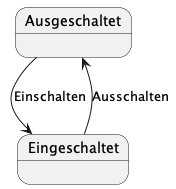
\includegraphics[width=0.25\textwidth]{fig/uml/lampe.png}
  \caption{Einfache FSM Lampe}
  \label{fig:lampe}
\end{figure}
Für die Erstellung einer geeigneten RESTful API mit HATEOAS (Hypermedia as the Engine of Application State) verwenden wir die folgende Struktur:
\\\\
Zustände abbilden:
\\
Ausgeschaltet: /lamp/off\\
Eingeschaltet: /lamp/on\\
\\\\
HTTP-Verben für Zustandsübergänge:
\\
Einschalten: PUT /lamp/on\\
Ausschalten: PUT /lamp/off
\\\\
Nun werden noch die HATEOAS-Links in den API-Antworten eingebunden. Somit ergibt sich ein Beispiel für eine JSON-Antwort, wenn die Lampe ausgeschaltet ist:\\\\
\noindent\begin{minipage}{\textwidth}
\begin{lstlisting}[caption={Fallbeispiel REST - aus},captionpos=b,label={lst:rest_on}]
{
  "state": "Ausgeschaltet",
  "links": [
    {
      "rel": "self",
      "href": "/lamp/off",
      "method": "GET"
    },
    {
      "rel": "Einschalten",
      "href": "/lamp/on",
      "method": "PUT"
    }
  ]
}
\end{lstlisting}
\end{minipage}

\noindent\begin{minipage}{\textwidth}
\begin{lstlisting}[caption={Fallbeispiel REST - an},captionpos=b,label={lst:rest_an}]
{
  "state": "Eingeschaltet",
  "links": [
    {
      "rel": "self",
      "href": "/lamp/on",
      "method": "GET"
    },
    {
      "rel": "Ausschalten",
      "href": "/lamp/off",
      "method": "PUT"
    }
  ]
}
\end{lstlisting}
\end{minipage}
Die JSON-Antworten enthalten den aktuellen Zustand der Lampe und HATEOAS-Links, die den möglichen Zustandsübergängen entsprechen. Dies ermöglicht es den Clients, die API dynamisch zu erkunden und zu verwenden, ohne die zugrunde liegende Struktur der API kennen zu müssen.\\\\

Liegt die Lösung der Software-Architektur als funktionale Zerlegung in der Grundarchitektur - beispielhaft - in einer MVC Architektur vor, könnte ein Adapter die Lücke zwischen der REST Architektur und der MVC Architektur schließen. Um einen Adapter zu erstellen, können wir das Adapter-Entwurfsmuster verwenden. Im Folgenden finden Sie ein Beispiel, das den vorherigen Ansatz modifiziert, um das MVC-Muster zu integrieren:


Um das Beispiel zu vereinfachen, wurde ein Python Syntax gewählt. Zuerst erstellen wir ein Lampenmodell, das die Logik für das Ein- und Ausschalten der Lampe enthält:\\\\
\noindent\begin{minipage}{\textwidth}
\begin{lstlisting}[caption={LampModel},captionpos=b,label={lst:lamp_m}]
class LampModel:
    def __init__(self):
        self.state = "AUS"

    def toggle(self):
        if self.state == "AUS":
            self.state = "EIN"
        else:
            self.state = "AUS"

    def get_state(self):
        return self.state

\end{lstlisting}
\end{minipage}
Dann erstellen wir einen Lampen-Controller, der das Modell verwendet und die Methoden on() und off() bereitstellt:\\\\
\noindent\begin{minipage}{\textwidth}
\begin{lstlisting}[caption={LampController},captionpos=b,label={lst:lamp_c}]
class LampController:
    def __init__(self, model):
        self.model = model

    def on(self):
        if self.model.get_state() == "AUS":
            self.model.toggle()

    def off(self):
        if self.model.get_state() == "EIN":
            self.model.toggle()
\end{lstlisting}
\end{minipage}
Schließlich erstellen wir einen Adapter, der den Lampen-Controller verwendet, um die Methoden on() und off() in der REST-API zu nutzen:\\\\
%\noindent\begin{minipage}{\textwidth}
\begin{lstlisting}[caption={LampAdapter},captionpos=b,label={lst:lamp_a}]
class LampAdapter(Resource):
    def __init__(self, controller):
        self.controller = controller

    def get(self):
        response = {
            "state": self.controller.model.get_state(),
            "_links": {
                "self": {"href": "/lamp"},
                "on": {"href": "/lamp/on"},
                "off": {"href": "/lamp/off"},
            }
        }
        return jsonify(response)

    def put(self):
        action = request.form.get("action")

        if action == "on":
            self.controller.on()
        elif action == "off":
            self.controller.off()

        response = {
            "state": self.controller.model.get_state(),
            "_links": {
                "self": {"href": "/lamp"},
                "on": {"href": "/lamp/on"},
                "off": {"href": "/lamp/off"},
            }
        }
        return jsonify(response)
\end{lstlisting}
%\end{minipage}
Zum Schluss integrieren wir den Adapter prototypisch in die Flask-App:\\\\
%\noindent\begin{minipage}{\textwidth}
\begin{lstlisting}[caption={Lamp REST APP},captionpos=b,label={lst:lamp_r}]
from flask import Flask, jsonify, request
from flask_restful import Resource, Api

app = Flask(__name__)
api = Api(app)

lamp_model = LampModel()
lamp_controller = LampController(lamp_model)
lamp_adapter = LampAdapter(lamp_controller)

api.add_resource(lamp_adapter, "/lamp", "/lamp/toggle", "/lamp/on", "/lamp/off")

if __name__ == "__main__":
    app.run(debug=True)
\end{lstlisting}
%\end{minipage}
Der Adapter verbindet nun das REST-Design mit dem MVC-Design. Die API unterstützt das Ein- und Ausschalten der Lampe über separate Endpunkte (/lamp/on und /lamp/off). Der Adapter verwendet den Lampen-Controller, um die on()- und off()-Methoden aufzurufen und auf das Modell zuzugreifen.
\\\\
Die vorgestellte Lösung ist ein Beispiel dafür, wie man das MVC-Design (Model-View-Controller) mit RESTful-APIs kombiniert, um sauberen und wartbaren Code zu schreiben. Es ist insofern üblich, als dass es bewährte Praktiken aus Software-Designmustern und Architekturen verwendet.

Es ist wichtig zu beachten, dass es keine \enquote{Einheitslösung} gibt, die auf alle Projekte oder Situationen anwendbar ist. Die beste Lösung hängt von den spezifischen Anforderungen und Bedingungen Ihres Projekts ab. In vielen Fällen ist es jedoch sinnvoll, Designmuster wie MVC und RESTful-APIs zu verwenden, um eine klare Trennung von Verantwortlichkeiten zu erreichen und die Komplexität des Codes zu reduzieren. Dies ist nur ein Beispiel, das die Anwendung dieser Prinzipien zeigt und kann als Ausgangspunkt für die Anpassung an die Anforderungen Ihres Projekts dienen. In der Praxis müssen Sie möglicherweise verschiedene Aspekte wie Skalierbarkeit, Performance und Sicherheit berücksichtigen und auf zusätzliche Anforderungen und Herausforderungen reagieren, die sich aus der realen Anwendung ergeben.
\\\\
Dennoch, die ReSTful-API eignet sich in dem Sinne der funktionalen Zerlegung für eine Lampe, da wir eine zeitliche Kopplung mit einem zustandslosen Dienst vorfinden. Sollten wir aber eine Echtzeitanforderung an die Schaltung der Lampe über Best-Effort formulieren, oder an der Lampe noch einen Bewegungsmelder mit automatischer Aktivierung der Lampe montieren, wirkt die Lösung mit der vorgestellten RESTful API nicht mehr attraktiv. 
\\\\
Diskutierbar ist auch ein weiteres Beispiel mit einer noch loseren zeitlichen Kopplung als über RESTful API Alternativen, oder der Nutzung leichtgewichtigerer Lösungen.
Alternativen zu RESTful API können zum Beispiel sein
\begin{itemize}
\item \textbf{CoAP} (Constrained Application Protocol): CoAP ist ein leichtgewichtiges, webbasiertes Protokoll, das speziell für eingeschränkte Umgebungen und Geräte entwickelt wurde. Es basiert auf dem REST-Architekturstil und verwendet das User Datagram Protocol (UDP) statt TCP, was es für den Einsatz in Low-Power- und verlustbehafteten Netzwerken geeignet macht. CoAP unterstützt die gleichen HTTP-Methoden wie GET, POST, PUT und DELETE und bietet eine einfache Möglichkeit, Ressourcen in IoT-Anwendungen zu identifizieren und zu manipulieren.
\item \textbf{XMPP} (Extensible Messaging and Presence Protocol): XMPP ist ein offenes, XML-basiertes Protokoll, das ursprünglich für Instant Messaging und Präsenzinformationen entwickelt wurde. Es ist ein erweiterbares und flexibles Protokoll, das auch für IoT-Anwendungen verwendet werden kann. XMPP bietet eine Vielzahl von Funktionen, wie beispielsweise die Fähigkeit, Nachrichten an mehrere Empfänger zu senden, und es unterstützt die Kommunikation über verschiedene Netzwerktopologien hinweg.
\item \textbf{AMQP} (Advanced Message Queuing Protocol): AMQP ist ein offenes, binäres Messaging-Protokoll, das für die Kommunikation zwischen Anwendungen und Systemen entwickelt wurde. Es ist ein zuverlässiges und sicheres Protokoll, das verschiedene Nachrichtenaustauschmuster wie Publish-Subscribe, Punkt-zu-Punkt und Request-Reply unterstützt. Im Vergleich zu MQTT ist AMQP komplexer und bietet mehr Funktionen, was es für den Einsatz in Enterprise-Anwendungen und für den Nachrichtenaustausch in verteilten Systemen geeignet macht.
\item \textbf{DDS} (Data Distribution Service): DDS ist ein Echtzeit-Publish-Subscribe-Protokoll, das für die Verteilung und den Austausch von Daten in Hochleistungs- und Echtzeitanwendungen entwickelt wurde. Es bietet Funktionen wie Quality of Service (QoS), Filterung und Sicherheit und eignet sich besonders für Anwendungen in Industrie, Verteidigung und Luft- und Raumfahrt.
\item \textbf{OPC-UA} (OPC Unified Architecture): OPC-UA ist ein industrielles Kommunikationsprotokoll, das für den Datenaustausch zwischen industriellen Steuerungssystemen und Automatisierungsgeräten entwickelt wurde. Es ist ein plattformunabhängiges, skalierbares und sicheres Protokoll, das eine Vielzahl von Funktionen bietet, wie z. B. Informationsmodellierung, Sicherheit und Discovery.
\end{itemize}
Die Auswahl des am besten geeigneten Protokolls hängt von den spezifischen Anforderungen und Zielen des Projekts ab. Dabei sollten Faktoren wie Bandbreite, Latenz, Sicherheit, Skalierbarkeit und Netzwerkumgebung berücksichtigt werden. Eine immer größere Beliebtheit haben Message Queue Broker Protokolle, die nun in einem eigenen Kapitel diskutiert werden.  

\subsubsection{IETF Message Broker Protokolle}

AMQP, STOMP und MQTT sind alle Protokolle, die für die Nachrichtenübertragung zwischen Systemen und Geräten aus dem Kontext der IETF verwendet werden können. Sie sind auf unterschiedliche Weise gestaltet und bieten unterschiedliche Funktionen, aber sie haben auch einige Gemeinsamkeiten. Alle drei Protokolle sind zustandsbasiert, was bedeutet, dass sie eine Verbindung zwischen dem Client und dem Broker herstellen und aufrechterhalten, um die Nachrichtenübertragung zu erleichtern. Sie verwenden alle einen Broker als Vermittler zwischen den Clients, um die Nachrichtenübertragung zu koordinieren und zu verwalten.
Alle drei Protokolle unterstützen eine Vielzahl von Anwendungen und können in verschiedenen Umgebungen wie IoT, Messaging-Systemen und anderen Anwendungsfällen eingesetzt werden.
Sie bieten alle eine hohe Skalierbarkeit, um die Anforderungen an die Nachrichtenübertragung in großen Systemen und Netzwerken zu erfüllen. 
\\\\
\textbf{AMQP}, die Abkürzung für Advanced Message Queuing Protocol, wurde als offener Ersatz für bestehende proprietäre Messaging-Middleware entwickelt. Zwei der wichtigsten Gründe für die Verwendung von AMQP sind Zuverlässigkeit und Interoperabilität. Wie der Name schon andeutet, bietet es eine breite Palette von Funktionen für das Messaging, einschließlich zuverlässiger Warteschlangen, themenbasiertem Publish-and-Subscribe-Messaging, flexiblem Routing, Transaktionen und Sicherheit. AMQP-Austausche leiten Nachrichten direkt weiter. Dies geschieht nach Themen (Topics) oder auch basierend auf Header-Informationen.

Bei einem so umfangreichen Funktionsumfang sind viele fein abgestufte Steuerungsmöglichkeiten vorhanden. Sie können den Zugriff auf Warteschlangen beschränken, ihre Tiefe verwalten und vieles mehr. Funktionen über Nachrichteneigenschaften, Anmerkungen und Header machen es zu einer guten Lösung für eine Vielzahl von Unternehmensanwendungen. Dieses Protokoll wurde für die Steigerung der Zuverlässigkeit vieler großer Unternehmensanwendungen entwickelt, die auf Messaging angewiesen sind, um Anwendungen zu integrieren und Daten innerhalb ihrer Organisation zu bewegen. AMQP ist ein binäres Protokoll, das für die Interoperabilität zwischen verschiedenen Anbietern entwickelt wurde. Wo andere Protokolle versagt haben, hat sich AMQP durchgesetzt. Unternehmen wie JP Morgan verwenden es zur Verarbeitung von 1 Milliarde Nachrichten pro Tag. Die NASA verwendet es für Nebula Cloud Computing. Google verwendet es für die komplexe Ereignisverarbeitung. Es wird in einer der weltweit größten biometrischen Datenbanken verwendet, dem indischen Aadhar-Projekt, das 1,2 Milliarden Identitäten enthält. Es wird in der Ocean Observatories Initiative verwendet - eine Architektur, die täglich 8 Terabyte an Daten sammelt. 
\\\\
\textbf{MQTT} (Message Queue Telemetry Transport) wurde ursprünglich vom IBM-Team für Pervasive Computing und dessen Arbeit mit Partnern aus der Industrie entwickelt. In den letzten Jahren wurde das Protokoll in die Open-Source-Gemeinschaft überführt, erfuhr mit dem Aufschwung mobiler Anwendungen einen beträchtlichen Popularitätszuwachs. Die Konstruktionsprinzipien und Ziele von MQTT sind viel einfacher und zielgerichteter als die von AMQP - es bietet Publish-and-Subscribe-Messaging (keine Warteschlangen, trotz des Namens) und wurde speziell für ressourcenbeschränkte Geräte und Netzwerke mit geringer Bandbreite und hoher Latenz entwickelt. Im Grunde kann es besonders in eingebetteten Systemen effektiv eingesetzt werden.

Einer der Vorteile von MQTT gegenüber vollwertigen \enquote{Enterprise Messaging}-Brokern besteht darin, dass es aufgrund seines absichtlich geringen Platzbedarfs ideal für die heutigen mobilen und sich entwickelnden Anwendungen im Stil des \enquote{Internet der Dinge} ist. Unternehmen wie Facebook verwenden es sogar als Teil ihrer mobilen Anwendungen, weil es so wenig Strom verbraucht und die Netzwerkbandbreite schont.

Einige der MQTT-basierten Broker unterstützen viele tausend gleichzeitige Geräteverbindungen. MQTT bietet drei Dienstqualitäten.

Die Stärken von MQTT sind Einfachheit (nur fünf API-Methoden), eine kompakte binäre Paket-Nutzlast (keine Nachrichteneigenschaften, komprimierte Header, viel weniger ausführlich als etwas Textbasiertes wie HTTP), und es eignet sich gut für einfache Push-Nachrichten-Szenarien wie Temperatur-Updates, Börsenticker, Öldruck-Feeds oder mobile Benachrichtigungen. Es ist auch sehr nützlich, um Maschinen miteinander zu verbinden, z. B. um ein Arduino-Gerät mit einem Webdienst über MQTT zu verbinden.
\\\\
\textbf{STOMP} (Simple/Streaming Text Oriented Messaging Protocol) ist das einzige dieser drei Protokolle, das textbasiert ist und damit in Bezug auf sein Erscheinungsbild eher mit HTTP vergleichbar ist. Wie AMQP bietet STOMP einen Nachrichten- (oder Rahmen-) Header mit Eigenschaften und einen Rahmenkörper. Die Entwurfsprinzipien waren hier, etwas Einfaches und weitgehend Interoperables zu schaffen. So ist es beispielsweise möglich, eine Verbindung zu einem STOMP-Broker mit einem einfachen Telnet-Client herzustellen.

STOMP arbeitet jedoch nicht mit Warteschlangen und Themen, sondern verwendet eine SEND-Semantik mit einer \enquote{Ziel}-String. Der Broker muss auf etwas abbilden, das er intern versteht, wie z. B. ein Thema, eine Warteschlange oder einen Austausch. Die Verbraucher SUBSCRIBEN dann zu diesen Zielen. Da diese Ziele in der Spezifikation nicht vorgeschrieben sind, können verschiedene Broker unterschiedliche Arten von Zielen unterstützen. Daher ist es nicht immer einfach, Code zwischen Brokern zu portieren.

STOMP ist jedoch einfach und leichtgewichtig (wenn auch etwas langatmig auf dem Draht), mit einer breiten Palette von Sprachbindungen. Es bietet auch einige transaktionale Semantiken. Eines der interessantesten Beispiele ist RabbitMQ Web Stomp, mit dem Sie Nachrichten in einem Browser über Websockets bereitstellen können. Dies eröffnet einige interessante Möglichkeiten, z. B. die Aktualisierung eines Browsers, einer mobilen Anwendung oder einer Maschine in Echtzeit mit allen Arten von Informationen.

\subsubsection{Message Broker}
Das Skript legt im weiteren weniger Wert auf STOMP oder AMQP, sondern legt zunächst den Fokus auf MQTT und vergleicht es gegenüber einem proprietären Protokoll aus dem APACHE Kafka Kontext. MQTT steht für ein Beipiel bei der Unterstützung einer Vielzahl von Geräten und Apache Kafka für die Etablierung einer hohen Verarbeitung von einer Vielzahl von Transaktionen.
\\\\
MQTT (Message Queuing Telemetry Transport) und Apache Kafka sind zwei verschiedene Protokolle bzw. Systeme, die für die Kommunikation in verteilter Umgebung und für die Verarbeitung von Datenströmen entwickelt wurden. Sie haben unterschiedliche Anwendungsfälle und Eigenschaften. Hier ist eine Diskussion über die Hauptunterschiede zwischen MQTT und Kafka:
\\\\
MQTT ist wie erwähnt ein leichtgewichtiges Publish-Subscribe-Protokoll, das speziell für eingeschränkte Umgebungen und Geräte mit begrenzter Rechenleistung und Bandbreite entwickelt wurde. Apache Kafka hingegen ist ein verteiltes Streaming-System, das für die Verarbeitung großer Datenmengen und Hochdurchsatz-Workloads entwickelt wurde. Es ist ein skalierbares und fehlertolerantes System, das für die Kommunikation zwischen großen verteilten Anwendungen und für die Verarbeitung und Speicherung von Datenströmen in Echtzeit verwendet wird.
\\\\
Während MQTT für Szenarien entwickelt wurde, in denen eine geringe Latenz und geringer Bandbreitenverbrauch wichtig sind, ist Kafka für den Datenaustausch und die Verarbeitung in groß angelegten, verteilten Anwendungen und Systemen entwickelt worden.

MQTT bietet eine Quality of Service (QoS) für die Nachrichtenübertragung, die es ermöglicht, unterschiedliche Grade der Zuverlässigkeit und Garantien für die Nachrichtenübermittlung zu wählen. Auf der anderen Seite bietet Kafka starke Haltbarkeits- und Verarbeitungsgarantien, indem es eine replizierte, verteilte und fehlertolerante Architektur verwendet.
\paragraph{MQ Technologiestacks\\\\}
Auch Kafka, wenngleich sehr stark verbreitet ist in seinem Kontext - wie MQTT in seinem - ist nicht ohne Alternativen. Es gibt verschiedene alternative Technologien zu Apache Kafka, die für ähnliche Anwendungszwecke wie das Verarbeiten von Datenströmen und die Kommunikation in verteilten Systemen verwendet werden können. Einige der bekanntesten sind:
\begin{itemize}
\item Apache Pulsar: Apache Pulsar ist ein verteiltes Messaging-System und Event-Streaming-Plattform, die für hohe Skalierbarkeit, Durchsatz und niedrige Latenz entwickelt wurde. Pulsar bietet eine getrennte Architektur für Messaging und Speicherung, was es ermöglicht, den Durchsatz und die Speicherkapazität unabhängig voneinander zu skalieren. Pulsar unterstützt auch Funktionen wie Geo-Replikation und Multi-Tenancy und kann als Alternative zu Kafka für Anwendungsfälle in verteilten Systemen und Echtzeit-Datenverarbeitung verwendet werden.
\item NATS Streaming: NATS Streaming ist ein leichtgewichtiges, hochleistungsfähiges Messaging-System, das auf dem NATS-Core-Protokoll aufbaut und zusätzliche Funktionen für die Verarbeitung von Datenströmen bereitstellt. Es bietet Funktionen wie At-least-once-Delivery, Nachrichten-Acknowledgements und Nachrichten-Historie. NATS Streaming ist für seine Einfachheit und geringe Latenz bekannt und kann für Anwendungsfälle verwendet werden, in denen schnelle Nachrichtenübermittlung und Echtzeit-Verarbeitung erforderlich sind.
\item Amazon Kinesis: Amazon Kinesis ist ein vollständig verwalteter Streaming-Datendienst, der von AWS bereitgestellt wird. Kinesis ermöglicht das Sammeln, Verarbeiten und Analysieren von Echtzeit-Datenströmen und bietet Funktionen wie skalierbare Dateneingabe und automatische Skalierung. Kinesis ist gut in das AWS-Ökosystem integriert und kann für Anwendungsfälle verwendet werden, in denen Echtzeit-Datenverarbeitung, -analyse und -überwachung erforderlich sind.
\item Google Cloud Pub/Sub: Google Cloud Pub/Sub ist ein Messaging- und Event-Streaming-Dienst, der von Google Cloud bereitgestellt wird. Pub/Sub ermöglicht die asynchrone Kommunikation zwischen verteilten Systemen und unterstützt Publish-Subscribe- und Point-to-Point-Messaging-Muster. Es ist gut in das Google Cloud-Ökosystem integriert und bietet Funktionen wie At-least-once-Delivery und automatische Skalierung.
\end{itemize}

Tatsächlich sind in dieser Aufzählung Technologien und Protokolle vermischt, die für Messaging und Datenverarbeitung verwendet werden. Der Grund dafür ist, dass in vielen Anwendungsfällen wie verteilten Systemen und Echtzeit-Datenverarbeitung, die Technologien und Protokolle eng miteinander verknüpft sind und oft zusammen verwendet werden, um bestimmte Funktionen zu erreichen und somit kaum mehr zwischen dem Protokoll und der technologischen Umsetzung unterschieden wird. Dies trifft nicht zuletzt sogar für Kafka zu. 

Apache Kafka ist sowohl ein Protokoll als auch eine Technologie, die auf dem Protokoll basiert. Es ist ein Messaging- und Streaming-System, das auf seinem eigenen Protokoll aufbaut. Somit wurde - zum besseren Verständnis - in der Aufzählung nur versucht, alternative Technologien und Protokolle zu nennen, die auch ähnliche Anwendungsfälle wie Kafka abdecken können. Es ist jedoch wichtig, zwischen den Protokollen und den Technologien, die diese Protokolle implementieren, zu unterscheiden. Dies ist aber besser am Beispiel MQTT diskutiert.
\\\\
Gerade die Vielzahl der Umsetzung von Message Broker mit MQTT Unterstützung können selbst den geneigtesten Leser irritiert zurück lassen\footnote{\url{https://github.com/hobbyquaker/awesome-mqtt}}. Aus diesem sehr großen Kontext, können beispielhaft RabbitMQ und ZeroMQ genannt werden. RabbitMQ, ZeroMQ und andere Messaging-Lösungen bieten unterschiedliche Funktionen und Eigenschaften, die sie für verschiedene Anwendungsfälle und Umgebungen geeignet machen. Die Vielzahl von Message-Broker-Implementierungen existiert, weil es eine breite Palette von Anforderungen und Szenarien in verteilten Systemen und Echtzeit-Kommunikation gibt, die von verschiedenen Lösungen besser oder schlechter abgedeckt werden können.
\\\\
RabbitMQ ist ein Open-Source-Message-Broker, der neben dem MQTT auch das Advanced Message Queuing Protocol (AMQP) implementiert. Es unterstützt verschiedene Messaging-Szenarien wie Publish-Subscribe, Point-to-Point und Request-Reply. RabbitMQ ist für seine Robustheit, Zuverlässigkeit und Skalierbarkeit bekannt und eignet sich für Enterprise-Anwendungen und für den Einsatz in verteilten Systemen.
\\\\
ZeroMQ hingegen ist eine leichtgewichtige Messaging-Bibliothek, die für hohe Leistung und geringe Latenz optimiert ist. Im Gegensatz zu RabbitMQ, das als zentralisierter Broker fungiert, ist ZeroMQ brokerlos und ermöglicht den direkten Austausch von Nachrichten zwischen Anwendungen oder Prozessen. ZeroMQ bietet verschiedene Kommunikationsmuster wie Publish-Subscribe, Request-Reply und Pipeline. Es eignet sich für Anwendungsfälle, in denen schnelle Kommunikation, geringe Latenz und einfache Skalierbarkeit erforderlich sind.
\\\\
Wichtig ist aber zu verstehen, das bei der Vielzahl der Angebote die Grundarchitektur immer sehr ähnlich ist, das folgende Kapitel wird es exemplarisch diskutieren.

\subsubsection{Message Broker Architektur}

Die Wahl der richtigen Messaging-Lösung hängt von Faktoren wie Skalierbarkeit, Latenz, Zuverlässigkeit, Kommunikationsmuster und Integration in bestehende Infrastrukturen ab. Die Vielzahl von Message-Broker-Implementierungen ermöglicht es Entwicklern, die beste Lösung für ihre Anwendungsfälle auszuwählen, indem sie die spezifischen Anforderungen ihrer Projekte und die Eigenschaften der verfügbaren Messaging-Lösungen berücksichtigen. Durch das Verständnis der Unterschiede zwischen diesen Lösungen können Entwickler fundierte Entscheidungen über die Auswahl der richtigen Messaging-Technologie für ihre Projekte treffen. Das Bauchgefühl ist hier keine gute Entscheidungsgrundlage. 
\\\\
In dem bisherigen Text sind aus Sicht des Autors die neun wichtigsten - aufgrund ihrer Marktverbreitung und Popularität - Message Broker genannt worden, zur Vervollständigung einer - wenngleich nicht die - Top 10 kann noch die IBM MQ (früher WebSphere MQ) genannt werden. Ein proprietärer Message-Broker von IBM, der für seine Zuverlässigkeit, Sicherheit und Integration in IBM-Systeme und andere Enterprise-Anwendungen bekannt ist.
\\\\
Bei IBM MQ handelt es sich um einen Middleware-Service, der eine asynchrone und zuverlässige Nachrichtenübermittlung zwischen den Systemen gewährleistet und diese Eigenschaft mit den meisten der hier genannten Systemen teilt. Hier lohnt sich in der Diskussion insbesondere ein Blick auf die internen Komponenten, dass diese nicht selten und dabei nicht zu Letzt von \cite{tanenbaum2017distributed} als Referenz herangezogen werden.
\\\\
Die innere Architektur von IBM MQ besteht aus mehreren Komponenten, die zusammenarbeiten, um eine zuverlässige und sichere Nachrichtenübermittlung zu gewährleisten:

\begin{itemize}
\item Message Queues: IBM MQ verwendet Warteschlangen, um Nachrichten zwischen den Systemen zu übermitteln. Die Anwendungen senden und empfangen Nachrichten über diese Warteschlangen, die als Puffer für Nachrichten dienen. Dadurch können Anwendungen unabhängig voneinander arbeiten und Systemausfälle abfedern, ohne dass Nachrichten verloren gehen.
\item Message Channel Agents (MCAs): MCAs sind verantwortlich für die Übertragung von Nachrichten zwischen den MQ-Servern (auch als Queue-Managern bezeichnet). Sie sorgen dafür, dass die Nachrichten sicher und zuverlässig zwischen den Systemen übertragen werden, indem sie Funktionen wie Verschlüsselung, Komprimierung und Nachrichten-Acknowledgements bereitstellen.
\item Queue Manager: Der Queue Manager ist das Herzstück von IBM MQ und verwaltet die Warteschlangen und die Nachrichtenübermittlung. Er ist dafür verantwortlich, die Nachrichten zwischen den Warteschlangen zu übertragen, die Nachrichtenpersistenz sicherzustellen und die Verarbeitung von Nachrichten zu steuern.
\item Clients: IBM MQ Clients sind Anwendungen, die auf Client-Systemen ausgeführt werden und mit dem IBM MQ Server über das Message Queue Interface (MQI) kommunizieren. Die Clients senden und empfangen Nachrichten über die Warteschlangen und können in verschiedenen Programmiersprachen geschrieben sein.
\end{itemize}

Unter der Haube wird das Publish-Subscribe-Pattern in der Regel durch eine Message Queue implementiert. Der Publisher sendet die Nachrichten an eine Queue, die für die Empfänger zugänglich ist. Die Empfänger können sich auf die Queue abonnieren, um die Nachrichten zu erhalten, die vom Publisher gesendet werden. Sobald eine neue Nachricht in der Queue eintrifft, wird sie an alle Abonnenten der Queue verteilt.
\\\\
Das Pub-Sub-Muster kann auch durch andere Mechanismen implementiert werden, wie z.B. durch die Verwendung von Topics oder Channels. In diesem Fall sendet der Publisher die Nachrichten an einen bestimmten Topic oder Channel, und die Empfänger abonnieren den entsprechenden Topic oder Channel, um die Nachrichten zu erhalten.
\\\\
Es gibt verschiedene Möglichkeiten, die Priorisierung von Nachrichten in einer Publish-Subscribe-Architektur umzusetzen.

Eine Möglichkeit ist die Verwendung von Prioritätsniveaus, bei der jede Nachricht eine Priorität zugewiesen wird. Die Prioritäten können je nach der Bedeutung der Nachricht oder dem Zeitrahmen, innerhalb dessen sie verarbeitet werden muss, variiert werden. Die Message Queue kann dann so konfiguriert werden, dass sie die höher priorisierten Nachrichten zuerst verarbeitet.

Eine weitere Möglichkeit ist die Verwendung von Routing-Regeln, bei der die Nachrichten basierend auf bestimmten Kriterien an bestimmte Empfänger weitergeleitet werden. Diese Kriterien können beispielsweise der Inhalt der Nachricht, der Sender oder der Empfänger sein. Durch die Verwendung von Routing-Regeln können Nachrichten an die richtigen Empfänger weitergeleitet werden, basierend auf ihrer Priorität.

Es gibt auch spezialisierte Software-Tools, die die Priorisierung von Nachrichten in Publish-Subscribe-Systemen unterstützen. Zum Beispiel kann Apache Kafka Konfigurationen bereitstellen, um die Reihenfolge der Verarbeitung von Nachrichten zu steuern und das Verarbeiten von höher priorisierten Nachrichten zu priorisieren.

\subsubsection{Fehlersemantik}

Neben der Priorisierung ist auch die Qualität der Dienstleistung (QoS) entscheidend für den Erfolg, insbesondere die damit verbundenen Fehlersemantik. Dies soll am Beispiel von MQTT diskutiert werden.
MQTT unterstützt drei QoS-Levels (0, 1 und 2), die unterschiedliche Garantien bezüglich der Nachrichtenzustellung bieten, die im Folgenden  auch allgemeine diskutiert werden sollen. 
\begin{itemize}
\item QoS 0 - Maybe: QoS 0 bedeutet, dass Nachrichten nach Best Effort QoS zugestellt werden. Es gibt keine Garantie für die Zustellung, und es ist möglich, dass Nachrichten verloren gehen oder dupliziert werden. Dieses Level ist ideal für Anwendungsfälle, bei denen Datenverlust oder Duplikate tolerierbar sind, z. B. bei Sensordaten, die kontinuierlich übertragen werden. Die Fehlersemantik in diesem Level ist \enquote{maybe} (vielleicht), da die Zustellung nicht garantiert ist.
\item QoS 1 - At-least-once (Mindestens einmal):
Bei QoS 1 wird sichergestellt, dass Nachrichten mindestens einmal zugestellt werden. Dies bedeutet, dass der Sender die Nachricht wiederholt sendet, bis eine Empfangsbestätigung (ACK) vom Empfänger erhalten wird. Dieses Level ist ideal für Anwendungsfälle, bei denen die Zustellung wichtiger ist, und Datenverlust vermieden werden muss. Die Fehlersemantik in diesem Level ist \enquote{at-least-once"}(mindestens einmal), da Nachrichten möglicherweise mehrmals zugestellt werden.
\item QoS 2 - Exactly-once (Genau einmal):
QoS 2 garantiert, dass Nachrichten genau einmal zugestellt werden. Dieses Level stellt sicher, dass keine Nachrichten verloren gehen oder dupliziert werden. Um dies zu erreichen, wird ein Vier-Wege-Handshake-Verfahren zwischen Sender und Empfänger durchgeführt, das den Nachrichtenaustausch koordiniert. Dieses Level ist ideal für Anwendungsfälle, bei denen sowohl Datenverlust als auch Duplikate unzulässig sind, z. B. bei Steuerungs- oder Transaktionsdaten. Die Fehlersemantik in diesem Level ist \enquote{exactly-once} (genau einmal), da Nachrichten garantiert nur einmal zugestellt werden.
\end{itemize}

Die Fehlersemantiken at-least-once, at-most-once und exactly-once beziehen sich auf die Garantien, die ein Kommunikationssystem oder ein Protokoll hinsichtlich der Zustellung von Nachrichten bietet und können noch allgemein gesprochen um maybe erweitert werden. Sie haben einen signifikanten Einfluss auf die Architektur und das Verhalten von Systemen in Bezug auf Stateless- oder Stateful-Charakteristiken, Geschwindigkeit und Blockierungen:
\begin{itemize}
\item  Maybe (Vielleicht): Die maybe-Fehlersemantik bedeutet, dass die Nachrichtenzustellung nicht garantiert ist und Nachrichten möglicherweise verloren gehen können. Systeme, die diese Semantik verwenden, sind in der Regel stateless, da sie keine Informationen über den Zustand der Nachrichtenübermittlung speichern. Die Geschwindigkeit ist in der Regel hoch, da es keine zusätzlichen Schritte oder Wiederholungen zur Sicherstellung der Zustellung gibt. Da keine Blockierungen aufgrund von Zustellungsbestätigungen oder wiederholten Nachrichtenübermittlungen auftreten, ist die Kommunikation in solchen Systemen meist reibungslos.
\item At-most-once (Höchstens einmal): Die at-most-once-Fehlersemantik stellt sicher, dass Nachrichten höchstens einmal zugestellt werden. Ähnlich wie bei der maybe-Semantik sind Systeme, die diese Semantik verwenden, in der Regel stateless und schneller, da sie keine zusätzlichen Schritte zur Überprüfung der Nachrichtenzustellung durchführen. Diese Systeme können jedoch Nachrichten verlieren, sind aber vor Duplikaten geschützt. Blockierungen sind minimal, da keine Zustellungsbestätigungen erwartet werden.
\item At-least-once (Mindestens einmal): Die at-least-once-Fehlersemantik garantiert, dass Nachrichten mindestens einmal zugestellt werden. Systeme, die diese Semantik verwenden, sind in der Regel stateful, da sie den Zustand von Nachrichtenübermittlungen und Bestätigungen speichern müssen. Die Geschwindigkeit dieser Systeme kann aufgrund der zusätzlichen Schritte, wie dem Warten auf Empfangsbestätigungen (ACKs) und möglichen Wiederholungen, beeinträchtigt werden. Blockierungen können auftreten, wenn ein System auf Zustellungsbestätigungen wartet oder wiederholte Nachrichtenübermittlungen durchführt.
\item Exactly-once (Genau einmal): Die exactly-once-Fehlersemantik garantiert, dass Nachrichten genau einmal zugestellt werden. Systeme, die diese Semantik verwenden, sind stateful, da sie den Zustand von Nachrichtenübermittlungen, Bestätigungen und zusätzlichen Handshakes verwalten müssen. Die Geschwindigkeit dieser Systeme ist im Vergleich zu den anderen Semantiken am niedrigsten, da mehr Schritte und Kommunikationsaustausch erforderlich sind, um die exakte Zustellung zu gewährleisten. Blockierungen sind häufiger, da Systeme auf Handshakes und Bestätigungen warten, um den Nachrichtenübermittlungsprozess abzuschließen.
\end{itemize}
In verteilten Systemen ist die Exactly-Once-Fehlersemantik (auch bekannt als \enquote{Exactly Once Delivery} oder \enquote{Exactly Once Processing}) ein wichtiges Konzept, bei dem eine Nachricht genau einmal erfolgreich verarbeitet wird. Die Idee ist, dass Daten weder verloren gehen noch doppelt verarbeitet werden. In der Praxis ist die Exactly-Once-Fehlersemantik im eigentlichen Sinne jedoch unmöglich, da verteilte Systeme immer von Unsicherheiten und Unvorhersehbarkeiten betroffen sind.

Einige der Hauptgründe, warum die Exactly-Once-Fehlersemantik im eigentlichen Sinne unmöglich ist, sind:
\begin{itemize}
\item Zwei-Generäle-Problem: Das ist ein bekanntes Problem in der Informatik, das zeigt, dass es in verteilten Systemen keine Garantie dafür geben kann, dass zwei Parteien zuverlässig zu einer Übereinkunft kommen, wenn es Unsicherheiten bei der Kommunikation gibt (z.B. Nachrichtenverlust). Dies wird im folgenden Text auch nochmals intensiver diskutiert.
\item Unzuverlässige Kommunikation: Netzwerke können unzuverlässig sein, und es ist möglich, dass Nachrichten verloren gehen, beschädigt oder verzögert werden. Dies erschwert die Implementierung einer Exactly-Once-Fehlersemantik.
\item Unvorhersehbare Systemausfälle: Verteilte Systeme sind anfällig für Hardware- oder Softwareausfälle. Es ist schwierig, eine Exactly-Once-Fehlersemantik zu gewährleisten, wenn man nicht genau wissen kann, welche Komponenten ausfallen und wann dies geschehen könnte.
\end{itemize}
Trotz dieser Herausforderungen gibt es Protokolle wie MQTT (Message Queuing Telemetry Transport), die eine Exactly-Once-Fehlersemantik versprechen. Dies wird durch die Implementierung eines Mechanismus zur Kontrolle der Nachrichtenübermittlung erreicht. Es ist wichtig zu betonen, dass MQTT eine Annäherung an die Exactly-Once-Fehlersemantik bietet und in den Definitionen unterschieden wird zwischen  \textbf{message delivery} und \enquote{message processing}.\footnote{\url{https://exactly-once.github.io/posts/exactly-once-delivery/}}

\paragraph{Zwei-Generäle-Problem \\\\}
Das grundsätzliche Problem kann mit den Zwei-Generäle-Problem argumentiert werden. Das Two Generals' Problem, auch bekannt als das Byzantinische Generäle Problem, ist ein klassisches Problem in der Informatik und Kommunikationstheorie, dass sich mit der Frage der Koordination und Vertrauensbildung zwischen zwei Parteien befasst, die über einen unzuverlässigen Kommunikationskanal kommunizieren.
\\\\
Stellen Sie sich vor, es gibt zwei Generäle, General A und General B, die jeweils eine Armee kommandieren. Sie planen, eine feindliche Stadt anzugreifen und müssen sich auf den genauen Zeitpunkt des Angriffs einigen. Sie sind jedoch räumlich getrennt und können nur über Boten kommunizieren, die Nachrichten zwischen ihnen hin- und hertragen. Das Problem ist, dass der Kommunikationsweg durch das feindliche Gebiet führt und es eine Chance gibt, dass Boten abgefangen und ihre Nachrichten verloren gehen.

Um den Angriff erfolgreich durchzuführen, müssen sich beide Generäle auf den gleichen Zeitpunkt einigen und sicher sein, dass der andere General die Nachricht empfangen hat und mit dem Plan einverstanden ist. Wenn einer der Generäle angreift, während der andere sich zurückhält, wird der Angriff fehlschlagen und beide Armeen werden vermutlich besiegt werden.

Nehmen wir an, General A entscheidet sich für einen Angriffszeitpunkt und sendet einen Boten zu General B, um ihn über den Plan zu informieren. Es gibt jedoch keine Garantie, dass der Bote General B erreicht. Selbst wenn der Bote General B erreicht, wie kann General A sicher sein, dass die Nachricht erfolgreich zugestellt wurde?

Um dies zu bestätigen, könnte General B einen Boten zurückschicken, um zu bestätigen, dass er die Nachricht erhalten hat und mit dem Angriffszeitpunkt einverstanden ist. Aber was, wenn dieser bestätigende Bote verloren geht? Dann wird General A nicht wissen, ob General B die ursprüngliche Nachricht erhalten hat, und der Angriff wird gefährdet sein.

Das Two Generals' Problem zeigt, dass es in solchen Szenarien unmöglich ist, eine absolute Gewissheit der Koordination und Übereinstimmung zwischen den beiden Parteien zu erreichen, wenn der Kommunikationskanal unzuverlässig ist. Dieses Problem ist relevant für die Informatik, insbesondere in verteilten Systemen und Netzwerken, bei denen Kommunikationskanäle nicht immer zuverlässig sind und Knoten möglicherweise nicht vertrauenswürdig sind.
\\\\
In der Praxis verwenden verteilte Systeme und Netzwerke verschiedene Techniken, um den Grad der Koordination und Konsistenz zu erhöhen, wie z. B. Konsensalgorithmen (z. B. Paxos oder Raft) oder fehlertolerante Protokolle. Diese Protokolle werden noch in einem späteren Kapitel genauer diskutiert. wie es auch sei, diese Lösungen bieten jedoch auch keine absolute Garantie, sondern erhöhen lediglich die Wahrscheinlichkeit einer erfolgreichen Kommunikation und Koordination.

\paragraph{Exactly-Once-Fehlersemantik mit MQTT\\\\}

Es ist schwierig, eine exakte Wahrscheinlichkeitsberechnung für das Auftreten eines Fehlers bei der Exactly-Once-Fehlersemantik mit MQTT QoS 2 anzugeben, da dies von vielen Faktoren abhängt, wie zum Beispiel der Zuverlässigkeit des Netzwerks, der verwendeten Hardware und Software, sowie von Umweltbedingungen. Stattdessen können wir eine grobe Schätzung der Wahrscheinlichkeit solcher Fehler basierend auf einigen Annahmen diskutieren.

Angenommen, die Wahrscheinlichkeit, dass eine einzelne Nachricht während der Übertragung verloren geht, ist p (z.B. p = 0.001 oder 0.1 \%). Diese Wahrscheinlichkeit kann aufgrund von Netzwerkproblemen, Hardware- oder Softwareausfällen auftreten.

In einem QoS 2-Szenario gibt es vier Hauptnachrichten, die zwischen Sender und Empfänger (bzw. Broker) ausgetauscht werden: PUBLISH, PUBREC, PUBREL und PUBCOMP. Für den Exactly-Once-Fehlersemantik-Fehler muss eine dieser Nachrichten verloren gehen, während gleichzeitig der Wiederholungsmechanismus von MQTT versagt.

Die Wahrscheinlichkeit, dass eine dieser vier Nachrichten verloren geht, kann mit der Formel $1 - (1 - p)^4$ berechnet werden, da wir annehmen, dass die Wahrscheinlichkeiten unabhängig voneinander sind.
\\\\
Für p = 0,001 (0,1 \%) erhalten wir:
\\\\
$1 - (1 - 0.001)^4 \approx 0.00397$ oder $0.397 \%$
\\\\
Die Wahrscheinlichkeit, dass eine der vier Hauptnachrichten verloren geht, beträgt also etwa 0.397 \%. Dies ist jedoch noch nicht die endgültige Wahrscheinlichkeit für das Versagen der Exactly-Once-Fehlersemantik, da wir auch den Wiederholungsmechanismus von MQTT berücksichtigen müssen.

Angenommen, der Wiederholungsmechanismus funktioniert mit einer Zuverlässigkeit von q (z.B. q = 0.999 oder 99.9 \%). Die Wahrscheinlichkeit, dass der Wiederholungsmechanismus ebenfalls versagt, beträgt (1 - q).

Die kombinierte Wahrscheinlichkeit für das Versagen der Exactly-Once-Fehlersemantik ist dann die Wahrscheinlichkeit, dass eine der vier Nachrichten verloren geht, multipliziert mit der Wahrscheinlichkeit, dass der Wiederholungsmechanismus versagt:
\\\\
$0.00397 * (1 - 0.999) \approx 0.00000397 oder 0.000397 \%$
\\\\
In diesem Beispiel beträgt die Wahrscheinlichkeit, dass die Exactly-Once-Fehlersemantik versagt, etwa 0.000397 \%, wenn wir die oben genannten Annahmen treffen. Es ist wichtig zu betonen, dass diese Berechnung stark von den angenommenen Wahrscheinlichkeiten p und q abhängt und in der Praxis variieren kann.

Trotzdem zeigt das Beispiel, dass die Wahrscheinlichkeit eines Versagens der Exactly-Once-Fehlersemantik in einem gut konfigurierten MQTT-System mit QoS 2 sehr gering ist, solange die Netzwerk-, Hardware- und Softwarebedingungen zuverlässig sind.

Und somit ist es erwähnenswert, dass trotz solcher Ausnahmefälle MQTT mit QoS 2 eine hohe Zuverlässigkeit bei der Nachrichtenübermittlung bietet, indem es den Nachrichtenaustausch koordiniert und den Zustand der Nachrichten beibehält. Solche Szenarien sind extrem selten, und MQTT ist in der Regel in der Lage, die Exactly-Once-Fehlersemantik erfolgreich durchzuführen. Dennoch eine 100 \%-ige Sicherheit ist es nicht, dies wird uns auch nochmal zu einem späteren Zeitpunkt begleiten. 

\paragraph{Message Broker in der Praxis\\\\}

Bei Message Brokern werden oft einige Aspekte unterschätzt, die zu Herausforderungen führen können. Hier sind einige Beispiele:

\begin{itemize}
\item Komplexität: Die Einrichtung und Konfiguration eines Message Brokers kann sehr komplex sein. Es erfordert ein tiefes Verständnis der Funktionsweise des Brokers sowie der Anforderungen der Anwendung, die ihn nutzt.
\item Ausfallsicherheit: Da Message Broker oft eine zentrale Rolle in der Architektur einnehmen, müssen sie in der Regel sehr ausfallsicher sein. Ein Ausfall des Brokers kann schwerwiegende Folgen für die gesamte Anwendung haben.
\item Skalierbarkeit: Skalierbarkeit ist ein wichtiger Aspekt von Message Brokern. Wenn die Anzahl der Nachrichten oder der Verkehr auf der Plattform zunimmt, muss der Broker in der Lage sein, diese Last zu bewältigen.
\item Leistung: Die Leistung von Message Brokern ist ein weiterer wichtiger Aspekt, der oft unterschätzt wird. Wenn die Verarbeitungsgeschwindigkeit von Nachrichten nicht ausreicht, kann dies zu Verzögerungen in der Anwendung führen.
\item Sicherheit: Message Broker müssen sicher sein, um sicherzustellen, dass vertrauliche oder sensible Informationen nicht in die falschen Hände geraten.
\item Kompatibilität: Da Message Broker in der Regel in verschiedenen Anwendungen und Systemen eingesetzt werden, muss die Kompatibilität mit anderen Systemen sichergestellt werden, um eine reibungslose Integration zu ermöglichen.
\item Wartung und Support: Die Wartung und Unterstützung von Message Brokern kann sehr zeitaufwändig sein. Es ist wichtig, sicherzustellen, dass der Broker regelmäßig gewartet und aktualisiert wird, um sicherzustellen, dass er sicher und zuverlässig bleibt.
\end{itemize}
Das führt wiederum zu neuen Geschäftsmodellen, wo die Nutzung des Message Brokers im Grunde verschenkt wird, um den Nutzer an die Service Leistungen zu binden, die im besten Fall die Nachteile des Systems auffangen. 
Ein Beispiel ist hier HiveMQ. HiveMQ ist ein kommerzielles MQTT-Messaging-System, das auf die Implementierung von IoT-Plattformen und -Anwendungen spezialisiert ist. Das Unternehmen bietet sowohl eine Cloud-basierte als auch eine On-Premises-Version seines Produkts an und generiert Einnahmen durch den Verkauf von Lizenzen und den Abschluss von Abonnements.
\\\\
Das Hauptgeschäftsmodell von HiveMQ basiert auf der Lizenzierung seiner Messaging-Plattform an Unternehmen, die diese für ihre IoT-Anwendungen nutzen möchten. Es gibt verschiedene Lizenzierungsmodelle, die je nach den Anforderungen des Kunden angepasst werden können. Dazu gehören beispielsweise Abonnements auf Jahresbasis, die je nach der Anzahl der verbundenen Geräte oder der Anzahl der Nachrichten, die über die Plattform übertragen werden, gestaffelt sind.

HiveMQ bietet auch eine kostenlose Community-Version seiner Plattform an, die jedoch weniger Funktionen und Support bietet als die kommerzielle Version. 

Wichtig für den Erfolg eines Protokolls ist wie bereits öfter angesprochen das API Design. Am Ende entscheiden die Entwickler welche Technologie eingesetzt wird. So muss man verstehen, das somit häufig bei der Diskussion um die Anbindung weniger der Dienste und  die Protokolle wie HTTP, Kafka oder MQTT im Fokus stehen, sondern vielmehr der Zugriff auf die darin kodierten Funktionen. Diesen Ansatz mag man belächeln, er hat aber leider einen hohen Praxisbezug.  
\\\\
In der bekannten Fallarchitektur soll nochmals demonstriert werden, wie einfach eine Message Broker API am Beispiel von MQTT sein kann. Es gibt drei Hauptkomponenten, die am etablierten Lampen-Fallbeispiel diskutiert werden sollen: den MQTT-Broker, den Lampen-Controller (Subscriber) und den Schalter (Publisher). Der MQTT-Broker fungiert als zentrale Kommunikationsschnittstelle und leitet Nachrichten zwischen den Clients weiter. Der Lampen-Controller und der Schalter sind MQTT-Clients, die sich mit dem Broker verbinden, um Nachrichten zu senden und zu empfangen.

Der Lampen-Controller ist ein IoT-Gerät, das die Lampe steuert. Es abonniert ein MQTT-Topic, zum Beispiel "lamp/control", und reagiert auf eingehende Nachrichten, indem es den Zustand der Lampe entsprechend ändert. Wenn der Controller eine Nachricht mit dem Inhalt \enquote{on} empfängt, schaltet er die Lampe ein, und wenn er eine Nachricht mit dem Inhalt \enquote{off} empfängt, schaltet er die Lampe aus.

Der Schalter ist ein weiteres IoT-Gerät oder eine Anwendung, die zum Steuern der Lampe verwendet wird. Wenn der Benutzer die Lampe ein- oder ausschalten möchte, sendet der Schalter eine entsprechende Nachricht (entweder \enquote{on} oder \enquote{off}) an das \enquote{lamp/control}-Topic.

Vorteile und Nachteile dieser Architektur: 
\begin{itemize}
\item Skalierbarkeit: Da das MQTT-Protokoll auf dem Publish/Subscribe-Modell basiert, können problemlos mehrere Lampen-Controller und Schalter hinzugefügt werden, ohne dass eine Änderung an der zugrunde liegenden Infrastruktur erforderlich ist.
\item Entkopplung: Die Verwendung eines zentralen Brokers entkoppelt die Lampen-Controller und Schalter voneinander, sodass sie unabhängig voneinander entwickelt, getestet und gewartet werden können.
\item Effizienz: MQTT ist ein leichtgewichtiges Protokoll, das sich gut für IoT-Anwendungen und den Einsatz in ressourcenbeschränkten Umgebungen eignet.
\item Qualität der Dienstleistung (QoS): MQTT unterstützt unterschiedliche QoS-Levels, die es ermöglichen, den Nachrichtenaustausch entsprechend den Anforderungen der Anwendung anzupassen.
\item Abhängigkeit von einem zentralen Broker: Ein zentraler Broker stellt einen Single Point of Failure dar, der die gesamte Kommunikation beeinträchtigen kann, wenn er ausfällt. Um dies zu vermeiden, können jedoch redundante Broker und Clustering-Lösungen eingesetzt werden.
\item Sicherheit: Die Sicherheit von MQTT muss durch die Implementierung von Authentifizierung, Autorisierung und Verschlüsselung (z.B. durch TLS) gewährleistet werden. Dies kann zusätzliche Komplexität und Overhead verursachen.
\item Latenz: Obwohl MQTT für Low-Bandwidth- und High-Latency-Netzwerke entwickelt wurde, kann es in einigen Situationen, insbesondere bei sehr großen oder überlasteten Netzwerken, zu Latenzproblemen kommen.
\end{itemize}

Generell ist eine Architektur mit MQTT zur Steuerung einer Lampe geeignet, wenn keine harten oder weichen Echtzeitanforderungen gestellt werden. Insbesondere wenn eine skalierbare Lösung benötigt wird, die eine große Anzahl von Lampen und Schaltern unterstützt ist MQTT RESTful APIs vorzuziehen, wenn die Infrastrukturkomponenten dies zulassen. 
Neben MQTT gibt es auch weitere Systeme die sich darauf optimiert haben Nachrichtenaustausch zwischen technischen Systemen zu realisieren. Eines ist das pub-sub Verfahren in ROS. 
\paragraph{Robot Operation System\\\\}
Robot Operating System (ROS) ist ein flexibles Framework für die Entwicklung von Software für Roboter. Es bietet eine Sammlung von Tools, Bibliotheken und Konventionen, die die Komplexität der Robotik-Entwicklung reduzieren und die Zusammenarbeit zwischen Entwicklern erleichtern. ROS ermöglicht es, modulare und wiederverwendbare Softwarekomponenten für Roboter zu erstellen, die auf verschiedenen Hardwareplattformen ausgeführt werden können.

Ein wichtiger Aspekt von ROS ist das Publish-Subscribe-Verfahren (auch bekannt als \enquote{pub-sub}), das die Kommunikation zwischen verschiedenen Softwarekomponenten (auch \enquote{Knoten} genannt) ermöglicht. Im pub-sub-Modell veröffentlichen Knoten Informationen in Form von Nachrichten auf sogenannten \enquote{Topics}. Andere Knoten, die an diesen Informationen interessiert sind, können diese Topics abonnieren und die veröffentlichten Nachrichten empfangen. Dieses Verfahren ermöglicht eine lose Kopplung zwischen den Knoten, da sie nicht direkt miteinander kommunizieren müssen und keine Kenntnis voneinander haben müssen.

Ein Beispiel für das Publish-Subscribe-Verfahren in ROS könnte ein Roboter sein, der aus verschiedenen Sensoren, Aktuatoren und Steuerungskomponenten besteht. Ein Sensor könnte seine Messdaten auf einem Topic veröffentlichen, während ein Steuerungsknoten dieses Topic abonniert, um auf Basis dieser Messdaten Entscheidungen zu treffen. Gleichzeitig kann der Steuerungsknoten Befehle auf einem anderen Topic veröffentlichen, das von den Aktuatoren abonniert wird, um den Roboter entsprechend zu steuern.
\\\\
In verteilten Systemen wie ROS ist die Synchronisation der Zeit zwischen den Knoten entscheidend, um eine konsistente und korrekte Kommunikation und Steuerung zu gewährleisten. Hier kommt das Network Time Protocol (NTP) ins Spiel. NTP ist ein Protokoll zur Synchronisation der Uhren von Computern in einem Netzwerk. Es ermöglicht es, die Systemzeit der Knoten in einem ROS-System aufeinander abzustimmen, um sicherzustellen, dass alle Knoten eine gemeinsame Zeitbasis haben.

Die Bedeutung von NTP in einem ROS-System liegt in seiner Fähigkeit, Zeitstempel für veröffentlichte Nachrichten bereitzustellen, die von anderen Knoten verwendet werden können, um die zeitliche Reihenfolge der Ereignisse zu bestimmen und möglicherweise verzögerte oder veraltete Nachrichten zu erkennen. Zeitstempel sind auch wichtig für die Koordination und Synchronisation von Aktionen zwischen verschiedenen Knoten, z. B. wenn mehrere Sensoren und Aktuatoren zusammenarbeiten müssen, um eine gemeinsame Aufgabe auszuführen. NTP werden wir im nächsten Kapitel nochmals ausführlicher behandeln. 
\\\\
ROS überwacht aber durch diese Struktur und die lose Kopplung nicht die Integrität, es werden aber Mechanismen, wie z.B. Heartbeats angeboten um dies zu realisieren.  In ROS werden Heartbeats nicht direkt vom Framework selbst implementiert, sondern sie können durch individuelle Knoten oder Pakete realisiert werden.
\\\\
Heartbeats sind essenzielle Mechanismen für die Kommunikation und Synchronisation in solchen Systemen und tragen zur Stabilität und Zuverlässigkeit bei. Im Folgenden werden verschiedene Aspekte von Heartbeats und ihre Rolle in verschiedenen Anwendungsszenarien diskutiert. 

\subsubsection{Heartbeat}

Ein Heartbeat ist ein periodisches Signal, das von einer Komponente eines verteilten Systems an andere Komponenten gesendet wird, um ihre  Verfügbarkeit und Erreichbarkeit zu signalisieren. Diese Signale dienen als Lebenszeichen, ähnlich dem menschlichen Herzschlag, und ermöglichen den Komponenten, den aktuellen Zustand des Systems zu überwachen und auf Veränderungen oder Störungen zu reagieren.
\\\\
Heartbeats in verteilten Systemen haben mehrere Funktionen, die für die Kommunikation und Synchronisation zwischen den Komponenten von Bedeutung sind:

\begin{itemize}
\item Fehlererkennung: Durch den regelmäßigen Austausch von Heartbeat-Signalen können die Komponenten eines verteilten Systems den Zustand ihrer Nachbarn überwachen. Wenn ein Heartbeat von einer Komponente für eine bestimmte Zeit nicht empfangen wird, kann dies auf einen Ausfall oder eine Fehlfunktion hindeuten. Die anderen Komponenten können dann Maßnahmen ergreifen, um den Ausfall zu beheben oder die betroffene Komponente zu ersetzen.
\item Synchronisation: In verteilten Systemen ist die Synchronisation von Prozessen und Aktionen von großer Bedeutung. Heartbeats können verwendet werden, um eine gemeinsame Zeitbasis für alle Komponenten zu etablieren, indem sie beispielsweise Zeitstempel in den gesendeten Signalen enthalten. Dies ermöglicht es den Komponenten, ihre Aktionen aufeinander abzustimmen und zeitliche Inkonsistenzen zu vermeiden.
\item Lastverteilung: Heartbeats können auch zur Überwachung der Auslastung der einzelnen Komponenten in einem verteilten System verwendet werden. Indem sie Informationen über ihre aktuelle Arbeitslast in den Heartbeat-Signalen übermitteln, können die Komponenten eine effektive Lastverteilung erreichen und sicherstellen, dass Ressourcen im System optimal genutzt werden.
\end{itemize}
Trotz ihrer weit verbreiteten Anwendung und Nützlichkeit haben Heartbeats jedoch einige Nachteile in verteilten Systemen. Zum einen erzeugen Heartbeats zusätzlichen Netzwerkverkehr, da sie in regelmäßigen Abständen zwischen den Knoten im System ausgetauscht werden müssen. In großen verteilten Systemen oder bei hoher Heartbeat-Frequenz kann dies zu einer signifikanten Belastung des Netzwerks führen, die die Leistung des gesamten Systems beeinträchtigen kann. Auch kann es aufgrund von Netzwerklatenz oder temporären Verbindungsproblemen vorkommen, dass Heartbeat-Nachrichten verspätet oder gar nicht ankommen. In solchen Fällen könnte das System fälschlicherweise annehmen, dass ein Knoten ausgefallen ist, obwohl dieser tatsächlich noch aktiv ist. Diese Fehlalarme können zu unnötigen Neustarts oder Umschaltungen in der Systemkonfiguration führen.
In sehr großen verteilten Systemen kann die Verwaltung und Überwachung von Heartbeats für alle Knoten eine Herausforderung darstellen.
Die Probleme von nicht verlässlichen Fehlerdedektoren werden zu einem späteren Zeitpunkt nochmal aufgenommen. 
\\\\
Die Skalierbarkeit von Heartbeat-basierten Überwachungssystemen kann durch die zunehmende Anzahl von Knoten und den damit verbundenen Verwaltungsaufwand beeinträchtigt werden. Weiter bieten Heartbeats nur grundlegende Informationen über den Status eines Knotens, nämlich ob er aktiv ist oder nicht. Sie liefern keine detaillierten Informationen über die Leistung oder den Zustand des Knotens. Für eine umfassendere Überwachung und Fehlerbehebung sind möglicherweise zusätzliche Mechanismen erforderlich.
Nicht zu Letzt ist die  Einrichtung und Konfiguration von Heartbeats, insbesondere in komplexen verteilten Systemen, zeitaufwändig und fehleranfällig. Außerdem erfordert die Verwendung von Heartbeats eine kontinuierliche Wartung und Anpassung der Heartbeat-Intervalle und Timeout-Werte, um eine optimale Systemleistung sicherzustellen. 
Heartbeats sind aber selten mit vielen Alternativen bestückt, sodass trotz all dieser Nachteile Heartbeats mit ergänzenden Methoden zur Überwachung der Verfügbarkeit von Knoten in verteilten Systemen eingesetzt werden. 

Im Folgenden werden verschiedene Arten von Heartbeat-Protokollen und Algorithmen vorgestellt und diskutiert, um ein tieferes Verständnis ihrer Funktionsweise und Anwendungsbereiche zu vermitteln.
\\\\
Zentralisierte Heartbeat-Protokolle sind auf eine zentrale Komponente oder einen zentralen Koordinator angewiesen, der für die Überwachung der Verfügbarkeit der Systemknoten verantwortlich ist. Diese zentrale Einheit erhält regelmäßige Statusmeldungen von den Knoten, um ihre Aktivität zu verfolgen. Im Falle eines Ausfalls oder einer nicht erhaltenen Statusmeldung von einem Knoten ergreift die zentrale Einheit entsprechende Maßnahmen, um das System zu stabilisieren. Allerdings weisen zentralisierte Heartbeat-Protokolle eine potenzielle Schwachstelle auf, da die zentrale Einheit selbst ausfallen oder überlastet sein kann, was zu einer Beeinträchtigung der Überwachungsfunktion führt.
\\\\
Ein praktisches Beispiel für ein zentralisiertes Heartbeat-Protokoll ist das Manager-Worker-Modell. In diesem Szenario gibt es einen zentralen Manager, der die Verfügbarkeit mehrerer Worker-Knoten überwacht. Die Nachrichtensequenz ist wie folgt:
\begin{enumerate}[label=(\alph*)]
\item Der Manager sendet periodisch Anfragen an die Worker-Knoten.
\item Die Worker-Knoten antworten mit Heartbeat-Nachrichten, um ihre Verfügbarkeit zu signalisieren.
\item Der Manager überwacht die empfangenen Heartbeat-Nachrichten und identifiziert ausgefallene Knoten, wenn keine Antwort innerhalb einer bestimmten Zeitspanne eintrifft.
\end{enumerate}

Im Gegensatz dazu basieren dezentralisierte Heartbeat-Protokolle auf einem peer-to-peer-Ansatz, bei dem jeder Knoten direkt mit seinen Nachbarn kommuniziert, um den Systemzustand zu überwachen. Dadurch werden Single Points of Failure vermieden, was zu einer erhöhten Fehlertoleranz und Robustheit führt. Diese Art von Protokollen ist gut geeignet für große, dynamische Systeme, bei denen Knoten häufig hinzugefügt oder entfernt werden.

Ein Beispiel für ein dezentralisiertes Heartbeat-Protokoll ist das Ring-Topologie-Modell. Die Knoten sind in einem Ring angeordnet, und jeder Knoten überwacht die Verfügbarkeit seines direkten Nachbarn. Die Nachrichtensequenz ist wie folgt:
\begin{enumerate}[label=(\alph*)]
\item Jeder Knoten sendet periodisch Heartbeat-Nachrichten an seinen direkten Nachbarn im Ring.
\item Die Knoten überwachen die empfangenen Heartbeat-Nachrichten und identifizieren ausgefallene Nachbarn, wenn keine Antwort innerhalb einer bestimmten Zeitspanne eintrifft.
\end{enumerate}

Eine weitere interessante Kategorie ist die der hierarchischen Heartbeat-Protokolle, bei denen die Knoten in einer hierarchischen Struktur organisiert sind. Die Überwachung der Verfügbarkeit erfolgt hier auf verschiedenen Ebenen, wobei übergeordnete Knoten die Verantwortung für die Überwachung einer Gruppe von untergeordneten Knoten übernehmen. Dies reduziert die Kommunikationslast, da die Anzahl der übermittelten Statusmeldungen verringert wird, und verbessert die Skalierbarkeit des Systems.

Ein praktisches Beispiel für ein hierarchisches Heartbeat-Protokoll ist ein Cluster-basiertes System. In diesem Szenario sind die Knoten in Cluster-Gruppen organisiert, wobei jeder Cluster einen Cluster-Manager hat. Die Nachrichtensequenz ist wie folgt:
\begin{enumerate}[label=(\alph*)]
\item Cluster-Manager senden periodisch Heartbeat-Anfragen an die Knoten innerhalb ihrer Cluster.
\item Die Knoten antworten mit Heartbeat-Nachrichten, um ihre Verfügbarkeit zu signalisieren.
\item Cluster-Manager überwachen die empfangenen Heartbeat-Nachrichten und identifizieren ausgefallene Knoten.
\item Cluster-Manager senden periodisch Statusberichte an einen übergeordneten Manager.
\item Der übergeordnete Manager überwacht die Statusberichte und erkennt ausgefallene Cluster-Manager.
\end{enumerate}

Gossip-basierte Heartbeat-Protokolle stellen eine weitere Alternative dar, die auf einer stochastischen Informationsverbreitung basiert. Bei diesen Protokollen teilen die Knoten ihre Statusinformationen in Form von \enquote{Gossip} oder Gerüchten mit einer begrenzten Anzahl von zufällig ausgewählten Nachbarn. Diese Nachbarn verbreiten die Informationen dann weiter, sodass das Wissen über den Systemzustand schließlich über das gesamte Netzwerk verbreitet wird. Dieses Vorgehen ermöglicht eine schnelle und effiziente Informationsverteilung, selbst in sehr großen und dynamischen Systemen, und bietet eine hohe Fehlertoleranz.

Ein praktisches Beispiel für ein Gossip-basiertes Heartbeat-Protokoll ist das SWIM-Protokoll (Scalable Weakly-consistent Infection-style Process Group Membership). In diesem Szenario verbreiten die Knoten ihre Verfügbarkeit über Gossip-Nachrichten. Die Nachrichtensequenz ist wie folgt:
\begin{enumerate}[label=(\alph*)]
\item Jeder Knoten wählt zufällig einen anderen Knoten aus und sendet ihm eine Heartbeat-Nachricht.
\item Der ausgewählte Knoten aktualisiert seine Mitgliederliste und wählt zufällig weitere Knoten aus, um die empfangene Heartbeat-Nachricht weiterzuleiten.
\item Dieser Prozess wird mehrmals wiederholt, bis die Informationen über die Verfügbarkeit der Knoten im gesamten Netzwerk verbreitet sind.
Knoten, die innerhalb einer bestimmten Zeitspanne keine Heartbeat-Nachricht von einem bestimmten Knoten erhalten, identifizieren diesen als ausgefallen und aktualisieren ihre Mitgliederliste entsprechend.
\end{enumerate}

Zentralisierte Heartbeat-Protokolle bieten eine einfache und leicht verständliche Implementierung, können jedoch bei Ausfall der zentralen Einheit anfällig sein. Dezentralisierte Heartbeat-Protokolle hingegen bieten eine höhere Fehlertoleranz durch ihren peer-to-peer-Ansatz, können jedoch unter Umständen eine erhöhte Kommunikationslast verursachen.

Hierarchische Heartbeat-Protokolle bieten eine gute Balance zwischen Skalierbarkeit und Robustheit, indem sie die Kommunikationslast über verschiedene Ebenen verteilen, während gossip-basierte Heartbeat-Protokolle die stochastische Informationsverbreitung nutzen, um eine effiziente und zuverlässige Überwachung auch in großen und dynamischen Systemen zu gewährleisten.
\\\\
Bei der Implementierung von Heartbeat-Protokollen und -Algorithmen in verteilten Systemen gibt es wichtige Aspekte zu berücksichtigen, einschließlich der Unterscheidung zwischen In-Band- und Out-of-Band-Kommunikation sowie der Priorisierung von Heartbeat-Prozessen. Darüber hinaus gibt es weitere Faktoren, die bei der Implementierung und dem Betrieb von Heartbeat-Protokollen beachtet werden müssen. Eine einzelne Betrachtung wird folgend beschrieben:

\begin{itemize} 
\item In-Band- und Out-of-Band-Kommunikation: In-Band-Kommunikation bedeutet, dass die Heartbeat-Nachrichten über den gleichen Kanal wie die reguläre Datenkommunikation im verteilten System übertragen werden. Dies kann zu einer zusätzlichen Last auf dem Kommunikationskanal führen und möglicherweise die Leistung des Systems beeinträchtigen. Um solche Probleme zu vermeiden, ist es wichtig, die Häufigkeit der Heartbeat-Nachrichten angemessen zu wählen und möglicherweise die Größe der Nachrichten zu reduzieren, um die Auswirkungen auf die reguläre Datenkommunikation zu minimieren. Out-of-Band-Kommunikation hingegen bedeutet, dass die Heartbeat-Nachrichten über separate Kanäle von der regulären Datenkommunikation übertragen werden. Dies kann dazu beitragen, die Leistungseinbußen zu vermeiden, die durch In-Band-Kommunikation verursacht werden könnten. Bei der Implementierung von Out-of-Band-Kommunikation ist es wichtig, dedizierte Kanäle oder Netzwerkverbindungen bereitzustellen, die ausschließlich für die Übertragung von Heartbeat-Nachrichten genutzt werden.
\item Priorisierung von Heartbeat-Prozessen: Die Priorisierung von Heartbeat-Prozessen ist entscheidend, um sicherzustellen, dass die Überwachung der Knotenverfügbarkeit nicht von anderen Prozessen im verteilten System beeinträchtigt wird. Es ist ratsam, die Heartbeat-Prozesse so einzustellen, dass sie unabhängig von der Last auf dem System regelmäßig ausgeführt werden. Dies kann beispielsweise durch die Verwendung von Echtzeit-Prioritäten oder durch die Zuteilung von dedizierten Ressourcen für die Heartbeat-Prozesse erreicht werden.
\item Fehlertoleranz und Wiederherstellung: Bei der Implementierung von Heartbeat-Protokollen ist es wichtig, Mechanismen zur Fehlererkennung und Wiederherstellung zu berücksichtigen, die dazu beitragen, die Stabilität und Zuverlässigkeit des Systems aufrechtzuerhalten. Dies kann beispielsweise durch redundante Kommunikationspfade, automatische Neustarts oder Datenreplikation erreicht werden.
\item Anpassungsfähigkeit: Da verteilte Systeme oft dynamisch sind und sich im Laufe der Zeit verändern, sollte die Implementierung von Heartbeat-Protokollen flexibel und anpassungsfähig sein, um Änderungen in der Systemkonfiguration oder in den Anforderungen bewältigen zu können. Es sollte ein besonderer Wert auf die Policy des Mechanismus gelegt werden. Bei der Implementierung von Heartbeat-Protokollen ist es wichtig, ein effektives Konfigurationsmanagement bereitzustellen, das die Einstellung von Parametern wie Heartbeat-Intervallen, Timeouts und anderen Konfigurationsdetails ermöglicht. Dies erleichtert die Anpassung des Systems an verschiedene Anforderungen und Betriebsumgebungen.
\item Skalierbarkeit: Bei der Implementierung von Heartbeat-Protokollen ist es wichtig, die Skalierbarkeit des Systems zu berücksichtigen. Dies beinhaltet die Fähigkeit, die Anzahl der Knoten und Ressourcen im System effektiv zu verwalten, während die Leistung und Stabilität aufrechterhalten werden. Bei der Auswahl und Implementierung von Heartbeat-Protokollen sollten Skalierungsaspekte wie Kommunikationslast, Anzahl der Knoten und deren Organisation berücksichtigt werden.
\item Sicherheit: Bei der Implementierung von Heartbeat-Protokollen ist es wichtig, Sicherheitsaspekte zu berücksichtigen, um das System vor Angriffen oder Missbrauch zu schützen. Dies kann beispielsweise durch die Verwendung von Verschlüsselung, Authentifizierung und Autorisierung bei der Übertragung von Heartbeat-Nachrichten erreicht werden.
\item Monitoring und Logging: Um die Leistung und Zuverlässigkeit von Heartbeat-Protokollen im verteilten System zu überwachen, sollten umfangreiche Monitoring- und Logging-Funktionen bereitgestellt werden. Dies ermöglicht es, Probleme frühzeitig zu erkennen und gegebenenfalls Maßnahmen zur Behebung von Problemen oder zur Verbesserung der Leistung zu ergreifen.
\end{itemize} 

Heartbeat-Protokolle und Selbstheilungskonzepte sind eng miteinander verbunden, da sie beide zur Erhaltung der Stabilität und Verfügbarkeit in verteilten Systemen beitragen. Watchdog-Patterns sind ebenfalls relevant, da sie eine Überwachungsfunktion für Systemkomponenten bieten und bei Fehlern eingreifen können. Im Folgenden wird der Zusammenhang zwischen diesen Konzepten genauer erläutert.
\\\\
Heartbeat-Protokolle können dazu genutzt werden, um automatische Wiederherstellungsmaßnahmen einzuleiten, wenn ein Knotenausfall oder eine Fehlfunktion erkannt wird. Selbstheilung in verteilten Systemen bezieht sich auf die Fähigkeit des Systems, auf Ausfälle oder Fehlfunktionen von Knoten zu reagieren und sich automatisch zu erholen, ohne dass eine manuelle Intervention erforderlich ist. Einige der Selbstheilungsstrategien umfassen Neustarts, Ressourcen-Neuzuweisungen, Datenreplikation und Neukonfiguration von Knoten. Heartbeat-Protokolle sind ein wesentlicher Bestandteil solcher Selbstheilungsmechanismen, da sie die benötigten Informationen über den Zustand der Knoten liefern und Ausfälle oder Fehlfunktionen frühzeitig erkennen.
\\\\
Watchdogs überwachen die Systemkomponenten und können bei Bedarf Korrekturmaßnahmen ergreifen, wie zum Beispiel das Neustarten eines ausgefallenen Knotens oder das Senden von Benachrichtigungen an Administratoren. In verteilten Systemen kann ein Watchdog in Kombination mit Heartbeat-Protokollen verwendet werden, um die Knotenverfügbarkeit und -leistung kontinuierlich zu überwachen. Wenn ein Knoten keine Heartbeat-Nachricht innerhalb eines festgelegten Zeitrahmens sendet oder empfängt, kann der Watchdog den Knoten als ausgefallen betrachten und entsprechende Selbstheilungsmaßnahmen einleiten.
\\\\
In der Zukunft könnten adaptive und lernende Heartbeat-Systeme eine zunehmend wichtige Rolle in verteilten Systemen spielen. Diese Systeme sind in der Lage, sich automatisch an Veränderungen in der Systemumgebung oder den Anforderungen anzupassen, um die Effizienz, Stabilität und Skalierbarkeit zu verbessern.

Ein zentraler Aspekt der zukünftigen Entwicklung von adaptiven und lernenden Heartbeat-Systemen ist die Integration von maschinellem Lernen und künstlicher Intelligenz. Indem sie maschinelles Lernen und künstliche Intelligenz einsetzen, können Heartbeat-Systeme Muster und Zusammenhänge in den gesammelten Daten erkennen und daraus lernen, um ihre Leistung und Effizienz zu optimieren. Zum Beispiel könnten sie die optimalen Heartbeat-Intervalle basierend auf der erkannten Systemlast oder der Anzahl der Knoten dynamisch anpassen.
\\\\
Ein weiterer wichtiger Aspekt der zukünftigen Entwicklung von adaptiven und lernenden Heartbeat-Systemen ist die zunehmende Vernetzung und Heterogenität von verteilten Systemen. Mit dem Aufkommen von Edge-Computing, dem Internet der Dinge (IoT) und der zunehmenden Verbreitung von Cloud-Infrastrukturen ist es entscheidend, dass Heartbeat-Systeme in der Lage sind, in solchen komplexen Umgebungen effektiv zu funktionieren. Adaptive und lernende Heartbeat-Systeme könnten dazu beitragen, die Herausforderungen dieser Umgebungen zu bewältigen, indem sie sich an unterschiedliche Kommunikationsprotokolle, Hardware-Ressourcen und Netzwerktopologien anpassen.

Schließlich könnten adaptive und lernende Heartbeat-Systeme auch von der Weiterentwicklung von Kommunikationstechnologien profitieren. Durch den Einsatz neuer Kommunikationsstandards und -protokolle, die speziell für verteilte Systeme entwickelt wurden, könnten Heartbeat-Systeme effizienter und leistungsfähiger werden. Dies würde es ihnen ermöglichen, in groß angelegten und dynamischen Umgebungen wie Cloud-Infrastrukturen und IoT-Netzwerken besser zu skalieren und zu funktionieren.

\subsubsection{Multicast}

Multicast-Verkehr ist ein grundlegendes Konzept in verteilten Systemen, das die effiziente und skalierbare Übertragung von Informationen an mehrere Empfänger gleichzeitig ermöglicht. In solchen Systemen ist es häufig erforderlich, dass ein Sender Nachrichten an eine Gruppe von Empfängern sendet, ohne dass jede Nachricht einzeln an jeden Empfänger gesendet werden muss. Der Einsatz von Multicast-Techniken kann dazu beitragen, Netzwerkressourcen zu schonen und die Kommunikationslatenz zu verringern.

Eine der gängigen Multicast-Methoden in verteilten Systemen ist das Application-Level Tree-Based Multicasting. Bei dieser Technik wird die Multicast-Kommunikation auf Anwendungsebene verwaltet, indem eine Baumstruktur verwendet wird, um Nachrichten effizient an alle Mitglieder einer Empfängergruppe zu übermitteln. Der Vorteil dieses Ansatzes besteht darin, dass er unabhängig von den zugrunde liegenden Netzwerkprotokollen und -topologien eingesetzt werden kann.
\\\\
In einem Application-Level Tree-Based Multicast-System wird eine hierarchische Struktur verwendet, um die Teilnehmer in einer Gruppe zu organisieren. Der Baum besteht aus Knoten, wobei jeder Knoten für einen Teilnehmer oder eine Gruppe von Teilnehmern verantwortlich ist. Die Nachrichten werden vom Sender an die Wurzel des Baumes gesendet und entlang der Verbindungen im Baum an die Blattknoten weitergeleitet, die die eigentlichen Empfänger repräsentieren. Jeder Knoten im Baum ist dafür verantwortlich, die Nachrichten an seine untergeordneten Knoten weiterzuleiten, bis sie alle Empfänger erreicht haben.

Ein praktisches Beispiel für den Einsatz von Application-Level Tree-Based Multicasting ist das Publish-Subscribe-Muster, das häufig in verteilten Anwendungen wie Nachrichtenverteilungssystemen oder verteilten Event-Handling-Systemen verwendet wird. In solchen Systemen abonnieren die Empfänger bestimmte Themen oder Ereignisse, an denen sie interessiert sind. Wenn ein Ereignis oder eine Nachricht veröffentlicht wird, sollte es effizient an alle Abonnenten verteilt werden.

In diesem Szenario kann Application-Level Tree-Based Multicasting eingesetzt werden, um die Nachrichtenverteilung zu optimieren. Die Teilnehmer werden in einer Baumstruktur organisiert, wobei jeder Knoten für die Weiterleitung der Nachrichten an seine untergeordneten Knoten verantwortlich ist. Dadurch wird sichergestellt, dass die Nachrichten effizient und mit minimaler Latenz an alle Abonnenten verteilt werden.

Ein weiteres Beispiel für den Einsatz von Application-Level Tree-Based Multicasting sind verteilte Multimedia-Anwendungen wie Videokonferenzen oder Live-Streaming-Dienste. In solchen Anwendungen müssen Audio- und Videoströme in Echtzeit an mehrere Teilnehmer übertragen werden. Durch den Einsatz von Application-Level Tree-Based Multicasting können die Ströme effizient an alle Teilnehmer verteilt werden, ohne dass für jeden Teilnehmer separate Verbindungen aufgebaut werden müssen. Dies führt zu einer Reduzierung des Netzwerkverkehrs und einer verbesserten Skalierbarkeit der Anwendung.
\\\\
Multicast-Techniken können auch dazu verwendet werden, um Datenbankreplikationen effizienter und skalierbarer durchzuführen. Bei der Datenbankreplikation wird der Inhalt einer Datenbank auf mehrere Server verteilt, um die Verfügbarkeit, Fehlertoleranz und Lastverteilung zu verbessern. Ein solches Verfahren, das Multicast für Datenbankreplikationen verwendet, könnte als "Multicast-basierte Datenbankreplikation" bezeichnet werden.

In einem Multicast-basierten Datenbankreplikationssystem wird die Kommunikation zwischen dem primären Server und den replizierten Datenbankinstanzen über Multicast-Nachrichten abgewickelt. Anstatt separate Nachrichten an jeden replizierten Server zu senden, sendet der primäre Server eine einzelne Multicast-Nachricht, die von allen replizierten Instanzen empfangen wird. Dadurch wird der Netzwerkverkehr reduziert und die Skalierbarkeit des Systems erhöht.

Ein Beispiel für die Verwendung von Multicast-basierter Datenbankreplikation könnte ein verteiltes E-Commerce-System sein, bei dem mehrere Server in verschiedenen geografischen Regionen eingesetzt werden, um eine hohe Verfügbarkeit und eine schnelle Antwortzeit für Kunden zu gewährleisten. In diesem Szenario wird eine zentrale Datenbank, die alle Produktinformationen und Bestellungen enthält, auf mehrere Server repliziert.

Wenn ein Update auf der primären Datenbank vorgenommen wird, beispielsweise wenn ein neues Produkt hinzugefügt oder der Lagerbestand eines bestehenden Produkts aktualisiert wird, sendet der primäre Server eine Multicast-Nachricht an alle replizierten Datenbankinstanzen. Diese Nachricht enthält die erforderlichen Informationen, um das Update auf den replizierten Instanzen durchzuführen, wie zum Beispiel die geänderten Daten und die betroffenen Tabellen oder Datensätze.

Da die Multicast-Nachricht von allen replizierten Instanzen gleichzeitig empfangen werden kann, können sie das Update parallel und nahezu in Echtzeit durchführen. Dies stellt sicher, dass alle Server stets über konsistente und aktuelle Daten verfügen und gleichzeitig die Netzwerkbelastung und Latenz reduziert wird.

Wenn bei der Verwendung von Multicast-basierter Datenbankreplikation die Daten nicht gleichzeitig von allen Empfängern empfangen werden können, können verschiedene Probleme auftreten. Ein Hauptproblem besteht darin, dass die Datenbankinstanzen in einem inkonsistenten Zustand sein können, da einige von ihnen möglicherweise aktualisierte Daten haben, während andere noch veraltete Daten verwenden.

Um dieses Problem zu bewältigen, kann ein Fehlertoleranzmechanismus in das System integriert werden. Eine mögliche Strategie zur Bewältigung von Verzögerungen oder Paketverlusten bei der Multicast-Kommunikation besteht darin, die Nutzung von Bestätigungen und Zeitüberschreitungen einzuführen. Bei dieser Strategie sendet der primäre Server eine Multicast-Nachricht an alle replizierten Instanzen und wartet auf deren Bestätigungen, um sicherzustellen, dass die Daten erfolgreich empfangen wurden. Wenn die Bestätigung innerhalb einer festgelegten Zeitüberschreitung nicht empfangen wird, kann der primäre Server die Nachricht erneut senden oder alternative Kommunikationsmethoden wie Unicast verwenden, um die betroffenen replizierten Instanzen zu aktualisieren. Dieses kann algorithmisch gelöst werden, und soll noch zu einem späteren Zeitpunkt im Kontext der logischen Uhren diskutiert werden. 

Eine weitere Möglichkeit besteht darin, eine sequenzielle Nummerierung für die Updates zu verwenden, um die Reihenfolge der Updates zu verfolgen. Auf diese Weise können die replizierten Instanzen erkennen, ob sie ein Update verpasst haben, indem sie die Sequenznummern der empfangenen Updates überprüfen. Wenn sie feststellen, dass sie ein Update verpasst haben, können sie den primären Server auffordern, das fehlende Update erneut zu senden oder die erforderlichen Daten über alternative Kommunikationskanäle abzurufen.

Es ist auch wichtig, die Robustheit des Multicast-Systems zu berücksichtigen, um sicherzustellen, dass es unter verschiedenen Netzwerkbedingungen und Ausfällen effizient funktioniert. Dies kann durch den Einsatz von Fehlererkennungs- und Wiederherstellungsmechanismen wie Heartbeat-Nachrichten, redundanter Datenübertragung oder der Verwendung von mehreren primären Servern erreicht werden.

Insgesamt ist es entscheidend, dass bei der Verwendung von Multicast-basierter Datenbankreplikation Fehlertoleranzmechanismen implementiert werden, um die Konsistenz und Integrität der replizierten Datenbanken zu gewährleisten, selbst wenn die Daten nicht gleichzeitig von allen Empfängern empfangen werden können.
\\\\
Flooding-basiertes Multicasting ist eine Technik die als Alternative zu Tree-based (Baum) Multicast verstanden werden sollte. Diese Technik dient zur Verbreitung von Informationen in verteilten Systemen, bei der Nachrichten an alle Teilnehmer im Netzwerk gesendet werden, ohne auf spezielle Routing- oder Gruppenmanagementmechanismen zurückzugreifen. Bei dieser Methode sendet der ursprüngliche Absender einer Nachricht die Informationen an alle direkt verbundenen Knoten, die diese Nachricht anschließend an alle ihre direkten Nachbarn weiterleiten, mit Ausnahme des Knotens, von dem sie die Nachricht empfangen haben. Dieser Prozess setzt sich fort, bis die Nachricht das gesamte Netzwerk erreicht hat.

Obwohl Flooding-basiertes Multicasting einfach zu implementieren ist und keine komplexen Routing-Algorithmen erfordert, kann es zu einer erheblichen Redundanz in der Nachrichtenübertragung und einer ineffizienten Nutzung der Netzwerkressourcen führen, insbesondere in größeren Netzwerken. Dennoch kann es in bestimmten Anwendungsfällen, in denen einfache und schnelle Verbreitung von Informationen wichtiger ist als die effiziente Nutzung von Netzwerkressourcen, von Vorteil sein.

Ein praktisches Beispiel für die Anwendung von Flooding-basiertem Multicasting könnte ein Sensornetzwerk sein, das zur Überwachung von Umweltbedingungen wie Temperatur, Luftfeuchtigkeit oder Luftqualität eingesetzt wird. In solchen Sensornetzwerken besteht die Hauptaufgabe darin, die von den Sensoren gesammelten Daten an eine zentrale Verarbeitungseinheit oder einen Datenaggregator zu übermitteln, der die Daten analysiert und entsprechende Aktionen auslöst.

In diesem Szenario könnte Flooding-basiertes Multicasting verwendet werden, um die Daten von den Sensoren schnell an den Datenaggregator zu übermitteln, indem die Nachrichten über das gesamte Netzwerk verbreitet werden. Da die Sensoren möglicherweise über ein großes geografisches Gebiet verteilt sind und die Netzwerktopologie dynamisch sein kann, kann Flooding-basiertes Multicasting die schnelle Verbreitung von Informationen und die einfache Anpassung an Veränderungen in der Netzwerktopologie ermöglichen.

Es ist jedoch wichtig zu beachten, dass Flooding-basiertes Multicasting möglicherweise nicht die effizienteste Lösung für alle Anwendungsfälle ist, insbesondere in größeren Netzwerken oder solchen, in denen Ressourcenbeschränkungen bestehen. In solchen Fällen können alternative Multicast-Techniken, wie zum Beispiel Baum- oder Gossip-basiertes Multicasting, besser geeignet sein, um die effiziente Nutzung von Netzwerkressourcen sicherzustellen.
\\\\
Gossip-basiertes Multicasting, auch als Epidemic Multicasting bezeichnet, ist ein Ansatz zur Nachrichtenverteilung in verteilten Systemen, der auf der Idee der epidemischen Verbreitung von Informationen basiert. Bei dieser Technik teilen die Knoten in einem Netzwerk Informationen mit einer zufällig ausgewählten Teilmenge ihrer Nachbarn, anstatt sie an alle direkt verbundenen Knoten zu senden. Diese Nachbarn wiederholen den Prozess und teilen die Informationen mit einer anderen Teilmenge ihrer Nachbarn. Im Laufe der Zeit wird die Nachricht auf diese Weise im gesamten Netzwerk verbreitet.

Gossip-basiertes Multicasting zeichnet sich durch seine Einfachheit, Skalierbarkeit und Fehlertoleranz aus. Es ist besonders gut geeignet für große und dynamische Netzwerke, in denen die Topologie häufig ändert und herkömmliche Multicast-Techniken möglicherweise nicht effizient oder robust genug sind.

Ein praktisches Beispiel für die Anwendung von Gossip-basiertem Multicasting ist ein verteiltes soziales Netzwerk, in dem Benutzer Nachrichten, Statusaktualisierungen oder Medieninhalte mit ihren Freunden und Followern teilen möchten. Angesichts der potenziell großen Anzahl von Benutzern und der dynamischen Natur der Freundschafts- oder Follower-Beziehungen kann die Verwendung von Gossip-basiertem Multicasting dazu beitragen, die Last auf den einzelnen Knoten zu verringern und die Skalierbarkeit des Systems zu erhöhen.

In diesem Szenario, wenn ein Benutzer eine Nachricht oder ein Update teilt, verwendet das System Gossip-basiertes Multicasting, um die Informationen an eine zufällig ausgewählte Teilmenge seiner Freunde oder Follower zu senden. Diese Empfänger teilen dann die Informationen mit einer Teilmenge ihrer eigenen Freunde oder Follower und so weiter. Schließlich erhalten alle Mitglieder im sozialen Netzwerk, die für das Update von Interesse sind, die Informationen, ohne dass eine vollständige Flutung des Netzwerks erforderlich ist.

Gossip-basiertes Multicasting kann jedoch auch zu einer gewissen Redundanz in der Nachrichtenübertragung führen, und es kann nicht garantiert werden, dass alle Knoten die Informationen in einer bestimmten Zeit oder überhaupt erhalten. Daher kann es notwendig sein, zusätzliche Mechanismen wie Bestätigungen, Zeitüberschreitungen oder alternative Kommunikationskanäle zu implementieren, um die Zuverlässigkeit und Konsistenz der Nachrichtenverteilung sicherzustellen.
\\\\
Die Kosten der Übertragung von Mulitcast Nachrichten darf im Allgemeinen sowieso nicht unterschätzt werden, insbesondere nicht, wenn die darunter liegende physikalische Infrastruktur nicht für die Kommunikation ausgelegt ist. Die Stretch- oder Relative Delay Penalty (RDP) ist ein wichtiges Leistungskriterium bei der Bewertung von Multicast-Kommunikationssystemen, insbesondere in Overlay-Netzwerken. Die Stretch-Metrik quantifiziert den zusätzlichen Verzögerungsaufwand, der bei der Verwendung eines bestimmten Multicast-Verteilungsschemas im Vergleich zur optimalen Übertragung über das zugrunde liegende physische Netzwerk entsteht. Sie wird oft als Verhältnis ausgedrückt und gibt an, wie viel länger der tatsächliche Übertragungsweg im Overlay-Netzwerk im Vergleich zum kürzesten Weg im physischen Netzwerk ist. Da insbesondere die Overlay-Topologie nicht unbedingt optimal an die physische Topologie angepasst ist, kann die Multicast-Kommunikation über das Overlay zu zusätzlichen Verzögerungen führen. Die Stretch-Metrik hilft dabei, den Effekt dieser zusätzlichen Verzögerungen zu quantifizieren und verschiedene Multicast-Verteilungsschemata miteinander zu vergleichen.

Um eine Beispielrechnung für die Stretch-Metrik durchzuführen, betrachten wir ein einfaches Szenario mit einem physischen Netzwerk, das aus vier Knoten besteht: A, B, C und D. Die physische Distanz zwischen den Knoten ist wie folgt:
\begin{itemize} 
\item A-B: 10 km
\item A-C: 15 km
\item A-D: 20 km
\item B-C: 5 km
\item B-D: 10 km
\item C-D: 15 km
\end{itemize} 
Nehmen wir an, wir haben ein Overlay-Netzwerk, das auf diesem physischen Netzwerk basiert, und Knoten A sendet eine Multicast-Nachricht an Knoten B, C und D. Im Idealfall würde die Nachricht die Empfänger über die kürzesten Pfade im physischen Netzwerk erreichen, d.h. A-B, A-C und A-D, mit einer Gesamtdistanz von 10 + 15 + 20 = 45 km.

Nun stellen wir uns vor, dass das Overlay-Netzwerk die Nachricht über folgende Pfade verteilt:
\begin{itemize} 
\item A-B: A-C-B (Distanz: 15 + 5 = 20 km)
\item A-C: A-B-C (Distanz: 10 + 5 = 15 km)
\item A-D: A-B-D (Distanz: 10 + 10 = 20 km)
\end{itemize} 
Die Gesamtdistanz für die Nachrichtenübertragung über das Overlay-Netzwerk beträgt 20 + 15 + 20 = 55 km. Um die Stretch-Metrik für dieses Beispiel zu berechnen, teilen wir die tatsächliche Distanz im Overlay-Netzwerk durch die optimale Distanz im physischen Netzwerk:
\\\\
Stretch = Gesamtdistanz im Overlay-Netzwerk / Gesamtdistanz im physischen Netzwerk
\\\\
Stretch = 55 km / 45 km = 1,22
\\\\
In diesem Beispiel beträgt die Stretch-Metrik 1,22, was bedeutet, dass die Nachrichtenübertragung über das Overlay-Netzwerk 22 \% länger dauert als die optimale Übertragung über das physische Netzwerk. Eine höhere Stretch-Metrik weist auf eine weniger effiziente Multicast-Kommunikation im Overlay-Netzwerk hin, während eine niedrigere Stretch-Metrik eine bessere Anpassung an das physische Netzwerk und eine effizientere Nachrichtenübertragung bedeutet.
\\\\
Es ist wichtig, die Stretch-Metrik im Kontext anderer Leistungskriterien und Anforderungen zu betrachten, wie z. B. Skalierbarkeit, Fehlertoleranz und die Komplexität der Verwaltung von Multicast-Gruppen. Bei der Auswahl oder Entwicklung eines Multicast-Verteilungsschemas für ein Overlay-Netzwerk ist es ratsam, einen ausgewogenen Ansatz zu wählen, der sowohl die Effizienz der Nachrichtenübertragung (niedrige Stretch-Metrik) als auch andere Leistungs- und Zuverlässigkeitsanforderungen berücksichtigt.

\subsubsection{Serialisierungsformate}

Serialisierungsformate spielen eine entscheidende Rolle in verteilten Systemen, da sie es ermöglichen, komplexe Datenstrukturen in eine standardisierte und kompakte Darstellung zu konvertieren, die leicht über Netzwerke übertragen und von verschiedenen Systemkomponenten verarbeitet werden kann. In den letzten Jahren haben sich mehrere Serialisierungsformate wie Protocol Buffers, MessagePack, JSON und XML etabliert, die jeweils ihre eigenen Stärken und Schwächen aufweisen. In dieser Einführung werden wir die genannten Formate diskutieren und ihre Vor- und Nachteile sowie Code-Fragmente vergleichen.
\\\\
\textbf{Protocol Buffers}, ein binäres Serialisierungsformat entwickelt von Google, zeichnet sich durch seine Kompaktheit und Leistung aus, da es sowohl eine geringe Speicher- als auch Rechenoverhead aufweist. Dank seiner statischen Typisierung und Schema-Evolution ermöglicht es einen robusten Datenaustausch und bietet eine breite Unterstützung für verschiedene Programmiersprachen. Allerdings ist das binäre Format nicht direkt lesbar oder modifizierbar und erfordert eine separate Schema-Definition.
\\\\
\textbf{JSON} ist ein textbasiertes Serialisierungsformat, das sehr weit verbreitet ist und menschenlesbar ist. Es ist einfach zu verwenden und hat eine breite Unterstützung in vielen Programmiersprachen. Allerdings sind JSON-Dateien im Vergleich zu binären Formaten wie Protocol Buffers und MessagePack größer, und die Verarbeitung kann langsamer sein.
JSON ist eine einfache und leichtgewichtige Technologie, aber es fehlt eine offizielle Schema-Sprache. JSON-Schemas sind nicht so umfassend wie XML-Schemas, und es gibt auch keinen einheitlichen Standard für JSON-Schemas. Es ist sehr einfach zu parsen, aber das Parsing kann sehr fehleranfällig sein. Fehlerhafte JSON-Dokumente können schwer zu diagnostizieren sein und möglicherweise schwerwiegende Auswirkungen auf die Anwendung haben. Weiter unterstützt es keine Kommentare, was die Lesbarkeit erschweren kann.
Dennoch, eigentlich ist JSON eine sehr einfach zu lesende und zu schreibende Technologie, die auch von Entwicklern ohne spezielle Schulung verwendet werden kann. Es ist auch sehr gut für den Einsatz in Webanwendungen geeignet.
Ein sicherer Vorteil ist das es sehr leichtgewichtig ist und es benötigt im Vergleich zu anderen Formaten wie XML oder Protocol Buffers weniger Bandbreite. Dies macht es zu einer guten Wahl für Anwendungen mit begrenzter Bandbreite.
Nicht zu unterschätzen ist das Argument, das JSON  von vielen Plattformen und Programmiersprachen unterstützt wird, was es sehr einfach macht, JSON-Daten zwischen verschiedenen Systemen auszutauschen.\\\\

Serialisierung (Python):\\
python\\
\begin{lstlisting}[caption={JSON},captionpos=b,label={lst:json}]
import json

data = {"name": "Alice", "age": 30}
serialized_data = json.dumps(data)

\end{lstlisting}
\textbf{XML} ist ein weiteres textbasiertes Serialisierungsformat, das ähnliche Vorteile wie JSON bietet, aber zusätzlich Unterstützung für Namespaces, Validierung und Transformation bietet. Die größere Flexibilität und Erweiterbarkeit geht jedoch auf Kosten von Größe und Geschwindigkeit.
XML ist sehr verbreitet und einfach zu verstehen, aber es ist auch sehr umfangreich und kann schwierig zu parsen sein. Das Parsen von großen XML-Dokumenten kann sehr viel Rechenleistung erfordern und zu Leistungsproblemen führen.
Auch ist es sehr menschenlesbar, aber die Lesbarkeit führt auch zu einem größeren Overhead. Die Tags und Attribute in XML können die Datenmenge im Vergleich zu anderen Formaten aufblähen. Die Validierung von XML kann auch problematisch sein. Wenn das Schema komplex ist, kann es schwierig sein, das XML-Dokument zu validieren, und es kann auch eine Herausforderung sein, Fehlermeldungen zu interpretieren. Auf jeden Fall ist XML eine Standard-Technologie, die von vielen Tools und Plattformen unterstützt wird. Es ist auch eine flexible und erweiterbare Sprache, die einfach anzupassen ist, um neuen Anforderungen gerecht zu werden.
Sehr gut geeignet ist XML für die Darstellung von strukturierten Daten. Durch die Verwendung von Tags und Attributen können komplexe Strukturen dargestellt werden.

Acuh bei der Integration von verschiedenen Systemen spielt es seine Stärke aus.\\\\

Serialisierung (Python):\\
\begin{lstlisting}[caption={XML},captionpos=b,label={lst:xml}]
from xml.etree.ElementTree import Element, tostring

person = Element("person")
name = Element("name")
name.text = "Alice"
age = Element("age")
age.text = "30"
person.append(name)
person.append(age)

serialized_data = tostring(person)
\end{lstlisting}
\textbf{Protocol Buffers} sind nicht so einfach zu lesen und zu schreiben wie andere Formate wie JSON oder XML. Es erfordert spezielle Kenntnisse und Schulungen, um damit arbeiten zu können. Die Validierung von Protocol Buffers kann schwierig sein, da es keine offizielle Schema-Sprache gibt. Entwickler müssen eigene Validierungsmechanismen implementieren. Die Unterstützung von Protocol Buffers ist begrenzter als die von anderen Formaten. Obwohl es von vielen Plattformen und Programmiersprachen unterstützt wird, gibt es weniger Tools und Bibliotheken, die damit arbeiten können.

Darüber hinaus sind sie sehr effizient und benötigen im Vergleich zu anderen Formaten wie JSON oder XML deutlich weniger Bandbreite. Dies macht es sehr gut geeignet für Anwendungen, die eine hohe Effizienz und Skalierbarkeit erfordern. Protocol Buffers bieten eine sehr schnelle Serialisierung und Deserialisierung von Daten. Durch die Verwendung von binären Datenstrukturen ist es in der Lage, Daten schneller zu verarbeiten als Textformate wie JSON oder XML.

Protocol Buffers sind sehr gut für die Verwendung in Anwendungen geeignet, bei denen es auf eine hohe Leistung und Geschwindigkeit ankommt, wie zum Beispiel in der Finanzbranche oder in der Wissenschaft.\\\\

Protocol Buffers:\\
.proto-Datei:\\
\begin{lstlisting}[caption={Protocol Buffers},captionpos=b,label={lst:buffers}]
syntax = "proto3";
message Person {
  string name = 1;
  int32 age = 2;
}
\end{lstlisting}
Serialisierung (Python):\\
\begin{lstlisting}[caption={Protocol Buffers (Python)},captionpos=b,label={lst:buffers_python}]
from example import person_pb2

p = person_pb2.Person(name="Alice", age=30)
serialized_data = p.SerializeToString()
\end{lstlisting}
\textbf{MessagePack} hingegen ist ein weiteres binäres Serialisierungsformat, das den Vorteil hat, noch kompakter als Protocol Buffers zu sein, und bietet auch eine hohe Geschwindigkeit bei der Serialisierung und Deserialisierung. Dennoch hat es ähnliche Nachteile wie Protocol Buffers, da es nicht direkt lesbar ist und die Unterstützung für Schema-Evolution eingeschränkt ist. Natürlich ist es nicht so bekannt wie andere Formate wie JSON oder XML, was es schwieriger machen kann, Entwickler und Tools zu finden, die damit arbeiten können. Es ist ein binäres Format und nicht so einfach zu lesen wie andere Textformate wie JSON oder XML. Es ist auch schwieriger zu validieren als Textformate.
Die Unterstützung von MessagePack ist begrenzter als die von anderen Formaten. Obwohl es von vielen Plattformen und Programmiersprachen unterstützt wird, gibt es weniger Tools und Bibliotheken, die damit arbeiten können Dennoch, es ist ein sehr kompaktes Format, das im Vergleich zu anderen Formaten wie JSON oder XML deutlich weniger Bandbreite benötigt. Dies macht es sehr gut geeignet für Anwendungen, die eine hohe Effizienz und Skalierbarkeit erfordern.
Auch die sehr schnelle Serialisierung und Deserialisierung von Daten ist ein Vorteil. Durch die Verwendung von binären Datenstrukturen ist es in der Lage, Daten schneller zu verarbeiten als Textformate wie JSON oder XML.
MessagePack ist sehr gut für die Verwendung in Echtzeit-Anwendungen geeignet, da es eine geringe Latenz und eine hohe Geschwindigkeit aufweist. Es wird oft in Anwendungen wie Spiele oder Chat-Apps verwendet, bei denen es auf eine schnelle Reaktionszeit ankommt.\\\\

Serialisierung (Python):\\
\begin{lstlisting}[caption={MessagePack},captionpos=b,label={lst:msgpack}]
import msgpack

data = {"name": "Alice", "age": 30}
serialized_data = msgpack.packb(data)
\end{lstlisting}
Jedes Format hat seine eigenen Vor- und Nachteile, und die Wahl des besten Serialisierungsformats hängt von den spezifischen Anforderungen und Einschränkungen des verteilten Systems ab, in dem es eingesetzt werden soll.
Auch im Bezug auf die Validierbarkeit gibt es Unterschiede zwischen den verschiedenen Formaten.

XML hat eine umfassende Validierungsfunktionalität durch XML-Schemas, die es ermöglichen, komplexe Datenstrukturen zu definieren und zu validieren. Dies ermöglicht eine genaue Kontrolle über die Struktur und die Inhalte der Daten.

JSON bietet keine offizielle Schema-Sprache, aber es gibt verschiedene Optionen für die Validierung von JSON-Dokumenten, wie z.B. JSON Schema oder JSON Validator. Diese Optionen sind jedoch nicht so umfassend wie XML-Schemas.

MessagePack und Protocol Buffers haben keine integrierten Validierungsfunktionen. Entwickler müssen eigene Validierungsmechanismen implementieren, um sicherzustellen, dass die empfangenen Daten den erwarteten Spezifikationen entsprechen.

\subsubsection{Pull und Push}

Push und Pull sind Strategien, die in der Kommunikation eingesetzt werden können, um Informationen zu übertragen. Bei der Push-Strategie werden Informationen aktiv an den Empfänger gesendet, während bei der Pull-Strategie der Empfänger die Initiative ergreift und die Informationen aktiv abruft.
\\\\
Um die Last zwischen Push und Pull zu teilen, können verschiedene Strategien eingesetzt werden. Eine Möglichkeit besteht darin, eine hybride Strategie zu verwenden, bei der sowohl Push- als auch Pull-Elemente kombiniert werden, um die Vorteile beider Strategien zu nutzen. So können beispielsweise wichtige Informationen automatisch an den Empfänger gesendet werden, während weniger wichtige Informationen nur auf Anfrage abgerufen werden können.

Eine weitere Möglichkeit besteht darin, zwischen Push und Pull dynamisch zu wechseln, abhängig von der aktuellen Situation. So kann beispielsweise bei einer hohen Auslastung des Netzwerks oder des Empfängers auf eine Pull-Strategie umgestellt werden, um die Last zu reduzieren. Umgekehrt kann bei einer niedrigen Auslastung auf eine Push-Strategie umgestellt werden, um die Übertragung von Informationen zu beschleunigen.

Eine weitere Strategie ist die Verwendung von Caching-Systemen, die Informationen temporär speichern und bei Bedarf bereitstellen können. Dadurch können häufig abgerufene Informationen schnell zur Verfügung gestellt werden, ohne dass sie jedes Mal neu übertragen werden müssen.
\\\\
Will man diese Strategien weiter verfeinern, kann man sich mit erweiterten Konzepten auseinandersetzen. Beispielhaft ist das Information Dissemination Model (IDM) ein Ansatz sich detailierter mit der Verteilung und Verbreitung von Informationen zu beschäftigt. Es beschreibt die verschiedenen Phasen, die bei der Übertragung von Informationen durchlaufen werden, sowie die Faktoren, die die Effektivität und Effizienz der Verbreitung beeinflussen.

Das IDM besteht aus drei Hauptphasen: Erstellung, Verbreitung und Nutzung. In der Erstellungsphase wird die Information erstellt und vorbereitet, beispielsweise durch das Verfassen eines Berichts oder die Erstellung eines Videos. In der Verbreitungsphase wird die Information dann auf verschiedene Weise verteilt, wie beispielsweise durch Veröffentlichung im Internet, Versand per E-Mail oder Verteilung von Flyern. In der Nutzungsphase schließlich wird die Information von den Nutzern verwendet und angewendet.

Das IDM berücksichtigt auch verschiedene Faktoren, die die Effektivität und Effizienz der Information Dissemination beeinflussen können. Dazu gehört die Art der Information, die Zielgruppe, die verfügbaren Ressourcen und die verwendeten Technologien. Die Wahl der richtigen Kanäle und Methoden zur Verbreitung der Information sowie die gezielte Ansprache der Zielgruppe sind wichtige Faktoren, die den Erfolg der Verbreitung beeinflussen können.

Das IDM wird häufig in der Praxis eingesetzt, um sicherzustellen, dass Informationen effektiv und effizient verbreitet werden. Es wird beispielsweise bei der Entwicklung von Marketingstrategien, der Übermittlung von Regierungsinformationen oder der Verteilung von Bildungsmaterialien verwendet. Durch eine sorgfältige Planung und Umsetzung des IDM können Organisationen sicherstellen, dass ihre Informationen effektiv verbreitet werden und von den Zielgruppen genutzt werden.
\\\\
Pull-based- und Push-based-Protokolle sind zwei unterschiedliche Methoden zur Übertragung von Daten in Computernetzwerken. Push-basierte Protokolle (auch bekannt als server-initiierte Protokolle) werden von einem Server initiiert, der aktiv Daten an den Client sendet, ohne dass der Client die Übertragung anfordert. Bei einem Push-basierten Protokoll ist es also der Server, der bestimmt, wann und welche Daten an den Client gesendet werden.

Im Gegensatz dazu werden bei Pull-basierten Protokollen (auch bekannt als client-initiierte Protokolle) die Daten vom Client angefordert, wenn sie benötigt werden. Der Client initiiert also den Datenfluss, indem er den Server auffordert, bestimmte Daten zu senden.

Beide Methoden haben Vor- und Nachteile. Push-basierte Protokolle können dazu führen, dass der Server unnötigerweise Daten an den Client sendet, was zu erhöhtem Datenverkehr und Verzögerungen führen kann. Allerdings ist dies auch eine effiziente Methode, um sicherzustellen, dass der Client stets über die aktuellsten Daten verfügt, ohne dass er jedes Mal explizit nachfragen muss.

Pull-basierte Protokolle hingegen können effizienter sein, da Daten nur dann übertragen werden, wenn der Client sie tatsächlich benötigt. Allerdings kann dies auch dazu führen, dass der Client nicht immer über die aktuellsten Daten verfügt.

Insgesamt gibt es keine allgemein beste Methode. Die Wahl zwischen Pull- oder Push-basierten Protokollen hängt von den spezifischen Anforderungen des Netzwerks und der Anwendung ab. Eine Kombination aus beiden Methoden kann ebenfalls eine effektive Lösung sein, um die Vorteile beider Ansätze zu nutzen.

Zum Beispiel kann ein Push-basiertes Protokoll effektiv sein, um sicherzustellen, dass der Client stets über die aktuellsten Daten verfügt, ohne dass er jedes Mal explizit nachfragen muss. Allerdings kann dies auch zu erhöhtem Datenverkehr und Verzögerungen führen, wenn der Server unnötigerweise Daten an den Client sendet, die der Client nicht benötigt.

Auf der anderen Seite kann ein Pull-basiertes Protokoll effizienter sein, da Daten nur dann übertragen werden, wenn der Client sie tatsächlich benötigt. Allerdings kann dies auch dazu führen, dass der Client nicht immer über die aktuellsten Daten verfügt, wenn er nicht regelmäßig die Aktualisierung anfordert.
\\\\
Multicast ist ein Verfahren, das es ermöglicht, Daten an eine Gruppe von Empfängern gleichzeitig zu übertragen. Im Vergleich zur Unicast-Übertragung, bei der Daten an einen einzelnen Empfänger gesendet werden, kann Multicast eine effizientere Nutzung des Netzwerks ermöglichen, da die Daten nur einmal gesendet werden müssen, unabhängig davon, wie viele Empfänger sie empfangen.

Ob ein Push-Protokoll besser für Multicast geeignet ist als ein Pull-Protokoll, hängt von verschiedenen Faktoren ab. Ein Push-Protokoll kann effektiv sein, wenn eine große Menge an Daten gleichzeitig an eine Gruppe von Empfängern gesendet werden soll, ohne dass diese die Übertragung aktiv anfordern müssen. Bei einem Push-Protokoll ist es der Sender, der die Übertragung initiiert und die Daten an die Empfänger sendet, ohne dass diese explizit danach fragen müssen.

Ein Pull-Protokoll hingegen würde bedeuten, dass jeder Empfänger aktiv die Übertragung anfordern müsste, um die Daten zu empfangen. Dies würde jedoch zu einem erhöhten Datenverkehr führen und könnte die Effizienz der Multicast-Übertragung beeinträchtigen.

Die Wahl des Protokolls für Multicast hängt klar von den spezifischen Anforderungen der Anwendung und des Netzwerks ab. Ein Pull-Protokoll kann effektiv sein, um die Last vom Server zu nehmen gleichzeitig an eine Gruppe von Empfängern zu senden, auch vermeidet man ein aktivies Hören der Clients, da sie selbst über den Aktualisierungszeitpunkt entscheiden können. Es ist jedoch wichtig, die Vor- und Nachteile sorgfältig abzuwägen und die beste Methode für die Anwendung zu wählen.

Die Entscheidung, ob eine Kopie der Daten oder nur die Operationen, die zu den Daten geführt haben, in einem Protokoll zur Verteilung genutzt werden sollten, hängt von verschiedenen Faktoren ab.

Die Verwendung einer Kopie der Daten hat den Vorteil, dass die Empfänger der Daten sofort auf sie zugreifen können, ohne dass sie eine spezifische Operation ausführen müssen. Dies kann in Anwendungsfällen wie der Synchronisation von Datenbanken oder der Verteilung von Dateien nützlich sein, da die Empfänger auf die vollständigen und aktuellen Daten zugreifen können, ohne dass sie sie zuerst generieren oder zusammenstellen müssen.

Auf der anderen Seite kann die Verwendung der einzelnen Operationen, die zu den Daten geführt haben, sinnvoll sein, wenn die Daten sehr groß sind oder wenn die Empfänger nur an bestimmten Teilen der Daten interessiert sind. Durch das Senden von einzelnen Operationen können die Empfänger die Daten selektiv anfordern, ohne dass sie die gesamten Daten herunterladen oder darauf zugreifen müssen.
\\\\
Ein weiterer Faktor, der berücksichtigt werden sollte, ist die Größe und Komplexität der Daten sowie die verfügbare Bandbreite. Wenn es sich um kleine Datenmengen handelt, kann es effektiver sein, eine Kopie der Daten zu senden. Bei größeren und komplexeren Daten kann es jedoch effizienter sein, nur die Operationen zu senden, die zu den Daten geführt haben.

Letztendlich hängt auch hier die Wahl der Methode von den spezifischen Anforderungen und Zielen der Anwendung ab. Es kann auch sinnvoll sein, eine Kombination aus beiden Ansätzen zu verwenden, um die Vorteile beider Methoden zu nutzen.


\subsection{Service Discovery}

Service Discovery bezeichnet den Prozess der automatischen Identifizierung und Lokalisierung von Netzwerkdiensten, die von Geräten und Anwendungen bereitgestellt werden. Diese Technik ermöglicht es, Netzwerkressourcen effizient zu verwalten und zu nutzen, indem sie eine einfache und schnelle Möglichkeit bietet, Dienste zu finden und darauf zuzugreifen. Im Laufe der Zeit hat sich Service Discovery weiterentwickelt und sich an die wachsenden Anforderungen des Internets angepasst.
\\\\
In den frühen Tagen des Internets, während der 1980er und 1990er Jahre, war die Anzahl der verfügbaren Dienste begrenzt, und sie waren größtenteils statisch. Die meisten Dienste wurden manuell konfiguriert und in zentralen Verzeichnissen wie dem Domain Name System (DNS) gespeichert. DNS war eines der ersten Service-Discovery-Systeme, dass die Zuordnung von Domainnamen zu IP-Adressen ermöglichte.
\\\\
Mit dem rasanten Wachstum des Internets und der Anzahl der angebotenen Dienste entstanden neue Herausforderungen, wie z.B. die Skalierbarkeit und das Auffinden von Diensten in verteilten Systemen. Dies führte zur Entwicklung von Technologien wie dem Service Location Protocol (SLP) und dem Simple Object Access Protocol (SOAP), die die automatische Erkennung von Diensten in Netzwerken ermöglichten.
\\\\
In jüngerer Zeit haben sich Technologien wie Microservices und Containerisierung sowie der Einsatz von Cloud Computing stark verbreitet. Diese Entwicklungen haben die Notwendigkeit einer effektiven Service-Discovery-Infrastruktur weiter verstärkt. Einige der aktuellen Ideen und Technologien sind direkt mit Produkten verwoben, die bereits Teil der Ausarbeitungen waren, teils neu hinzukommen, damit aber die Breite der Produktpalette andeuten soll.
\begin{itemize}
\item Konsul: Konsul ist eine verteilter Service-Discovery- und Konfigurationslösung von HashiCorp. Es ermöglicht die einfache Registrierung und Entdeckung von Services und bietet auch Funktionen für das Netzwerk- und Anwendungsmanagement.

\item etcd: etcd ist ein verteiltes Key-Value-Store-System, das von CoreOS entwickelt wurde. Es kann als Basis für Service-Discovery-Lösungen verwendet werden, indem es die Speicherung und den Abruf von Service-Metadaten und Konfigurationsinformationen ermöglicht.

\item Kubernetes: Kubernetes ist ein weit verbreitetes Open-Source-Container-Orchestrierungssystem, das automatische Service Discovery als integrierten Bestandteil bietet. Kubernetes ermöglicht die automatische Erkennung von Services und die Verteilung von Netzwerklasten über eine Vielzahl von Anwendungen und Diensten.

\item Istio: Istio ist eine Open-Source-Service-Mesh-Plattform, die Funktionen wie Service Discovery, Load Balancing, Zugriffskontrolle und Überwachung für Microservices bereitstellt. Istio kann in Kombination mit Kubernetes verwendet werden, um Service Discovery und Netzwerkmanagement in Container-Cluster-Umgebungen zu verbessern.

\item DNS-SD (DNS Service Discovery): DNS-SD ist eine Erweiterung des DNS, die es ermöglicht, Service Discovery in DNS-basierten Netzwerken durchzuführen. Es wird häufig in Mombination mit Multicast-DNS (mDNS) eingesetzt, um Service Discovery in lokalen Netzwerken ohne zentrale DNS-Infrastruktur zu ermöglichen. Diese Kombination wird oft unter dem Namen Zeroconf oder Bonjour (von Apple) verwendet und ist weit verbreitet in Heimnetzwerken und kleineren Unternehmensnetzwerken.

\item gRPC: gRPC ist ein Open-Source-Framework für Remote Procedure Calls (RPCs) von Google, das auf dem modernen HTTP/2-Protokoll basiert. Es ermöglicht die effiziente und schnelle Kommunikation zwischen verteilten Systemen und bietet auch Unterstützung für Service Discovery und Load Balancing.

\item Eureka: Eureka ist ein Service-Discovery-System, das von Netflix entwickelt wurde. Es ermöglicht die Registrierung und Entdeckung von Diensten in einer verteilten und elastischen Architektur, wie sie häufig in Cloud-basierten Anwendungen eingesetzt wird.

\item Apache ZooKeeper: ZooKeeper ist ein Open-Source-Verteilungssystem für die Koordination von verteilten Anwendungen. Es kann als Basis für Service-Discovery-Lösungen verwendet werden und bietet Funktionen wie verteilte Synchronisation, Konfigurationsmanagement und Gruppenmitgliedschaft.
\end{itemize}
Jedes einzelne System im Detail vorzustellen, wird den hier adressierten Fokus sprengen, daher soll nur eine Einführung in den grundsätzlichen Aufbau angeboten werden. 
Die Grundlagen von Service Discovery können in drei Hauptkomponenten unterteilt werden: Service-Registrierung, Service-Anfrage. Erweitert kann das System werden durch Lokalisierung sowie Load Balancing und Failover.
\begin{itemize}
\item Service-Registrierung: Dienste, die für andere Anwendungen und Systeme verfügbar sein sollen, müssen zunächst in einem zentralen oder verteilten Service-Register registriert werden. Die Registrierung umfasst in der Regel Informationen wie den Dienstnamen, die Netzwerkadresse, den Port und möglicherweise zusätzliche Metadaten, die zur Identifizierung und Verwendung des Dienstes erforderlich sind.
\item Service-Anfrage und Lokalisierung: Anwendungen und Systeme, die einen bestimmten Dienst nutzen möchten, stellen eine Anfrage an das Service-Register, um die erforderlichen Informationen zur Lokalisierung und Verbindung mit dem gewünschten Dienst zu erhalten. Dieser Prozess ist dynamisch, sodass Änderungen in der Verfügbarkeit und Konfiguration von Diensten ohne manuelle Eingriffe automatisch berücksichtigt werden können.
\item Load Balancing und Failover: In vielen Fällen gibt es mehrere Instanzen eines Dienstes, um hohe Verfügbarkeit und Skalierbarkeit zu gewährleisten. Service Discovery-Systeme können auch Load Balancing und Failover-Strategien implementieren, um Anfragen automatisch an die am besten geeignete Instanz eines Dienstes zu verteilen und im Falle von Ausfällen nahtlos auf verfügbare Instanzen umzuschalten.
\end{itemize}    

Grundsätzlich gibt es verschiedene Architekturen von Service Discovery.
\begin{itemize}
\item In einer zentralen Architektur sind die Service-Register und die Service-Discovery-Logik auf einem zentralen Server oder einer Gruppe von Servern konsolidiert. Anwendungen und Dienste melden sich bei diesem zentralen Server an und stellen Anfragen, um auf andere Dienste zuzugreifen. Obwohl diese Architektur einfach zu implementieren ist, kann sie in groß angelegten und dynamischen Umgebungen möglicherweise weniger skalierbar und anfällig für Single Points of Failure sein.
\item Verteilte Service-Discovery-Architektur: In einer verteilten Architektur wird die Service-Discovery-Logik über mehrere Knoten oder Instanzen in einem Netzwerk verteilt. Dies kann die Skalierbarkeit und Fehlertoleranz verbessern, indem es eine dezentrale Kontrolle über die Service-Registrierung und -Entdeckung ermöglicht. Verteilte Service-Discovery-Systeme können auf Technologien wie Konsul, etcd oder ZooKeeper basieren, die eine konsistente und zuverlässige Datenhaltung in verteilten Umgebungen gewährleisten.

\item Hierarchische Service-Discovery-Architektur: In einer hierarchischen Architektur werden Service-Discovery-Systeme in verschiedenen Ebenen organisiert, wobei jede Ebene für einen bestimmten Bereich oder eine bestimmte Domäne zuständig ist. Dies kann dazu beitragen, die Skalierbarkeit und Verwaltbarkeit in groß angelegten und verteilten Umgebungen zu verbessern, indem Dienste und Anwendungen in logische Gruppen oder Cluster eingeteilt werden. In einer solchen Architektur könnten beispielsweise regionale Service-Discovery-Instanzen für Dienste in einer bestimmten geografischen Region oder einer organisatorischen Einheit zuständig sein, während eine globale Service-Discovery-Instanz den Zugriff auf Ressourcen über mehrere Regionen hinweg ermöglicht.
\end{itemize}

Auch kann man die Architektur unterscheiden aus dem Blickwinkel der Resolution. 

\begin{itemize}
\item Client-seitige Service-Discovery-Architektur: In dieser Architektur liegt die Verantwortung für die Service-Entdeckung und das Load Balancing bei den Clients oder Anwendungen selbst. Anwendungen stellen Anfragen an das Service-Register und verwenden die erhaltenen Informationen, um direkt auf die verfügbaren Dienste zuzugreifen und gegebenenfalls das Load Balancing durchzuführen. Diese Methode ermöglicht eine hohe Flexibilität und Kontrolle, erfordert jedoch, dass die Clients über die entsprechende Logik verfügen, um Service Discovery effektiv zu handhaben.

\item Server-seitige Service-Discovery-Architektur: In einer serverseitigen Architektur wird die Service-Discovery-Logik von einem oder mehreren Servern oder Proxys verwaltet, die zwischen den Clients und den Diensten vermitteln. Die Server sind für die Anfrage von Dienstinformationen, das Load Balancing und die Weiterleitung von Anfragen an die geeigneten Dienstinstanzen verantwortlich. Diese Methode kann die Komplexität auf der Clientseite reduzieren und eine zentralisierte Verwaltung der Service-Discovery-Strategien ermöglichen.
\end{itemize}

In der Praxis kann eine Service-Discovery-Lösung eine Kombination der oben genannten Architekturen verwenden, um den spezifischen Anforderungen und Beschränkungen einer bestimmten Umgebung gerecht zu werden. Wichtig ist, die richtige Balance zwischen Skalierbarkeit, Verfügbarkeit, Flexibilität und Verwaltbarkeit zu finden, um eine effiziente und zuverlässige Service-Discovery-Infrastruktur zu schaffen.

\subsubsection{Naming}

In Service-Discovery-Systemen spielen Identifikatoren eine wichtige Rolle, um Dienste und Ressourcen eindeutig zu benennen und zu verwalten. Ein Identifikator ist ein eindeutiges Token, das verwendet wird, um auf einen bestimmten Dienst oder eine Ressource in einem verteilten System zuzugreifen. Im Gegensatz dazu ist ein Name eine menschenlesbare Bezeichnung, die zur Beschreibung oder Identifizierung eines Dienstes verwendet wird. Identifikatoren sind in der Regel technisch eindeutig, während Namen möglicherweise mehrdeutig oder nicht eindeutig sind.

Es gibt verschiedene Arten von Namensräumen, die in Service-Discovery-Systemen verwendet werden können, um Identifikatoren und Namen zu organisieren und zu strukturieren:
\begin{itemize}
\item \textbf{Flacher Namensraum}: In einem flachen Namensraum sind alle Dienste und Ressourcen in einer einzigen Ebene organisiert, ohne hierarchische Struktur. Identifikatoren und Namen müssen in diesem Fall eindeutig innerhalb des gesamten Systems sein. Ein Beispiel ist die Adressierung im Chord Netz. 
\item \textbf{Hierarchischer Namensraum}: Ein hierarchischer Namensraum organisiert Dienste und Ressourcen in einer Baumstruktur, wobei Identifikatoren und Namen innerhalb jeder Ebene eindeutig sind. Dies ermöglicht eine bessere Organisation und Verwaltung von Diensten, insbesondere in groß angelegten und verteilten Umgebungen. Beispiele für hierarchische Namensräume sind das DNS mit Subdomains und Verzeichnisdienste wie LDAP. Wobei LDAP auch gerne als hybrider Ansatz bezeichnet wird, da er neben der Hierarchie  auch Attribute zulässt. 
\item \textbf{Attributbasierter Namensraum}: In einem attributbasierten Namensraum werden Dienste und Ressourcen anhand ihrer Eigenschaften oder Attribute identifiziert und organisiert. Dies ermöglicht eine flexiblere und erweiterbare Organisation von Diensten, da neue Attribute und Eigenschaften hinzugefügt werden können, ohne die bestehende Struktur zu ändern. Ein Beispiel für einen attributbasierten Namensraum ist das Service Location Protocol (SLP), das Dienste anhand von Attributen wie Diensttyp, Standort oder Kapazität auffindet. Praxisrelevantes Beispiel: In einem attributbasierten Namensraum könnte ein E-Mail-Dienst durch Attribute wie \enquote{type=email} und \enquote{location=Europe} identifiziert werden, um Dienste basierend auf ihren Eigenschaften anstelle einer festen hierarchischen Struktur zu suchen und zu lokalisieren.
\end{itemize}
Beim Entwurf von Namensräumen für Service-Discovery-Systeme sollten verschiedene Aspekte berücksichtigt werden, um eine effiziente und effektive Lösung zu gewährleisten. Die Wahl des Namensraumdesigns hat direkte Auswirkungen auf das Laufzeitverhalten von Such-, Einfüge- und Löschoperationen. Hier sind einige wichtige Faktoren, die bei der Gestaltung von Namensräumen zu beachten sind:
\begin{itemize}
\item Eindeutigkeit: Namensräume sollten so gestaltet werden, dass Identifikatoren und Namen eindeutig sind, um Verwechslungen und Konflikte zu vermeiden. Dies ist besonders wichtig in verteilten Systemen und Umgebungen mit vielen Diensten und Ressourcen.
\item Skalierbarkeit: Das Design von Namensräumen sollte die Skalierbarkeit des Service-Discovery-Systems sowohl hinsichtlich der Anzahl der verwalteten Dienste als auch der Anzahl der Anfragen unterstützen. Hierarchische und attributbasierte Namensräume können dazu beitragen, die Skalierbarkeit zu verbessern, indem sie eine bessere Organisation und Gruppierung von Diensten ermöglichen.
\item Flexibilität: Namensräume sollten flexibel genug sein, um Änderungen in der Anwendung oder Umgebung, wie z.B. das Hinzufügen oder Entfernen von Diensten und Ressourcen, ohne große Auswirkungen auf das System zu bewältigen. Attributbasierte Namensräume bieten in dieser Hinsicht eine hohe Flexibilität, da sie es ermöglichen, Dienste basierend auf ihren Eigenschaften und Attributen zu suchen, ohne eine feste hierarchische Struktur.
\item Einfachheit: Namensräume sollten einfach und leicht verständlich sein, um die Verwaltung und Wartung des Service-Discovery-Systems zu erleichtern. Eine zu komplexe Namensraumstruktur kann die Benutzerfreundlichkeit und Effizienz beeinträchtigen.
\item Performance: Die Wahl des Namensraumdesigns kann die Leistung des Service-Discovery-Systems in Bezug auf Such-, Einfüge- und Löschoperationen beeinflussen. Hierarchische Namensräume können beispielsweise schnellere Suchvorgänge ermöglichen, indem sie den Suchraum reduzieren. Attributbasierte Namensräume können jedoch mehr Rechenressourcen erfordern, um die geeigneten Dienste basierend auf ihren Attributen zu finden.
\item Sicherheit und Zugriffskontrolle: Namensräume sollten so gestaltet werden, dass sie eine angemessene Sicherheit und Zugriffskontrolle für die verwalteten Dienste und Ressourcen bieten. Dies kann durch die Verwendung von Authentifizierungs- und Autorisierungsmechanismen sowie durch die Trennung von Diensten und Ressourcen nach Benutzergruppen oder Berechtigungsebenen erreicht werden.
\end{itemize}
In dem Kontext von Service Discovery sind UUIDs (Universally Unique Identifiers) ein Mechanismus zur Erstellung von Identifikatoren, die innerhalb eines verteilten Systems eindeutig sind. UUIDs sind 128-Bit-Nummern, die so generiert werden, dass sie (mit extrem hoher Wahrscheinlichkeit) weltweit eindeutig sind. Die mathematische Grundlage für UUIDs beruht auf einer Kombination von Zufallszahlen, Zeitstempeln und Geräteinformationen, um die Eindeutigkeit sicherzustellen.
Es gibt verschiedene Versionen von UUIDs, die unterschiedliche Methoden zur Generierung eindeutiger Identifikatoren verwenden:

\begin{enumerate}
    \item Version 1 (zeitbasiert): Die UUID wird aus einem Zeitstempel, einer Sequenznummer und der MAC-Adresse des Geräts generiert. Der Zeitstempel stellt sicher, dass die UUID einzigartig ist, solange die Uhr korrekt funktioniert und die MAC-Adresse einzigartig ist.
    \begin{equation}
        \text{UUID(Version 1)} = \text{Zeitstempel} + \text{Sequenznummer} + \text{MAC-Adresse}
    \end{equation}
    \item Version 2 (DCE Security): Ähnlich wie bei Version 1, aber mit zusätzlichen Informationen zur Unterstützung von DCE (Distributed Computing Environment) Security.
    \begin{equation}
        \text{UUID(Version 2)} = \text{Zeitstempel} + \text{Sequenznummer} + \text{MAC-Adresse} + \text{DCE Security Informationen}
    \end{equation}
    \item Version 3 (MD5-Hash): Die UUID wird durch Hashing eines Namens innerhalb eines gegebenen Namensraums (z.B. einer URL oder einer OID) mit dem MD5-Algorithmus generiert.
    \begin{equation}
        \text{UUID(Version 3)} = \text{MD5-Hash}(\text{Namensraum-Identifikator} + \text{Name})
    \end{equation}
    \item Version 4 (zufällig): Die UUID wird durch Generierung von 128 zufälligen Bits erzeugt. Die Wahrscheinlichkeit von Duplikaten ist extrem niedrig, aber nicht gleich Null.
    \begin{equation}
        \text{UUID(Version 4)} = \text{Zufallszahl(128 Bit)}
    \end{equation}
    \item Version 5 (SHA-1-Hash): Ähnlich wie bei Version 3, aber unter Verwendung des SHA-1-Hash-Algorithmus anstelle von MD5.
    \begin{equation}
        \text{UUID(Version 5)} = \text{SHA-1-Hash}(\text{Namensraum-Identifikator} + \text{Name})
    \end{equation}
\end{enumerate}
Es gibt auch standardisierte UUIDs. Die UUID-Spezifikation wird von der Internet Engineering Task Force (IETF) in der Request for Comments (RFC) 4122 dokumentiert. Diese Spezifikation definiert die Struktur und die verschiedenen Versionen von UUIDs, die oben beschrieben wurden (Versionen 1, 2, 3, 4 und 5). Die Verwendung von standardisierten UUIDs bietet mehrere Vorteile:
\begin{itemize}
\item Einheitlichkeit: Die UUID-Struktur ist einheitlich und konsistent über verschiedene Anwendungen und Plattformen hinweg.
\item Interoperabilität: Die Standardisierung ermöglicht eine einfache Integration und Zusammenarbeit zwischen verschiedenen Systemen, die UUIDs verwenden.
\item Eindeutigkeit: Die standardisierten UUIDs garantieren (mit extrem hoher Wahrscheinlichkeit) die globale Eindeutigkeit, was bedeutet, dass sie in verteilten Systemen ohne Konflikte verwendet werden können.
\item Weite Verbreitung: Aufgrund der Standardisierung und der Vorteile, die UUIDs bieten, sind sie in vielen Technologien und Anwendungen weit verbreitet, was die Akzeptanz und Verwendung von UUIDs erleichtert.
\end{itemize}
In der Praxis verwenden viele Programmiersprachen und Softwarebibliotheken die RFC 4122-Standardisierung, um UUIDs zu generieren und zu verarbeiten. Dies erleichtert die Erstellung und Verwendung von UUIDs in verschiedenen Anwendungen, einschließlich Service Discovery.


\subsubsection{Locator/Identifier}

Locator/Identifier (Loc/ID) Splitting ist ein Konzept in verteilten Systemen, das darauf abzielt, die Rollen von Identifikatoren und Lokatoren zu trennen, um Skalierbarkeit, Flexibilität und Effizienz zu verbessern. In herkömmlichen Systemen, wie dem Internet Protocol (IP), sind Identifikatoren und Lokatoren eng miteinander verknüpft, was zu verschiedenen Problemen führen kann.
\\\\
Ein Identifikator ist ein eindeutiges Label oder eine Kennung, die verwendet wird, um eine Ressource, wie einen Host oder einen Dienst, innerhalb eines verteilten Systems zu identifizieren. Ein Lokator hingegen ist eine Information, die den physischen Ort oder die Adresse einer Ressource in einem Netzwerk angibt, wie z. B. eine IP-Adresse oder eine URL.
\\\\
Das Loc/ID Splitting trennt diese beiden Aspekte, indem es Identifikatoren verwendet, um Ressourcen unabhängig von ihrem physischen Standort zu identifizieren, und Lokatoren, um den Zugriff auf diese Ressourcen zu ermöglichen. Dies bietet mehrere Vorteile:
\begin{itemize}
\item Skalierbarkeit: Die Trennung von Identifikatoren und Lokatoren ermöglicht eine bessere Skalierung von verteilten Systemen, indem sie die Verwaltung von Identität und Lokalität entkoppelt.
\item Mobilität: Da Identifikatoren nicht an einen bestimmten Ort gebunden sind, können Ressourcen leichter zwischen verschiedenen Standorten verschoben werden, ohne ihre Identität zu verlieren.
\item Flexibilität: Die Entkopplung von Identität und Lokalität ermöglicht es, verschiedene Arten von Identifikatoren und Lokatoren in einem System zu verwenden, um spezifische Anforderungen und Einschränkungen zu erfüllen.
\item Effizienz: Die Trennung von Identifikatoren und Lokatoren kann dazu beitragen, die Effizienz von Routing- und Adressierungssystemen zu verbessern, indem sie die Komplexität der Verwaltung von Identität und Lokalität reduziert.
\end{itemize}

Es gibt mehrere Protokolle und Architekturen, die das Locator/Identifier-Splitting-Konzept nutzen, um die Skalierbarkeit und Effizienz von verteilten Systemen zu verbessern. Einige der bekanntesten Protokolle und Architekturen sind:
\begin{itemize}
\item LISP (Locator/ID Separation Protocol): LISP ist ein Netzwerkprotokoll, das das Locator/Identifier-Splitting-Konzept verwendet, um das Routing in IP-basierten Netzwerken zu verbessern. LISP trennt die IP-Adresse in zwei separate Komponenten auf: die Endpoint-Identifier (EID), die die Identität eines Hosts repräsentiert, und die Routing-Locator (RLOC), die den Netzwerkstandort des Hosts angibt. Diese Trennung ermöglicht eine effizientere und flexiblere Verwaltung von IP-Adressen und Routing-Informationen.
\item HIP (Host Identity Protocol): HIP ist ein Internet-Protokoll, das eine neue Namensschicht zwischen dem Netzwerk- und Transportschicht einführt. Diese Schicht ermöglicht die Trennung von Identifikatoren und Lokatoren und verbessert die Sicherheit, Mobilität und Skalierbarkeit von IP-basierten Netzwerken. In HIP werden Hosts durch kryptografische Identifikatoren (Host Identifiers) identifiziert, die unabhängig von den IP-Adressen (Lokatoren) sind.
\item ILA (Identifier-Locator Addressing): ILA ist ein Protokoll, das den IPv6-Adressraum verwendet, um Identifikatoren und Lokatoren in einer einzigen Adresse zu kombinieren, wobei die Trennung beider Komponenten beibehalten wird. Mit ILA können verteilte Systeme die Skalierbarkeit und Effizienz von Routing- und Adressierungssystemen verbessern, während die Kompatibilität mit bestehenden IPv6-Infrastrukturen gewährleistet bleibt.
\end{itemize} 

Andere Ansätze wie Mobile IP und SIP (Session Initiation Protocol) sind Protokolle, die zwar nicht direkt auf dem Locator/Identifier-Splitting-Konzept basieren, aber in gewisser Weise ähnliche Probleme adressieren, insbesondere in Bezug auf die Mobilität von Geräten und die Verwaltung von IP-Adressen in verteilten Systemen.
\begin{itemize}
\item Mobile IP: Mobile IP ist ein Kommunikationsprotokoll, das von der IETF entwickelt wurde, um die Mobilität von Geräten in IP-Netzwerken zu unterstützen. Es ermöglicht Geräten, ihre Netzwerkverbindung aufrechtzuerhalten und Datenkommunikation zu betreiben, während sie sich von einem Netzwerk zu einem anderen bewegen. In Mobile IP wird eine feste IP-Adresse (Home Address) als Identifikator für das mobile Gerät verwendet, während eine temporäre IP-Adresse (Care-of Address) als Lokator dient. Diese Trennung ermöglicht es dem mobilen Gerät, seine Identität beizubehalten, unabhängig von seinem aktuellen Netzwerkstandort. Obwohl Mobile IP nicht explizit auf dem Loc/ID Splitting-Konzept basiert, teilt es das Ziel, Identität und Lokalität zu entkoppeln, um Mobilität zu ermöglichen. 

\item SIP: Das Session Initiation Protocol ist ein Signalisierungsprotokoll, das für die Einrichtung, Modifikation und Beendigung von Multimedia-Sitzungen über IP-Netzwerke verwendet wird. SIP wird häufig in der Internettelefonie, Videokonferenzen und Instant Messaging eingesetzt. SIP verwendet URIs (Uniform Resource Identifiers) als Identifikatoren für Benutzer und Geräte, was eine gewisse Trennung von Identität und Lokalität ermöglicht. Obwohl SIP nicht auf dem Loc/ID Splitting-Konzept basiert, bietet es eine flexible Handhabung von Adressen und Identitäten in verteilten Kommunikationssystemen.   
\end{itemize} 

Named Data Networking (NDN) und Information-Centric Networking (ICN) sind innovative Netzwerkparadigmen, die darauf abzielen, die Kommunikation in verteilten Systemen grundlegend neu zu gestalten. Im Gegensatz zu herkömmlichen IP-basierten Netzwerken, die auf der Kommunikation zwischen Hosts basieren, konzentrieren sich NDN und ICN auf den Austausch von Daten selbst, unabhängig von ihrer Quelle oder ihrem Ziel. Dieser Ansatz ermöglicht eine bessere Skalierbarkeit, Effizienz und Sicherheit in verteilten Systemen.
\\\\
NDN und ICN können als eine Art Erweiterung des Locator/Identifier-Splitting-Konzepts betrachtet werden. Sie gehen jedoch noch einen Schritt weiter, indem sie den Fokus von der Kommunikation zwischen Hosts auf die Daten selbst verlagern. In NDN und ICN werden Daten durch eindeutige Namen oder Bezeichner identifiziert, die unabhängig von den Netzwerkadressen der Quellen und Ziele sind. Dies führt zu einer vollständigen Entkopplung von Identität und Lokalität, die den Anforderungen moderner, datenzentrierter Anwendungen gerecht wird.
\\\\
In NDN und ICN-Netzwerken werden Daten in Paketen übertragen, die durch Namen identifiziert werden. Diese Pakete können zwischengespeichert, weitergeleitet und validiert werden, unabhängig von ihrer Herkunft oder ihrem Bestimmungsort. Dieses Datenzentrierte Paradigma ermöglicht eine effiziente Nutzung von Netzwerkressourcen und verbessert die Leistung von verteilten Systemen, indem es die Notwendigkeit reduziert, den Standort oder die Adresse der Datenquelle zu kennen.

\label{Woche08}
\end{document}